%%%%%%%%%%%%%%%%%%%%%%%%%%%%%%%%%%%%%%%%%
% Classicthesis Typographic Thesis
% LaTeX Template
% Version 1.4 (1/1/16)
%
% This template has been downloaded from:
% http://www.LaTeXTemplates.com
%
% Original author:
% André Miede (http://www.miede.de) with commenting modifications by:
% Vel (vel@LaTeXTemplates.com)
%
% License:
% GNU General Public License (v2)
%
% General Tips:
% 1) Make sure to edit the classicthesis-config.file
% 2) New enumeration (A., B., C., etc in small caps): \begin{aenumerate} \end{aenumerate}
% 3) For margin notes: \marginpar or \graffito{}
% 4) Do not use bold fonts in this style, it is designed around them
% 5) Use tables as in the examples
% 6) See classicthesis-preamble.sty for useful commands
%
%%%%%%%%%%%%%%%%%%%%%%%%%%%%%%%%%%%%%%%%%

%----------------------------------------------------------------------------------------
%	PACKAGES AND OTHER DOCUMENT CONFIGURATIONS
%----------------------------------------------------------------------------------------

\documentclass[
		twoside,openright,titlepage,numbers=noenddot,headinclude,%1headlines,
	 	footinclude=true,cleardoublepage=empty,
		dottedtoc, % Make page numbers in the table of contents flushed right with dots leading to them
		BCOR=5mm,paper=a4,fontsize=11pt, % Binding correction, paper type and font size
		ngerman,american, % Languages, change this to your language(s)
		]{scrreprt}

% Includes the file which contains all the document configurations and packages - make sure to edit this file
%%%%%%%%%%%%%%%%%%%%%%%%%%%%%%%%%%%%%%%%%
% Classicthesis Typographic Thesis
% Configuration File
%
% This file has been downloaded from:
% http://www.LaTeXTemplates.com
%
% Original author:
% André Miede (http://www.miede.de) with extensive commenting changes by:
% Vel (vel@LaTeXTemplates.com)
%
% License:
% GNU General Public License (v2)
%
% Important note:
% The main lines to change in this file are in the DOCUMENT VARIABLES
% section, the rest of the file is for advanced configuration.
%
%%%%%%%%%%%%%%%%%%%%%%%%%%%%%%%%%%%%%%%%%

%----------------------------------------------------------------------------------------
%	CHARACTER ENCODING
%----------------------------------------------------------------------------------------

\PassOptionsToPackage{utf8}{inputenc} % Set the encoding of your files. UTF-8 is the only sensible encoding nowadays. If you can't read äöüßáéçèê∂åëæƒÏ€ then change the encoding setting in your editor, not the line below. If your editor does not support utf8 use another editor!
\usepackage{inputenc}

%----------------------------------------------------------------------------------------
%	DOCUMENT VARIABLES
%	Fill in the lines below to enter your information into the thesis template
%	Each of the commands can be cited anywhere in the thesis
%----------------------------------------------------------------------------------------

% Remove drafting to get rid of the '[ Date - classicthesis version 4.0 ]' text at the bottom of every page
\PassOptionsToPackage{eulerchapternumbers,listings,drafting, pdfspacing, subfig,beramono,eulermath,parts}{classicthesis}
% Available options: drafting parts nochapters linedheaders eulerchapternumbers beramono eulermath pdfspacing minionprospacing tocaligned dottedtoc manychapters listings floatperchapter subfig

\newcommand{\myTitle}{Lower and Simulate LLHD using MLIR\xspace}
% \newcommand{\mySubtitle}{\xspace}
% \newcommand{\myDegree}{Doktor-Ingenieur (Dr.-Ing.)\xspace}
\newcommand{\myName}{Simon Rodoni\xspace}
\newcommand{\myProf}{Prof. Dr. T. Hoefler\xspace}
\newcommand{\mySupervisorOne}{Dr. Tobias Grosser\xspace}
\newcommand{\mySupervisorTwo}{Fabian Schuiki\xspace}
\newcommand{\mySupervisor}{Fabian\xspace}
% \newcommand{\myFaculty}{Put data here\xspace}
\newcommand{\myDepartment}{Department of Computer Science\xspace}
\newcommand{\myUni}{ETH Zürich\xspace}
\newcommand{\myLocation}{Zürich\xspace}
\newcommand{\myTime}{\today\xspace}
\newcommand{\myVersion}{version 4.2\xspace}

%----------------------------------------------------------------------------------------
%	USEFUL COMMANDS
%----------------------------------------------------------------------------------------

\newcommand{\ie}{i.\,e.}
\newcommand{\Ie}{I.\,e.}
\newcommand{\eg}{e.\,g.}
\newcommand{\Eg}{E.\,g.} 

\newcounter{dummy} % Necessary for correct hyperlinks (to index, bib, etc.)
\providecommand{\mLyX}{L\kern-.1667em\lower.25em\hbox{Y}\kern-.125emX\@}
\newlength{\abcd} % for ab..z string length calculation

%----------------------------------------------------------------------------------------
%	PACKAGES
%----------------------------------------------------------------------------------------

\usepackage{lipsum} % Used for inserting dummy 'Lorem ipsum' text into the template

%------------------------------------------------

%\PassOptionsToPackage{ngerman,american}{babel}  % Change this to your language(s)
% Spanish languages need extra options in order to work with this template
%\PassOptionsToPackage{spanish,es-lcroman}{babel}
\usepackage{babel}

%------------------------------------------------			

\usepackage{csquotes}
\PassOptionsToPackage{%
%backend=biber, % Instead of bibtex
backend=bibtex8,bibencoding=ascii,%
language=auto,%
style=numeric-comp,%
%style=authoryear-comp, % Author 1999, 2010
%bibstyle=authoryear,dashed=false, % dashed: substitute rep. author with ---
sorting=nyt, % name, year, title
maxbibnames=10, % default: 3, et al.
%backref=true,%
natbib=true % natbib compatibility mode (\citep and \citet still work)
}{biblatex}
\usepackage{biblatex}
 
 %------------------------------------------------

\PassOptionsToPackage{fleqn}{amsmath} % Math environments and more by the AMS 
 \usepackage{amsmath}
 
 %------------------------------------------------

\PassOptionsToPackage{T1}{fontenc} % T2A for cyrillics
\usepackage{fontenc}

%------------------------------------------------

\usepackage{textcomp} % Fix warning with missing font shapes

%------------------------------------------------

\usepackage{scrhack} % Fix warnings when using KOMA with listings package  

%------------------------------------------------

\usepackage{xspace} % To get the spacing after macros right

%------------------------------------------------

\usepackage{mparhack} % To get marginpar right

%------------------------------------------------

\usepackage{fixltx2e} % Fixes some LaTeX stuff 

%------------------------------------------------

\PassOptionsToPackage{smaller}{acronym} % Include printonlyused in the first bracket to only show acronyms used in the text
\usepackage{acronym} % Nice macros for handling all acronyms in the thesis

%\renewcommand*{\acsfont}[1]{\textssc{#1}} % For MinionPro
\renewcommand*{\aclabelfont}[1]{\acsfont{#1}}

%------------------------------------------------

\PassOptionsToPackage{pdftex}{graphicx}
\usepackage{graphicx} 

%----------------------------------------------------------------------------------------
%	FLOATS: TABLES, FIGURES AND CAPTIONS SETUP
%----------------------------------------------------------------------------------------

\usepackage{tabularx} % Better tables
\setlength{\extrarowheight}{3pt} % Increase table row height
\newcommand{\tableheadline}[1]{\multicolumn{1}{c}{\spacedlowsmallcaps{#1}}}
\newcommand{\myfloatalign}{\centering} % To be used with each float for alignment
\usepackage{caption}
\captionsetup{font=small}
\usepackage{subfig}  

%----------------------------------------------------------------------------------------
%	CODE LISTINGS SETUP
%----------------------------------------------------------------------------------------

\usepackage{listings} 
%\lstset{emph={trueIndex,root},emphstyle=\color{BlueViolet}}%\underbar} % For special keywords
\lstset{language=[LaTeX]Tex,%C++ % Specify the language(s) for listings here
morekeywords={PassOptionsToPackage,selectlanguage},
keywordstyle=\color{RoyalBlue}, % Add \bfseries for bold
basicstyle=\small\ttfamily, % Makes listings a smaller font size and a different font
%identifierstyle=\color{NavyBlue}, % Color of text inside brackets
commentstyle=\color{Green}\ttfamily, % Color of comments
stringstyle=\rmfamily, % Font type to use for strings
numbers=left, % Change left to none to remove line numbers
numberstyle=\scriptsize, % Font size of the line numbers
stepnumber=5, % Increment of line numbers
numbersep=8pt, % Distance of line numbers from code listing
showstringspaces=false, % Sets whether spaces in strings should appear underlined
breaklines=true, % Force the code to stay in the confines of the listing box
%frameround=ftff, % Uncomment for rounded frame
%frame=single, % Frame border - none/leftline/topline/bottomline/lines/single/shadowbox/L
belowcaptionskip=.75\baselineskip % Space after the "Listing #: Desciption" text and the listing box
}

%----------------------------------------------------------------------------------------
%	HYPERREFERENCES
%----------------------------------------------------------------------------------------

\PassOptionsToPackage{pdftex,hyperfootnotes=false,pdfpagelabels}{hyperref}
\usepackage{hyperref}  % backref linktocpage pagebackref
\pdfcompresslevel=9
\pdfadjustspacing=1

\hypersetup{
% Uncomment the line below to remove all links (to references, figures, tables, etc), useful for b/w printouts
%draft, 
colorlinks=true, linktocpage=true, pdfstartpage=3, pdfstartview=FitV,
% Uncomment the line below if you want to have black links (e.g. for printing black and white)
%colorlinks=false, linktocpage=false, pdfborder={0 0 0}, pdfstartpage=3, pdfstartview=FitV, 
breaklinks=true, pdfpagemode=UseNone, pageanchor=true, pdfpagemode=UseOutlines,%
plainpages=false, bookmarksnumbered, bookmarksopen=true, bookmarksopenlevel=1,%
hypertexnames=true, pdfhighlight=/O,%nesting=true,%frenchlinks,%
urlcolor=webbrown, linkcolor=RoyalBlue, citecolor=webgreen, %pagecolor=RoyalBlue,%
    %urlcolor=Black, linkcolor=Black, citecolor=Black, %pagecolor=Black,%
%------------------------------------------------
% PDF file meta-information
pdftitle={\myTitle},
pdfauthor={\textcopyright\ \myName, \myUni, \myDepartment},
pdfsubject={},
pdfkeywords={},
pdfcreator={pdfLaTeX},
pdfproducer={LaTeX with hyperref and classicthesis}
%------------------------------------------------
}

%----------------------------------------------------------------------------------------
%	AUTOREFERENCES SETUP
%	Redefines how references in text are prefaced for different 
%	languages (e.g. "Section 1.2" or "section 1.2")
%----------------------------------------------------------------------------------------

\makeatletter
\@ifpackageloaded{babel}
{
\addto\extrasamerican{
\renewcommand*{\figureautorefname}{Figure}
\renewcommand*{\tableautorefname}{Table}
\renewcommand*{\partautorefname}{Part}
\renewcommand*{\chapterautorefname}{Chapter}
\renewcommand*{\sectionautorefname}{Section}
\renewcommand*{\subsectionautorefname}{Section}
\renewcommand*{\subsubsectionautorefname}{Section}
}
\addto\extrasngerman{
\renewcommand*{\paragraphautorefname}{Absatz}
\renewcommand*{\subparagraphautorefname}{Unterabsatz}
\renewcommand*{\footnoteautorefname}{Fu\"snote}
\renewcommand*{\FancyVerbLineautorefname}{Zeile}
\renewcommand*{\theoremautorefname}{Theorem}
\renewcommand*{\appendixautorefname}{Anhang}
\renewcommand*{\equationautorefname}{Gleichung}
\renewcommand*{\itemautorefname}{Punkt}
}
\providecommand{\subfigureautorefname}{\figureautorefname} % Fix to getting autorefs for subfigures right
}{\relax}
\makeatother

%----------------------------------------------------------------------------------------

\usepackage{classicthesis} 

%----------------------------------------------------------------------------------------
%	CHANGING TEXT AREA 
%----------------------------------------------------------------------------------------

%\linespread{1.05} % a bit more for Palatino
%\areaset[current]{312pt}{761pt} % 686 (factor 2.2) + 33 head + 42 head \the\footskip
%\setlength{\marginparwidth}{7em}%
%\setlength{\marginparsep}{2em}%

%----------------------------------------------------------------------------------------
%	USING DIFFERENT FONTS
%----------------------------------------------------------------------------------------

%\usepackage[oldstylenums]{kpfonts} % oldstyle notextcomp
%\usepackage[osf]{libertine}
%\usepackage[light,condensed,math]{iwona}
%\renewcommand{\sfdefault}{iwona}
%\usepackage{lmodern} % <-- no osf support :-(
%\usepackage{cfr-lm} % 
%\usepackage[urw-garamond]{mathdesign} <-- no osf support :-(
%\usepackage[default,osfigures]{opensans} % scale=0.95 
%\usepackage[sfdefault]{FiraSans}

% enable inclusion of pdf in the document
\usepackage{pdfpages}

\addbibresource{Bibliography.bib} % The file housing your bibliography
%\addbibresource[label=ownpubs]{Self_Publications.bib} % Uncomment for optional self-publications

%\hyphenation{Put special hyphenation here}

\begin{document}

\frenchspacing % Reduces space after periods to make text more compact

\raggedbottom % Makes all pages the height of the text on that page

\selectlanguage{american} % Select your default language - e.g. american or ngerman

%\renewcommand*{\bibname}{new name} % Uncomment to change the name of the bibliography
%\setbibpreamble{} % Uncomment to include a preamble to the bibliography - some text before the reference list starts

\pagenumbering{roman} % Roman page numbering prior to the start of the thesis content (i, ii, iii, etc)

\pagestyle{plain} % Suppress headers for the pre-content pages

%----------------------------------------------------------------------------------------
%	PRE-CONTENT THESIS PAGES
%----------------------------------------------------------------------------------------

% Title Page

\begin{titlepage}


\includegraphics{gfx/eth_logo_kurz_pos.eps}


\begin{addmargin}[-1cm]{-3cm}
\begin{center}
\large

\hfill
\vfill

\begingroup
\spacedallcaps{\myTitle} \\ \bigskip % Thesis title
\endgroup

\spacedlowsmallcaps{\myName} % Your name

\vfill

% \includegraphics[width=6cm]{gfx/TFZsuperellipse_bw} \\ \medskip % Picture

% \mySubtitle \\ \medskip % Thesis subtitle
\myDegree \\
\myDepartment \\
%\myFaculty \\
\myUni \\ \bigskip

\myTime\ \\ \bigskip% Time and version

{\footnotesize Supervisors:}\\
\myProf \\
\mySupervisorOne \\
\mySupervisorTwo


\vfill

\end{center}
\end{addmargin}


\end{titlepage} % Main title page

% Back of the title page

\thispagestyle{empty}

\hfill

\vfill

\noindent\myName: \textit{\myTitle,} %\mySubtitle, %\myDegree, 
\textcopyright\ \myTime

% You may wish to do something with the back of the title page, such as including your supervisors, location or time frame of the work. Below is an example of doing so although you may want to tweak it to your liking.

%\bigskip

%\noindent\spacedlowsmallcaps{Supervisors}: \\
%\myProf \\
%\myOtherProf \\ 
%\mySupervisor

%\medskip \\

%\noindent\spacedlowsmallcaps{Location}: \\
%\myLocation

%\medskip \\

%\noindent\spacedlowsmallcaps{Time Frame}: \\
%\myTime
 % Back of the title page

% \cleardoublepage% Dedication

\thispagestyle{empty}
\refstepcounter{dummy}

\pdfbookmark[1]{Dedication}{Dedication} % Bookmark name visible in a PDF viewer

\vspace*{3cm}

\begin{center}
\emph{Ohana} means family. \\
Family means nobody gets left behind, or forgotten. \\ \medskip
--- Lilo \& Stitch    
\end{center}

\medskip

\begin{center}
Dedicated to the loving memory of Rudolf Miede. \\ \smallskip
1939\,--\,2005
\end{center} % Dedication page

%\cleardoublepage\include{FrontBackMatter/Foreword} % Uncomment and create a Foreword.tex to include a foreword

\cleardoublepage% Abstract

%\renewcommand{\abstractname}{Abstract} % Uncomment to change the name of the abstract

\pdfbookmark[1]{Abstract}{Abstract} % Bookmark name visible in a PDF viewer

\begingroup
\let\clearpage\relax
\let\cleardoublepage\relax
\let\cleardoublepage\relax

\chapter*{Abstract}
The current hardware design workflow is sparse,  with tools being mostly monolithic and proprietary. This introduces unnecessary redundancies, as well as possible implementation discrepancies between tools. LLHD brings a simple IR, yet still able to fully capture existing HDLs. MLIR provides a powerful and open source infrastructure to implement LLHD and enable a new and open source HDL workflow.
\endgroup

\vfill % Abstract page

% \cleardoublepage% Publications - a page listing research articles written using content in the thesis

\pdfbookmark[1]{Publications}{Publications} % Bookmark name visible in a PDF viewer

\chapter*{Publications} % Publications page text

Some ideas and figures have appeared previously in the following publications:\\

\noindent Put your publications from the thesis here. The packages \texttt{multibib} or \texttt{bibtopic} etc. can be used to handle multiple different bibliographies in your document.

%\begin{refsection}[ownpubs]
%    \small
%    \nocite{*} % is local to to the enclosing refsection
%    \printbibliography[heading=none]
%\end{refsection}

%\emph{Attention}: This requires a separate run of \texttt{bibtex} for your \texttt{refsection}, \eg, \texttt{ClassicThesis1-blx} for this file. You might also use \texttt{biber} as the backend for \texttt{biblatex}. See also \url{http://tex.stackexchange.com/questions/128196/problem-with-refsection}. % Publications from the thesis page

\cleardoublepage% % Acknowledgements


\begingroup

\let\clearpage\relax
\let\cleardoublepage\relax
\let\cleardoublepage\relax

\chapter*{Acknowledgements}

I would like to start by thanking \myProf, for allowing me to write this thesis in the SPCL group.

\noindent A special thank you goes to my supervisors, \mySupervisorOne and \mySupervisorTwo, for their always precise and thorough explanations and suggestions.

\noindent I would also like to express my gratitude to Jean-Michel Gorius for his meticulous code reviews and suggestions, helping me out a lot getting started with \textit{C++} and MLIR.

\noindent Finally, I would like to thank Martin Erhart for collaborating with me on our dialect definition, always putting a lot of thought and effort into his work and in our discussions.

\endgroup % Acknowledgements page

\pagestyle{scrheadings} % Show chapter titles as headings

\cleardoublepage% Table of Contents - List of Tables/Figures/Listings and Acronyms

\refstepcounter{dummy}

\pdfbookmark[1]{\contentsname}{tableofcontents} % Bookmark name visible in a PDF viewer

\setcounter{tocdepth}{2} % Depth of sections to include in the table of contents - currently up to subsections

\setcounter{secnumdepth}{3} % Depth of sections to number in the text itself - currently up to subsubsections

\manualmark
\markboth{\spacedlowsmallcaps{\contentsname}}{\spacedlowsmallcaps{\contentsname}}
\tableofcontents 
\automark[section]{chapter}
\renewcommand{\chaptermark}[1]{\markboth{\spacedlowsmallcaps{#1}}{\spacedlowsmallcaps{#1}}}
\renewcommand{\sectionmark}[1]{\markright{\thesection\enspace\spacedlowsmallcaps{#1}}}

\clearpage

\begingroup 
\let\clearpage\relax
\let\cleardoublepage\relax
\let\cleardoublepage\relax

%----------------------------------------------------------------------------------------
%	List of Figures
%----------------------------------------------------------------------------------------

\refstepcounter{dummy}
%\addcontentsline{toc}{chapter}{\listfigurename} % Uncomment if you would like the list of figures to appear in the table of contents
\pdfbookmark[1]{\listfigurename}{lof} % Bookmark name visible in a PDF viewer

\listoffigures

\vspace{8ex}
\newpage

%----------------------------------------------------------------------------------------
%	List of Tables
%----------------------------------------------------------------------------------------

\refstepcounter{dummy}
%\addcontentsline{toc}{chapter}{\listtablename} % Uncomment if you would like the list of tables to appear in the table of contents
\pdfbookmark[1]{\listtablename}{lot} % Bookmark name visible in a PDF viewer

\listoftables
        
\vspace{8ex}
\newpage
    
%----------------------------------------------------------------------------------------
%	List of Listings
%---------------------------------------------------------------------------------------- 

\refstepcounter{dummy}
%\addcontentsline{toc}{chapter}{\lstlistlistingname} % Uncomment if you would like the list of listings to appear in the table of contents
\pdfbookmark[1]{\lstlistlistingname}{lol} % Bookmark name visible in a PDF viewer

\lstlistoflistings 

\vspace{8ex}
\newpage
       
%----------------------------------------------------------------------------------------
%	Acronyms
%----------------------------------------------------------------------------------------

\refstepcounter{dummy}
%\addcontentsline{toc}{chapter}{Acronyms} % Uncomment if you would like the acronyms to appear in the table of contents
\pdfbookmark[1]{Acronyms}{acronyms} % Bookmark name visible in a PDF viewer

\markboth{\spacedlowsmallcaps{Acronyms}}{\spacedlowsmallcaps{Acronyms}}

% \chapter*{Acronyms}

% \begin{acronym}[UML]
% \acro{DRY}{Don't Repeat Yourself}
% \acro{API}{Application Programming Interface}
% \acro{UML}{Unified Modeling Language}
% \end{acronym}  
                   
\endgroup % Contents, list of figures/tables/listings and acronyms

\cleardoublepage

\pagenumbering{arabic} % Arabic page numbering for thesis content (1, 2, 3, etc)
%\setcounter{page}{90} % Uncomment to manually start the page counter at an arbitrary value (for example if you wish to count the pre-content pages in the page count)

\cleardoublepage % Avoids problems with pdfbookmark

%----------------------------------------------------------------------------------------
%	THESIS CONTENT - CHAPTERS
%----------------------------------------------------------------------------------------

\chapter{Introduction}
\label{ch:intro}

% proprietary tools
% sparse tools
% redundant tools
% community involvment, circt
\chapter{LLHD and MLIR}
\label{ch:ir}

%---------------------------------------------------------------------------------------------------

\section{LLHD}
\label{section:llhd}
The Low-Level Hardware Description (LLHD) language~\cite{Schuiki2020, llhd.io}, is a novel Intermediate Representation (IR) targeted at hardware design. This heavily LLVM~\cite{lattner.llvm} inspired IR has a simple and contained instruction set, yet is powerful enough to represent designs coming from well established Hardware Description Languages (HDL), such as SystemVerilog~\cite{SV2018} and VHDL~\cite{VHDL2009}. Together with the language definition comes a SystemVerilog compiler frontend, \texttt{moore}~\cite{moore}, as well as a reference simulator~\cite{llhd-sim}, all implemented in \textit{Rust}.

%-------------------------------------------------------------------------------

\subsection{The Language}
The LLHD language takes the form of a Multi-level Single-Static-Assignment (SSA)~\cite{Alpern1988} language, specifically tailored to represent hardware design flows in their entirety.
One of the core differences that takes LLHD apart from conventional, software-targeted IRs, is a first-class notion of passing time. This is achieved through a type, \texttt{time}, composed of three distinct elements:

\begin{itemize}
    \item a \textit{real-time} value, describing an amount of time (\eg, in seconds or nanoseconds),
    \item a \textit{delta step} value, describing an infinitesimal time step inside a real-time step,
    \item and an \textit{epsilon step} value, describing an absolute time slot within a delta step.
\end{itemize}

This construct allows to clearly define the order of events in a design, which is required for behavioral simulation.

Another core difference, closely related to the time type, is the \texttt{signal} type. This is used to describe physical signals, or wires, carrying some value. A signal can be accessed through a \textit{probe}, and updated through a \textit{drive}, representing a parallel to memory references in conventional programming languages such as \textit{C/C++}, where storing a new value takes some predefined (time) delay. This is used to model the propagation delays of signals in a physical circuit and enables the persistence of values across time steps.

A hardware description also requires to model the structure and hierarchy of a design. This is accomplished through three modeling constructs, called \textit{units}:
\begin{itemize}
    \item \textit{Entities} provide a structural circuit description, as well as a notion of reuse and concurrency. They define a list of instructions executed in a timed data-flow fashion and build the structure of the design by creating signals and instantiating other entities and processes, which operate concurrently.
    \item \textit{Processes} provide a behavioral circuit description. They define a list of basic blocks and instructions and are, thus, governed by (timed) control-flow. In addition to the conventional branching operations, processes can suspend their execution, either for a given amount of time, or until a specific signal is updated, or both. Also, important to note is that they cannot define new signals or instances, in opposition to entities.
    \item \textit{Functions} provide a notion of code reuse and recursion. They correspond to the conventional notion of functions, \ie, a mapping between a set of input values and zero or one output values, but do not have a physical equivalent. Similar to processes, they are governed by control-flow and define a list of basic blocks and instructions. Though, differently from the other two units, they execute immediately and cannot contain any delayed operations.
\end{itemize}

\mlirfile{A simple LLHD design.}{A simple LLHD design containing a root entity, which defines a signal and instantiates a basic process, toggling a boolean signal back and forth each nanosecond, until the end of time.}{llhd_toggle}

Circuit designs in HDLs generally model circuits both behaviorally and structurally. Behavioral descriptions, though, are mere verification and simulation constructs, which do not have a physical equivalent. For this reason, one IR is not enough to fully represent designs coming from HDLs. LLHD addresses this by defining three distinct levels of abstraction (or \textit{dialects}), each being a strict subset of the previous one.

At the base, we have the \textit{netlist} level, which only contains entities and signals. This describes the design at a netlist level, the result of synthesis. Next, we have the \textit{structural} level, which represents a design in a pure structural way, or the relation between inputs and outputs. At this level, only entities are present, and the resulting code is fully synthesizable. On top, we have the \textit{behavioral} level. This contains the full LLHD instruction set and introduces the non-synthesizable simulation and verification constructs required to fully represent designs coming from HDLs.

%---------------------------------------------------------------------------------------------------

\section{MLIR}
\label{section:mlir}
The Multi-Level Intermediate Representation (MLIR)~\cite{Lattner2020, mlir} is a novel approach at building compilers. It defines a modular and extensible IR, composed of \textit{dialects}, which can be freely defined by the user. It comes with an extensive infrastructure that allows creating new dialects, passes, and analysis with relative ease, aiming at reducing the cost and redundancy of building new domain-specific compilers and IRs.

%-------------------------------------------------------------------------------

\subsection{Operations}
\label{section:mlir_ops}
The main unit of semantics in MLIR is an Operation (in short \textit{Op}). Ops are used to model almost everything, ranging from instructions to functions, to modules.  They can define regions (one or multiple), take SSA operands as arguments, define new SSA operands as results, and may also have attributes or location information attached to them. MLIR does not provide a fixed set of operations, but rather strongly encourages user-defined extensions.

New operations are usually defined through the Operation Definition Specification (\textit{ODS}) framework, an LLVM \textit{TableGen}~\cite{tablegen} extension which allows defining operations, as well as generating specialized \textit{C++} classes in a descriptive fashion, cutting down in the redundancy introduced by the boilerplate code required to define new operations, as well as aiming at reducing errors due to sub-optimal coding practices. Most operations do not require any additional coding, while more complex ones require some additional \textit{C++} fiddling, most notably operations containing regions.

SSA operands, as per convention, are labeled through a “\texttt{\%}“ character, followed by some identifier string. In MLIR, operand names do not carry any semantic meaning. They can thus not be queried for their name, and name generation is hidden from the user and handled by the MLIR infrastructure. The default operand name is just a number, while in some exceptional cases where the value is statically known at compile-time, a more descriptive name is generated (most notably for constant-like operations, \eg, \texttt{\%c42\_i12} for an \texttt{i12} constant with value 42). The rationale is that usually, an SSA operand does not carry any relevant information, and making the infrastructure manage SSA ID generation makes both the textual representation more readable and extension easier, as it can be ignored.

MLIR provides a generic text representation that is automatically available to all operations. Operand \texttt{\%0} in Listing \ref{listing:custom_op} shows the format of the MLIR generic syntax, where we can always find the operation name first, printed in string format (\ie, enclosed in quotation marks), followed by a list of operands enclosed in parentheses. A list of attributes (the \textit{attribute dictionary}, or \textit{attr-dict}) follows, enclosed in curly brackets. Finally, the argument and result types are printed in functional form after a colon.

A custom syntax can be defined by the user to give a more human-readable and concise representation, either through TableGen (for simple operations) or by defining a custom printer/parser pair. Operand \texttt{\%1} in Listing \ref{listing:custom_op} shows a possible custom syntax for our custom operation, where the attribute has been moved in the first position after the operation name, and the parenthesis have been removed from the arguments and functional type annotation.

Important to note is that in both generic and custom syntax, the operation name format is statically assigned, meaning that it will always have the form “\textit{dialect.op\_name}“. When a custom syntax is defined, the quotation marks around the name are also automatically dropped.

\mlirfile{A MLIR custom operation.}{A simple example of a custom operation's generic syntax (\texttt{\%0}) and a possible custom syntax (\texttt{\%1}).}{custom_op}

%-------------------------------------------------------------------------------

\subsection{Types and Attributes}
\label{sec:mlir_types}
Like LLVM, every MLIR SSA operand has a type attached to it. A standardized set of the most commonly used types is provided by the infrastructure, in the \textit{built-in} dialect. Included are types such as variable bit-width integers (\eg, \texttt{i1}, \texttt{i32}) and floating-point types, function types, and tuples. Also, custom types can be defined as part of a new dialect.

Attributes in MLIR represent constant values known at compile-time, such as numeric values, strings, or symbols. Similar to types, MLIR provides a standard set of attributes for the most commonly used types, but user-defined attributes can also be introduced.

Different from operations, there is currently no declarative way to define types and attributes, and they have to be implemented as \textit{C++} constructs.

%-------------------------------------------------------------------------------

\subsection{Regions and Blocks}
MLIR provides a nesting structure through regions. An Op might have one or more regions attached to it. A region then consists of a list of blocks, and a block consists of a list of instructions, which always terminates with an operation known to be a terminator. The only exception is for operations with a specific trait, which marks them as having only a \textit{single block with implicit terminator}. Here the terminator and block label of the first (and only) block can be omitted, and the well-formedness of the operation is ensured by the operation parser.

Instead of using $\phi$ nodes, MLIR uses block arguments, \ie, a block can define a (potentially empty) list of arguments, similar to a function. Terminators assume the role of a caller, passing correct-typed SSA operands when branching to a block.

The visibility of values is determined by the SSA \textit{dominance condition} (\ie, a value has to be defined before it's \textit{use} in the Control-Flow Graph) and the nesting and semantic properties of enclosed operations. An operation within a region is thus not allowed to use values lexically defined after the region but can access values preceding it. This property can be disabled by marking an operation as \textit{isolated from above}, effectively blocking it from accessing operands defined outside its region. Inside regions and blocks, SSA dominance has otherwise always to be satisfied.

MLIR also offers \textit{symbols} and \textit{symbol tables} as a system to model entities that do not obey SSA. An Operation can define a symbol table, which maps names (strings) to IR objects (symbols). Symbols cannot be redefined within a symbol table, but they can be used before their definition. This allows to effectively model recursion and global variables.

%-------------------------------------------------------------------------------

\subsection{Dialects}
As mentioned before, MLIR groups operations, types, and attributes under a common namespace called a \textit{dialect}. This allows for easier extensibility (\ie, adding a new language boils down to defining a new dialect), but also allows to have logic and conceptual separation of operations. For example, MLIR disposes of a \textit{standard} dialect, which contains a collection of the most common types and operations used in IRs, or the \textit{llvm} dialect, which exposes LLVM IR operations to MLIR.

Ops from different dialects can coexist at each level of the IR, at any time, which enables progressive lowering (or conversion) between dialects, but also enables to reuse parts of a dialect, whenever an Op or type with the required semantics already exists.

Each component (type, attribute, operation) of a dialect, in its textual form, is always prefixed with the dialect name, and, in the case of types and attributes, an additional identifier character (“\textit{!}“ for types and “\textit{\#}“ for attributes). The only exception is the standard dialect, where the dialect identifier is always omitted.


%-------------------------------------------------------------------------------

\subsection{Passes and Analysis}
\label{sec:pass}
MLIR provides an extensive infrastructure to define and apply transformations and intra- and inter-dialect conversions through \textit{passes}. A custom dialect can define its own passes but also hook into existing passes, such as the built-in canonicalization and folding passes. The latter in particular is accomplished by defining custom folding and canonicalization patterns for each desired operation, expanding on the built-in pass infrastructure.

Transformations are usually constructed by defining patterns to match against, and the resulting IR they should be rewritten to. A declarative approach at pattern definition is also available through the \textit{Table-driven Declarative Rewrite Rule (DRR)} infrastructure, which, similar to the ODS infrastructure, uses TableGen to provide a more intuitive and concise representation of such patterns.

Analyses in MLIR are similar to transformation passes, but are implemented as standalone-classes and lazily computed on-demand. Furthermore, they are not allowed to perform any modification on the IR.

%---------------------------------------------------------------------------------------------------

\section{LLHD in MLIR}
\label{section:llhdmlir}
As described in Section~\ref{section:mlir}, MLIR provides an extensive infrastructure for defining new IRs, allowing us to abstract away from some of the implementation details and focus more on designing the actual IR. Furthermore, it allows to easily make the IR available to new tools, such as the LLHD simulator described in Chapter~\ref{ch:sim}. MLIR also benefits from a thriving community and is gaining a lot of interest from the hardware design world. With the creation of the \textit{CIRCT} project~\cite{circt}, an intercompany and community-driven effort aimed at building a reusable and open-source infrastructure targeted at hardware design, which this project has already become a part of, we can see the great interest in such MLIR-based workflows in the hardware design world.

We propose a first implementation of an LLHD dialect for MLIR, which is able to represent LLHD IR generated by the \texttt{moore} compiler, including a full \textit{Snitch} processor \cite{Zaruba2020}. This part of the thesis was implemented in collaboration with Martin Erhart, where I mainly implemented \textit{time} (type, attribute, and constant creation), \textit{signals} (type and operations), \textit{pointers} (type and operations), \textit{entities}, and \textit{slice extraction} (static and dynamic). The remaining parts of the dialect have been mainly implemented by Martin Erhart, while the final syntax of the operations and general code polish are the result of a joint effort and discussion.

\mlirfile{An example of a simple LLHD design in the MLIR representation.}{An example of a simple LLHD design in the MLIR representation. This is equivalent to Listing \ref{listing:llhd_toggle}, but in MLIR format.}{mlir_toggle}

%---------------------------------------------------------------------------------------------------

\subsection{Dialect Definition}
In this section, we will describe the LLHD dialect in detail, emphasizing the differences with the definitions of their original LLHD counterparts, and discussing how they fit in MLIR.

As described previously, LLHD has three abstraction levels (or dialects). The boundaries of each dialect, though, are not clearly defined, and LLHD was originally defined as a single IR. As such, we implemented only one dialect, called \texttt{llhd}, rather than three different dialects.

\paragraph{Integers}
The most basic type in LLHD is an integer. Integers can be of any bit-width, and there is no distinction between signed and unsigned integers at the type level. As mentioned in Section \ref{sec:mlir_types}, MLIR provides an integer type in the built-in dialect, which satisfies all of our requirements. We could thus use the standard integer type, which has the format \texttt{iN}, where \texttt{N} represents the number of bits the integer contains.

As is commonly done in MLIR, as well as in LLHD, an integer type operand can be introduced in the IR through a \textit{constant} operation. Although the standard dialect provides a constant operation, this is only defined on the built-in types. This would either require us to introduce a distinction between creating an integer constant, and one of the other possible constant types (currently only \texttt{time}), or introduce a custom constant operation which also accepts integers. We decided for the latter option, to keep a more cohesive representation, though using the standard constant operation is technically still legal to introduce integer constants. Listing \ref{listing:int_const} shows an example of the syntax for the \texttt{llhd.const} operation. It takes one attribute as the only argument, and after the colon (\texttt{:}), the type of the result operand is always listed.

\mlirfile{An example showing integer constants creation.}{An example showing the \texttt{llhd.const} operation syntax for integers. Operand \texttt{\%0} defines a boolean (\texttt{i1}) constant with value $0$, operand \texttt{\%1} defines a $12$-bit wide integer operand with value $123$, while operand \texttt{\%3} defines a 32-bit wide operand with value \texttt{0xabc} (legal integer attributes include decimal, hexadecimal and binary value representations).}{int_const}

\paragraph{Time}
The time type is a simple, non-parametric type, as it doesn’t carry any additional information at the type-level, and its syntax is \texttt{!llhd.time}.
Introducing a new time operand in the IR can be accomplished through the constant operation, like for integers. To define the value of a time constant, we also need a way to represent the three time sub-values (real-time, delta steps, and epsilon steps), as well as the unit of measure used in the real-time element. Though this might be possible to represent by using a combination of various standard attributes, we opted for implementing a custom attribute, to maintain a cleaner and more intuitive syntax. Listing \ref{listing:time_const} shows an example of time constant creation, as well as the attribute's syntax. Here we can always find the attribute identifier, followed by the three sub-values enclosed in angle brackets, “\texttt{<}“ and “\texttt{>}“.

\mlirfile{An example showing time constants creation.}{An example showing the \texttt{llhd.const} operation syntax for the time type. Operand \texttt{\%0} represents a time value of only one epsilon step, operand \texttt{\%1} represents a time value of $50$ picoseconds, while operand \texttt{\%3} represents a time value of one second, two delta steps and three epsilon steps.}{time_const}

\paragraph{Signals}
As mentioned in Section \ref{section:llhd}, signals represent one of the most distinctive features of LLHD. Each signal carries a value of some other type. This “underlying“ type is required to be represented in the signal type itself, to enable distinguishing between the different types a signal can carry. We thus implemented a custom signal type, which stores the underlying type as a parameter, also printed in its textual form \texttt{!llhd.sig<T>}, where \texttt{T} is one of the legal sub-types.

In the original LLHD implementation, all LLHD types were legal to be carried by a signal. Some of those types are wildly uncommon as signal sub-types, so we restricted them to only integers, arrays, and tuples, the types used in most (if not all) cases. For example, there are no operations defined on the time type, manipulating time values. Time types thus generally only exist as constants in the IR and are directly passed to timed (or delayed) operations. In the current LLHD specification, there would not be much value added by having the ability to define time signals, as the interaction with this type is otherwise very limited.

Signal operands are introduced in the IR through the \texttt{llhd.sig} operation. As can be seen in Listing \ref{listing:sigop}, this operation takes only one operand as input, which represents the signal's initial value. This operation can only be used within entities, as they are the only units that can define new signals. Trying to define a signal outside an entity would result in a verification error.

\mlirfile{An example showing signal initialization and interaction.}{An example showing the \texttt{llhd.sig}, \texttt{llhd.prb} and \texttt{llhd.drv} operations' syntax. Operand \texttt{\%1} introduces a new boolean signal named \texttt{i1\_sig}, with initial value of $0$ (\texttt{\%0}'s value), while operand \texttt{\%3} introduces a new signal named \texttt{i32\_sig}, carrying a 32-bit integer with initial value of $123$. The value of the first signal is then probed (and stored in operand \texttt{\%4}), inverted, and driven at line $8$, updating the signal's value after $1ns$.}{sigop}
A string attribute representing the signal's name is also present. Maintaining signal names is important for enabling simulation, as the user expects to look up the signal changes in the simulation trace by name. The original LLHD implementation accomplishes this by storing the signal names in the SSA identifiers themselves. This approach would overall be cleaner and more readable, though MLIR does not store any information in the SSA names, as explained in Section \ref{section:mlir_ops}. To maintain the uniquity of signal names within a unit, we also added a verification step in the entity body's verification function, which ensures no two signals are given the same name within the same entity.

Finally, the type after the colon represents the type of the input operand. This is also used to construct the signal type that will be assigned to the resulting SSA operand. We left out the result type from the operation's syntax, as this would introduce some unnecessary redundancy, and would not carry any further or valuable information.

Accessing (\textit{probing}) and updating (\textit{driving}) a signal's value is accomplished through the \texttt{llhd.prb} and \texttt{llhd.drv} operations respectively. On a high level, they closely resemble conventional load and store operations, with the main difference being that the drive operation does not take effect immediately, but rather after a delay, specified through an argument operand (as can be seen at line $8$ in Listing \ref{listing:sigop}). Drives can additionally take an optional \textit{gating condition}, a boolean (\texttt{i1}) operand which enables (or disables) the driver.

In addition to normal drives, the \texttt{llhd.reg} operation can be used to conditionally drive one value out of a list of possible values, based on a series of boolean trigger operands and mode predicates. The operation takes a signal as an argument, followed by a list of tuples, each containing the trigger operand and predicate, a value to drive, and a delay. Additionally, each tuple can also contain a gating condition operand, similar to the drive operation. More than one of the conditions can be true at once, in which case the first of those tuples in the list's order is picked to perform the drive. The mode predicate models the edge of the trigger operand, and can be either \textit{high}, \textit{low}, \textit{rise}, \textit{fall} or \textit{both}.

\paragraph{Pointers}
LLHD also disposes of a memory model. Currently, only stack-allocated space can be represented, while it is not yet clear if heap-allocated space will also be needed, though it is a possibility for the future.

This memory model consists of pointers to memory locations that, as usual,  can be stored to, and loaded from. More concretely, we introduced a new pointer type, with a syntax similar to the signal type, and same legal subtypes, \ie \texttt{!llhd.ptr<T>}, where \texttt{T} is one of the legal sub-types, as defined for signals.

We also considered solutions that are already available in MLIR, but those could not satisfy our needs. Namely, the standard dialect disposes of the \texttt{memref} type, a shaped reference to a memory location, but this is limited to integer and floating-point types, and all of its elements have to be of the same type. In most cases, this is enough to represent LLHD pointer types, while in other cases, it would make it difficult to impossible to represent such pointer types. For example, in the case of pointers to structs, where the element types do not necessarily match, they cannot be represented using a single memref type.

The other possible solution is the pointer type present in the LLVM dialect. This dialect, though, acts more like a wrapper to expose the LLVM IR operations and types, making it generally not suitable to be directly used as other dialects are, or at least not as easy to work with. Furthermore, all the LLVM dialect operations are only defined on the \texttt{LLVMType}, the only type contained in the LLVM dialect, which wraps around all the LLVM IR types, restricting us from using custom (or standard) types.

New pointers can be introduced through the \texttt{llhd.var} operation. This operation closely resembles the signal operation in its syntax, in which it takes one operand as it's input, used as the initial value stored in the pointer location. The name attribute is left out, as we do not need to maintain names for pointer operands.

To load from and store to a pointer, we have the \texttt{llhd.load} and \texttt{llhd.store} operations respectively, which have conventional semantics, with a destination-before-source idiom for the store operation (\ie, the first input operand represents the memory location, while the second operand represents the value to store). Listing \ref{listing:pointers} shows a simple example of initialization and interaction with a pointer.

\mlirfile{An example of pointer initialization and interaction.}{A simple example showing the initialization of a pointer type, which is subsequently loaded, inverted, and stored back.}{pointers}


\paragraph{Arrays}
LLHD contains array types, which can in turn contain any of the other LLHD types. This means that an array of structs is also legal, as well as nested arrays. The MLIR standard dialect provides a \textit{vector} type, which supports many of the operations we need on LLHD arrays (through the \textit{vector} dialect). The downside though, is that they lack the flexibility that we require. Namely, similar to memrefs, they can only carry integer and floating-point types. Also similar to memrefs, they are shaped, meaning that they would be enough to represent nested arrays, but there is once again no easy way of representing arrays carrying structs. LLVM dialect's array type offers this kind of flexibility, but for the same reasons described in the previous paragraph, it would not be a good fit for our needs.

We thus introduced a custom array type, with syntax similar to that of pointers and signals, \ie, \texttt{!llhd.array<N x T>} where  \texttt{N} represents the number of elements in the array and \texttt{T} is one of the legal sub-types, as previously described. Important to note is that arrays by themselves can own only one dimension, though nested arrays can be used to represent multiple dimensions.

To create an array operand, the original LLHD specification defined a “\texttt{[\ldots]}“ instruction with two variants: a uniform and a non-uniform variant. In the former, one operand and a length are taken as the input, representing the initial value of all the elements of the array, as well as the number of elements the array should contain. In the latter, an operand for each element of the array is taken as input, to represent the initial value of each element independently.

In our MLIR implementation, we split this instruction in two distinct operations, \texttt{llhd.array\_uniform} and \texttt{llhd.array}. The uniform version takes only one operand as input, while the number of elements is inferred by the shape of the array in the type annotation (after the colon). The non-uniform version, on the other side, takes $N$ operands as arguments, where $N$ has to match the number of elements defined in the array type annotation. Listing \ref{listing:arrays} shows an example of array creation with both operations.

\mlirfile{An example of array creation}{A simple example showing the creation of LLHD array operands. Operand \texttt{\%1} introduces a zero-initialized array of three \texttt{i15} integers. Operand \texttt{\%2} accomplishes the same goal as the previous operation, but requiring only one operand as input, and initializing an array of $10$ elements.}{arrays}

\paragraph{Structs}
Similar to LLHD arrays, LLHD structs can contain any of the legal LLHD types, in any amount. MLIR's standard dialect contains a \textit{tuple} type, which meets those requirements, including supporting custom types from other dialects.

To create a struct, LLHD defines the “\texttt{\{\ldots\}}“ instruction, which mirrors the non-uniform variant of the array's “\texttt{[\ldots]}“ instruction, taking one operand as its input for each of the struct elements. MLIR's standard dialect contains no such operation, so we introduced \texttt{llhd.tuple}, which allows to dynamically initialize a tuple type from existing SSA operands. An example of struct initialization in LLHD can be found in Listing \ref{listing:tuples}.

\mlirfile{An example of tuple initialization.}{An example showing the initialization of a tuple value using the \texttt{llhd.tuple} operation. The resulting tuple will contain one \texttt{i1} field, one \texttt{i5} field, and finally an \texttt{i10} field, with initial values $1$, $2$, and $3$ respecitvely.}{tuples}

\paragraph{Logic Type}
LLHD provides a logic type \texttt{lN}, representing a collection of \texttt{N} wires, each taking one of nine possible values. It allows to model states other than $0$ and $1$ we have for the single bits of an integer. This type, though, is currently unused in code generated using \texttt{moore}, we thus did not include this type in our first implementation due to time constraints.

\paragraph{Enumeration Type}
The enumeration type \texttt{nN} represents an enumeration value taking one of \texttt{N} possible states. Similar to the logic type, this is currently unused when compiling SystemVerilog designs, and thus we didn't include this type in the current iteration of the dialect.

\paragraph{Entities}
As described in Section \ref{section:llhd}, LLHD entities are used to declare new signals and build the hierarchy of the design. They are identified by a name (or symbol), and define a list of input signals and a list of output signals as their signature, in functional form. Finally, they define a body containing a list of instructions, and no blocks.

In MLIR, this takes the form of one operation, \texttt{llhd.entity}, with one symbol (representing the entity name) and a region attached to it. An operation trait finally ensures that the region contains only one block, and enables us to omit the block terminator in the textual representation. This is required because of how regions are structured in MLIR. Namely, they are always a list of blocks, and each block always has to end with a known terminator operation to be well-formed. So, this trait ensures that the region and it's single block are always well-formed, as well as defining exceptions for the printer and parser, not to require the entry block label and terminator operation.

As mentioned before, entities are the only units that can define new signals. Also, signal names should be unique within an entity's body. For this reason, the uniqueness of signal names is verified for each body, as mentioned before. Note that signals with the same name can still exist if they are defined in different entities.

Entities are also able to instantiate other entities and processes. This can be done through the \texttt{llhd.inst} operation, which assigns a name to the instance (similar to signals, including name uniqueness), and defines what signals are connected to each port of the target unit.
Listing \ref{listing:entity_example} shows a simple design containing only one entity and one signal.

\mlirfile{An example showing a simple entity.}{A simple entity containing only one boolean signal, which is toggled back and forth each nanosecond.}{entity_example}

\paragraph{Processes}
Processes represent full control-flow sub-programs in a design. The base structure of this unit matches that of entities, with the difference that the body can contain any number of blocks and control-flow instructions.
In MLIR, this is represented with one operation with the same base structure as for entities, but with no limitations on the body.

In addition to the traditional control-flow block terminators, namely branches and conditional branches (available in the standard dialect), LLHD defines two more possible terminators. The first one is the \texttt{llhd.wait} operation, which suspends the process execution for a given amount of time, or until one or more argument signals change (or a combination of both). Execution is then resumed once one of the criteria is fulfilled, at the block defined by the operation. The second terminator is \texttt{llhd.halt}, which stops the process execution completely (similar to a \texttt{return} statement in functions).

Listing \ref{listing:proc_example} shows a simple process, which is equivalent to the entity in Listing \ref{listing:entity_example}.

\mlirfile{An example showing a simple process.}{A simple process with one output signals, which gets toggled back and forth each nanosecond. This is equivalent to Listing \ref{listing:entity_example}, but using a process to toggle the boolean signal.}{proc_example}

\paragraph{Functions}
LLHD functions do not introduce anything new from conventional functions. They map zero or more input values to zero or one output values and are executed instantly. As such, they cannot contain any operations that suspend their execution, nor interact with signals. Their bodies can otherwise contain any number of blocks and control-flow instructions. We could thus reuse MLIR's standard dialect functions, as well as the standard \textit{call} and \textit{return} operations.

\paragraph{Arithmetic operations}
LLHD includes many of the conventional arithmetic operations, namely addition, subtraction, negation, signed and unsigned division and remainder, and signed modulo. Except for negation and signed modulo, the MLIR standard dialect provides all the arithmetic operations we need. We could thus reuse most of them and only implement the missing ones as part of the LLHD dialect.

\paragraph{Bitwise operations}
Bitwise operations in LLHD are also defined on the 9-valued logic type. For this reason, we implemented those operations in the LLHD dialect, instead of using the ones of the standard dialect (although we do not provide the logic type yet). Also to note is that the standard dialect does not include a \texttt{not} operation, while LLHD does.

LLHD shifts are another exception. They do not follow conventional semantics, but rather take three values as their input: a \textit{base value}, a \textit{hidden value} and a \textit{shift amount}, in this order. The base value represents the value to be shifted by the provided shift amount, while the hidden value represents a value to be “uncovered“ by the shift. This shift operation accepts integers, logic types, and arrays, and is also transparent to pointers and signals of such types. In the latter cases, the underlying value does not change, but rather the pointer to this value is shifted to obtain a view of it as if it was shifted, acting more similar to an LLVM \texttt{getelementpointer} instruction but with bit-precision. As shown in Figure \ref{fig:shr}, a right shift on an integer type is performed by prepending the hidden value to the base value and then shifting the combined value. This exposes $N$ digits of the hidden value, where $N$ is the shift amount. The resulting value will then have the same width as the input value. The left shift has the same semantics, but with the hidden value appended to the base value.
Through the hidden value, this operation also enables to “connect“ memory regions and signals together, creating operands spanning across two different pointers or signals.

\begin{figure}[ht]
    \centering
    % 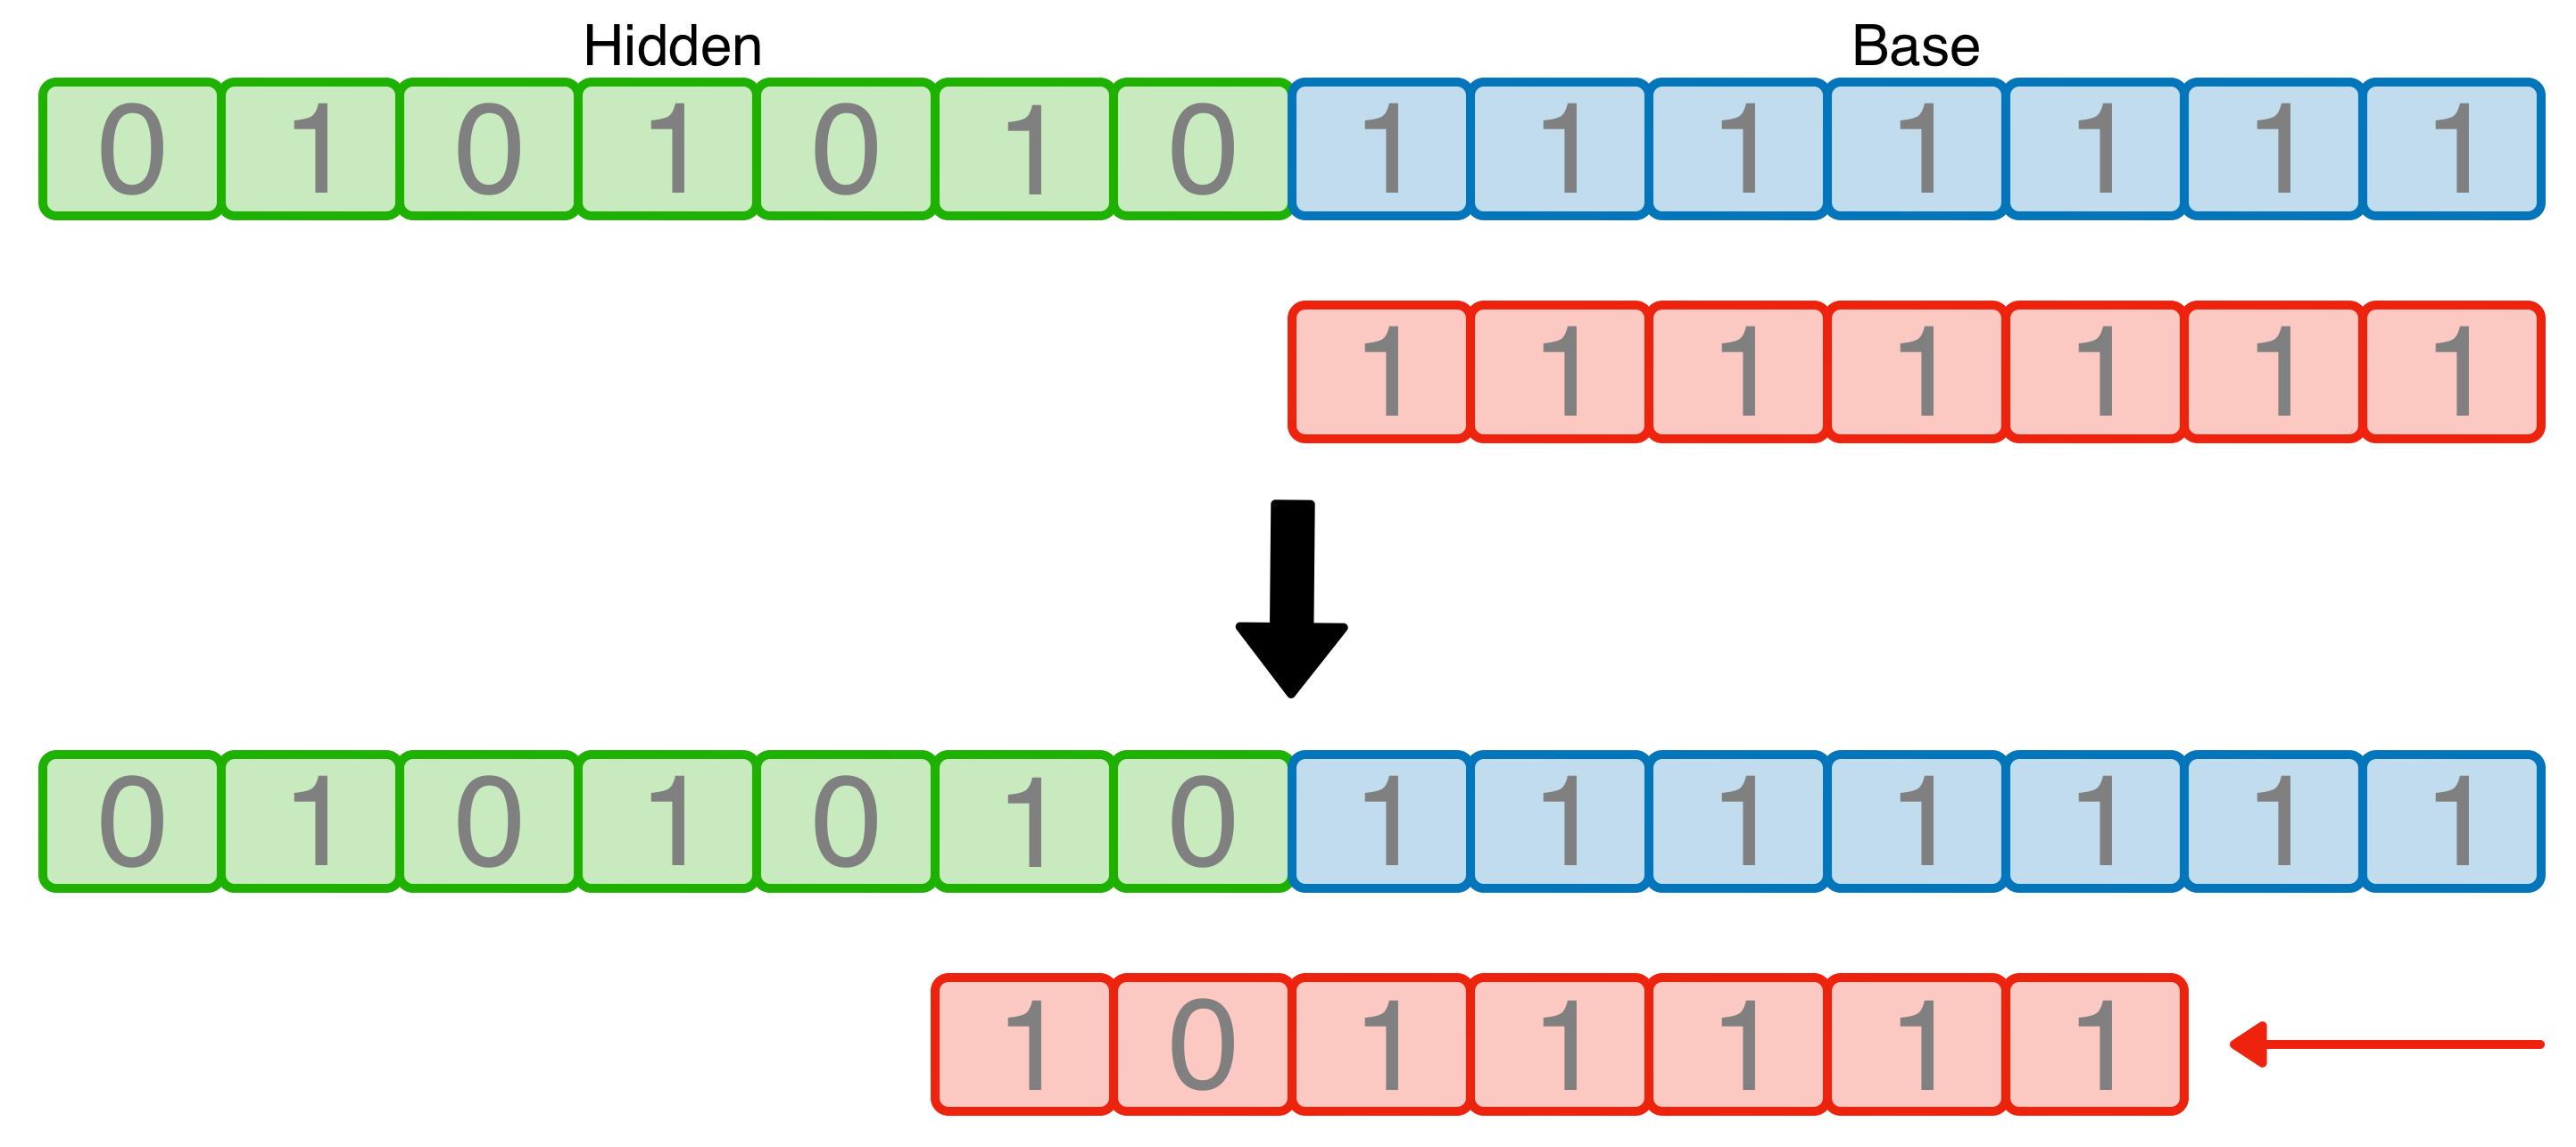
\includegraphics[width=0.75\textwidth]{gfx/ShiftRight.png}
    \begin{minipage}{0.49\textwidth}
        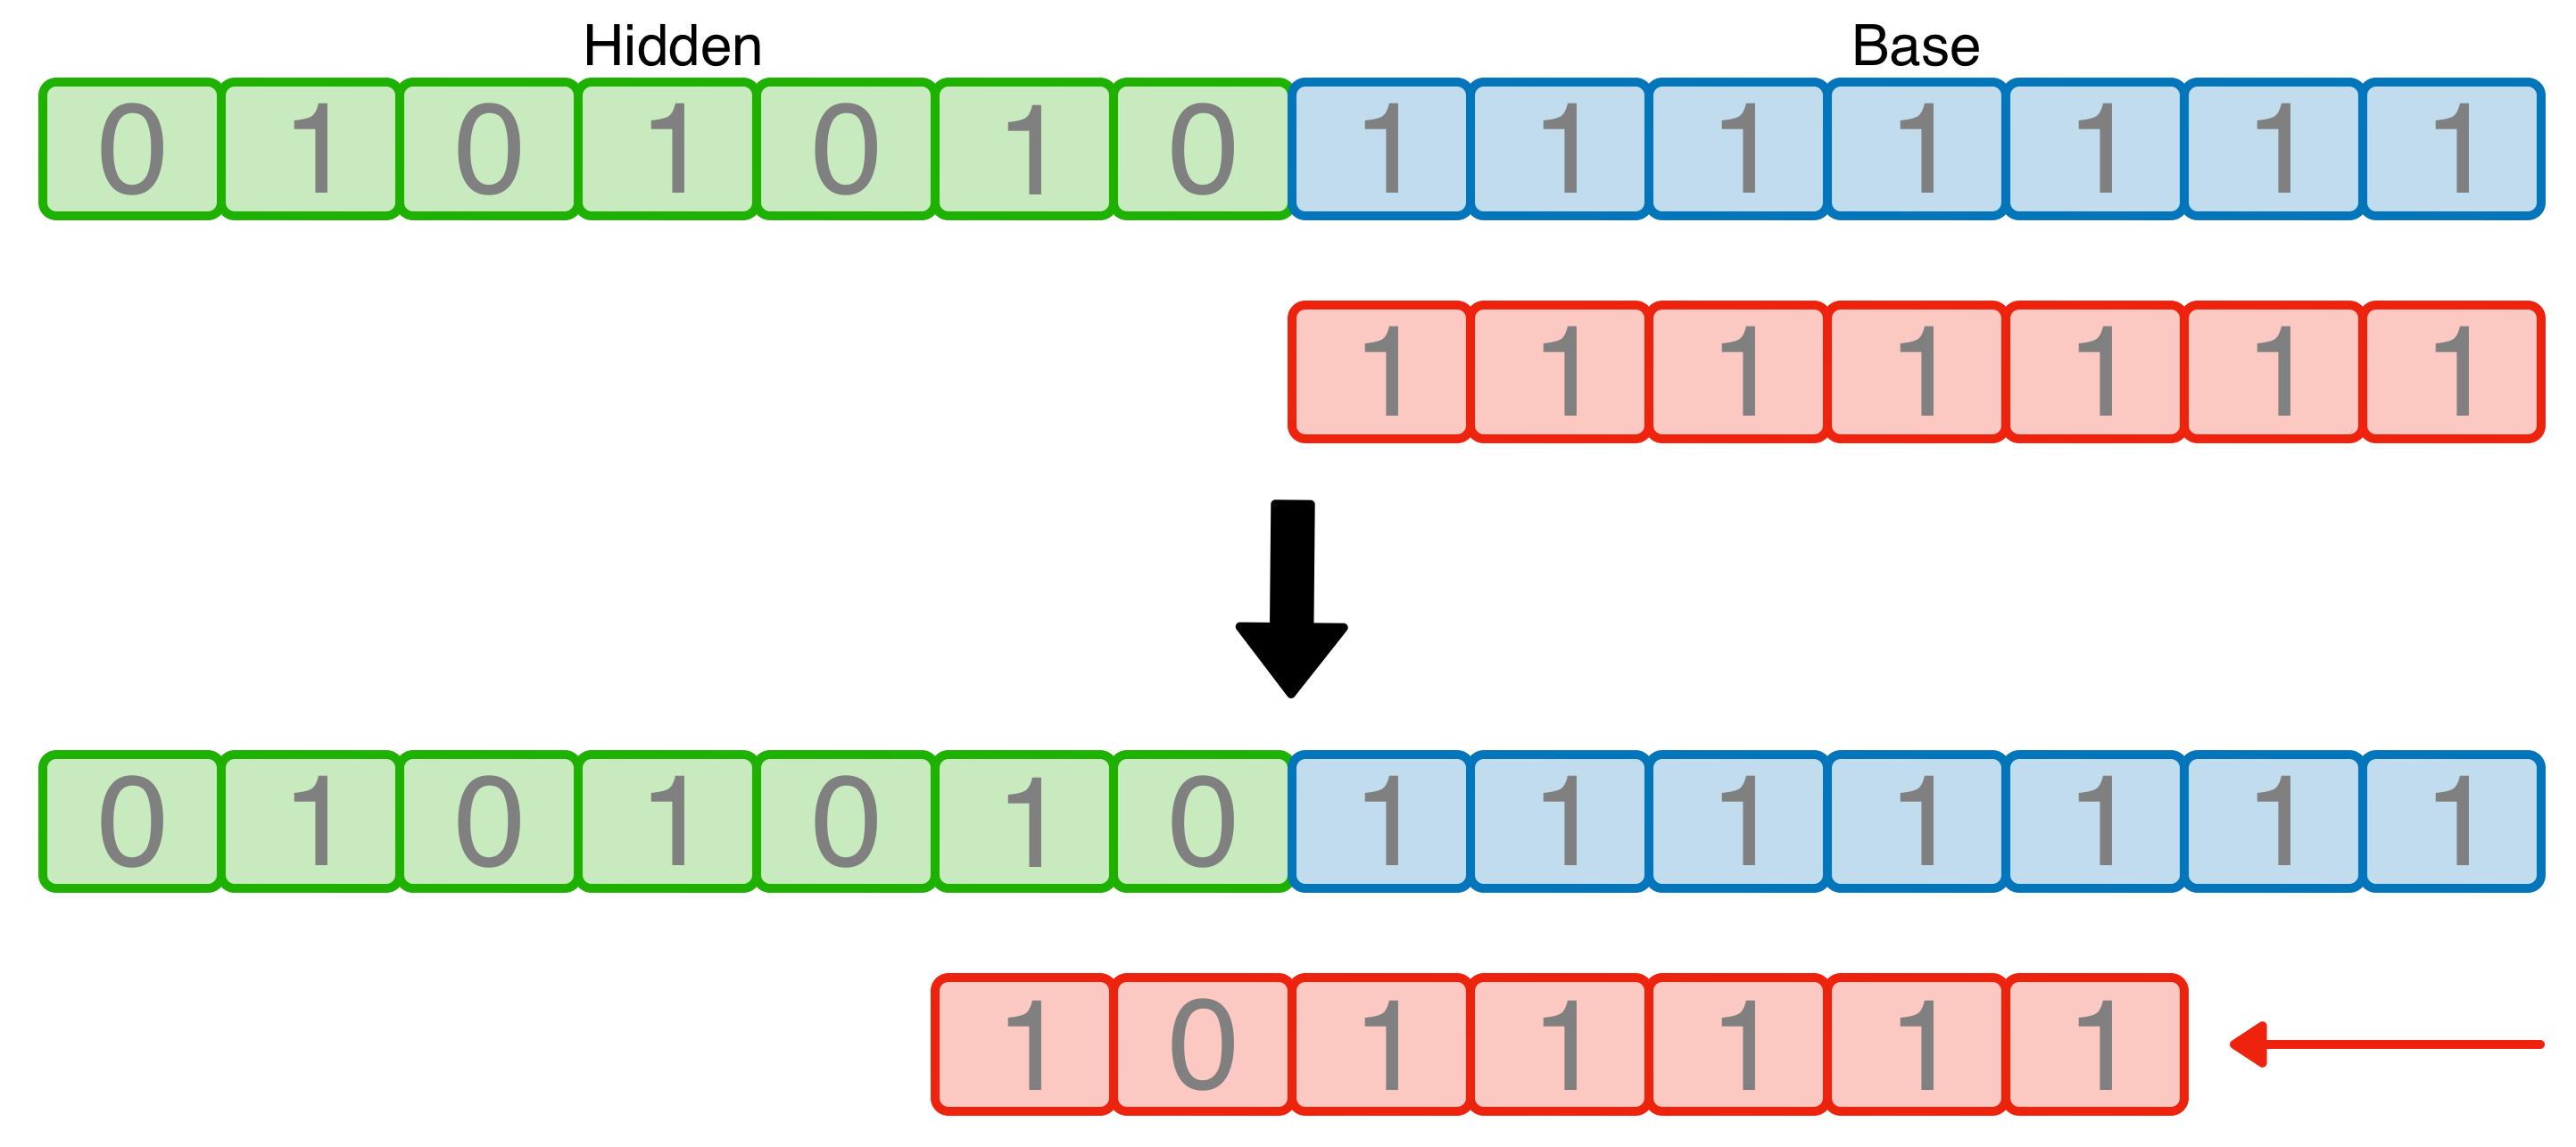
\includegraphics[width=\textwidth]{gfx/ShiftRight.png}
    \end{minipage}
    \hfill
    \begin{minipage}{0.49\textwidth}
        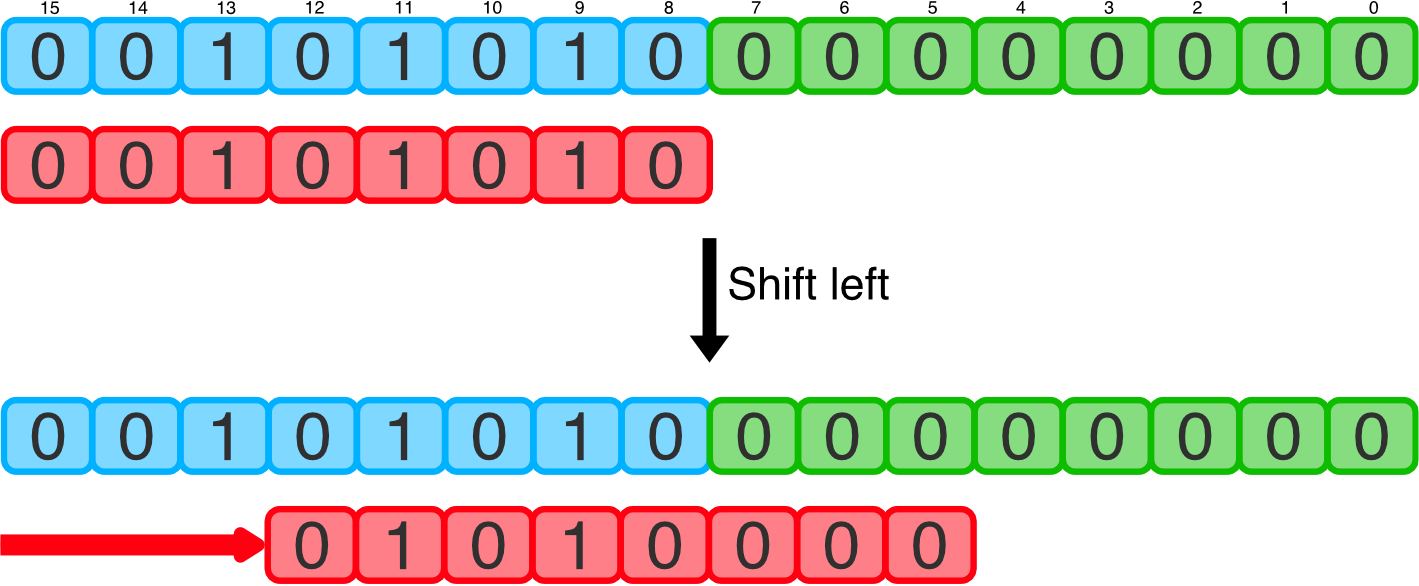
\includegraphics[width=\textwidth]{gfx/ShiftLeft.png}
    \end{minipage}
    \caption[A visual example of a right and a left shift.]{A visual example of a right shift by two, and a left shift by three. The green value represents the hidden value, the blue value represents the base value and the red value represents the value as visible.}
    \label{fig:shr}
\end{figure}

As we can see, this instruction is rather complex, and also transcends the conventional notion of shifts. Furthermore, the behavior of connecting signals and memory regions is not required at the IR level, but rather, it can be split in the frontend, resulting in operations acting on the two elements separately to obtain an equivalent behavior. For example, driving a connected signal is equivalent to driving the affected parts of the two signals independently, as illustrated in Figure~\ref{fig:drvconn}.

\begin{figure}[ht]
    \centering
    \begin{minipage}{0.49\textwidth}
        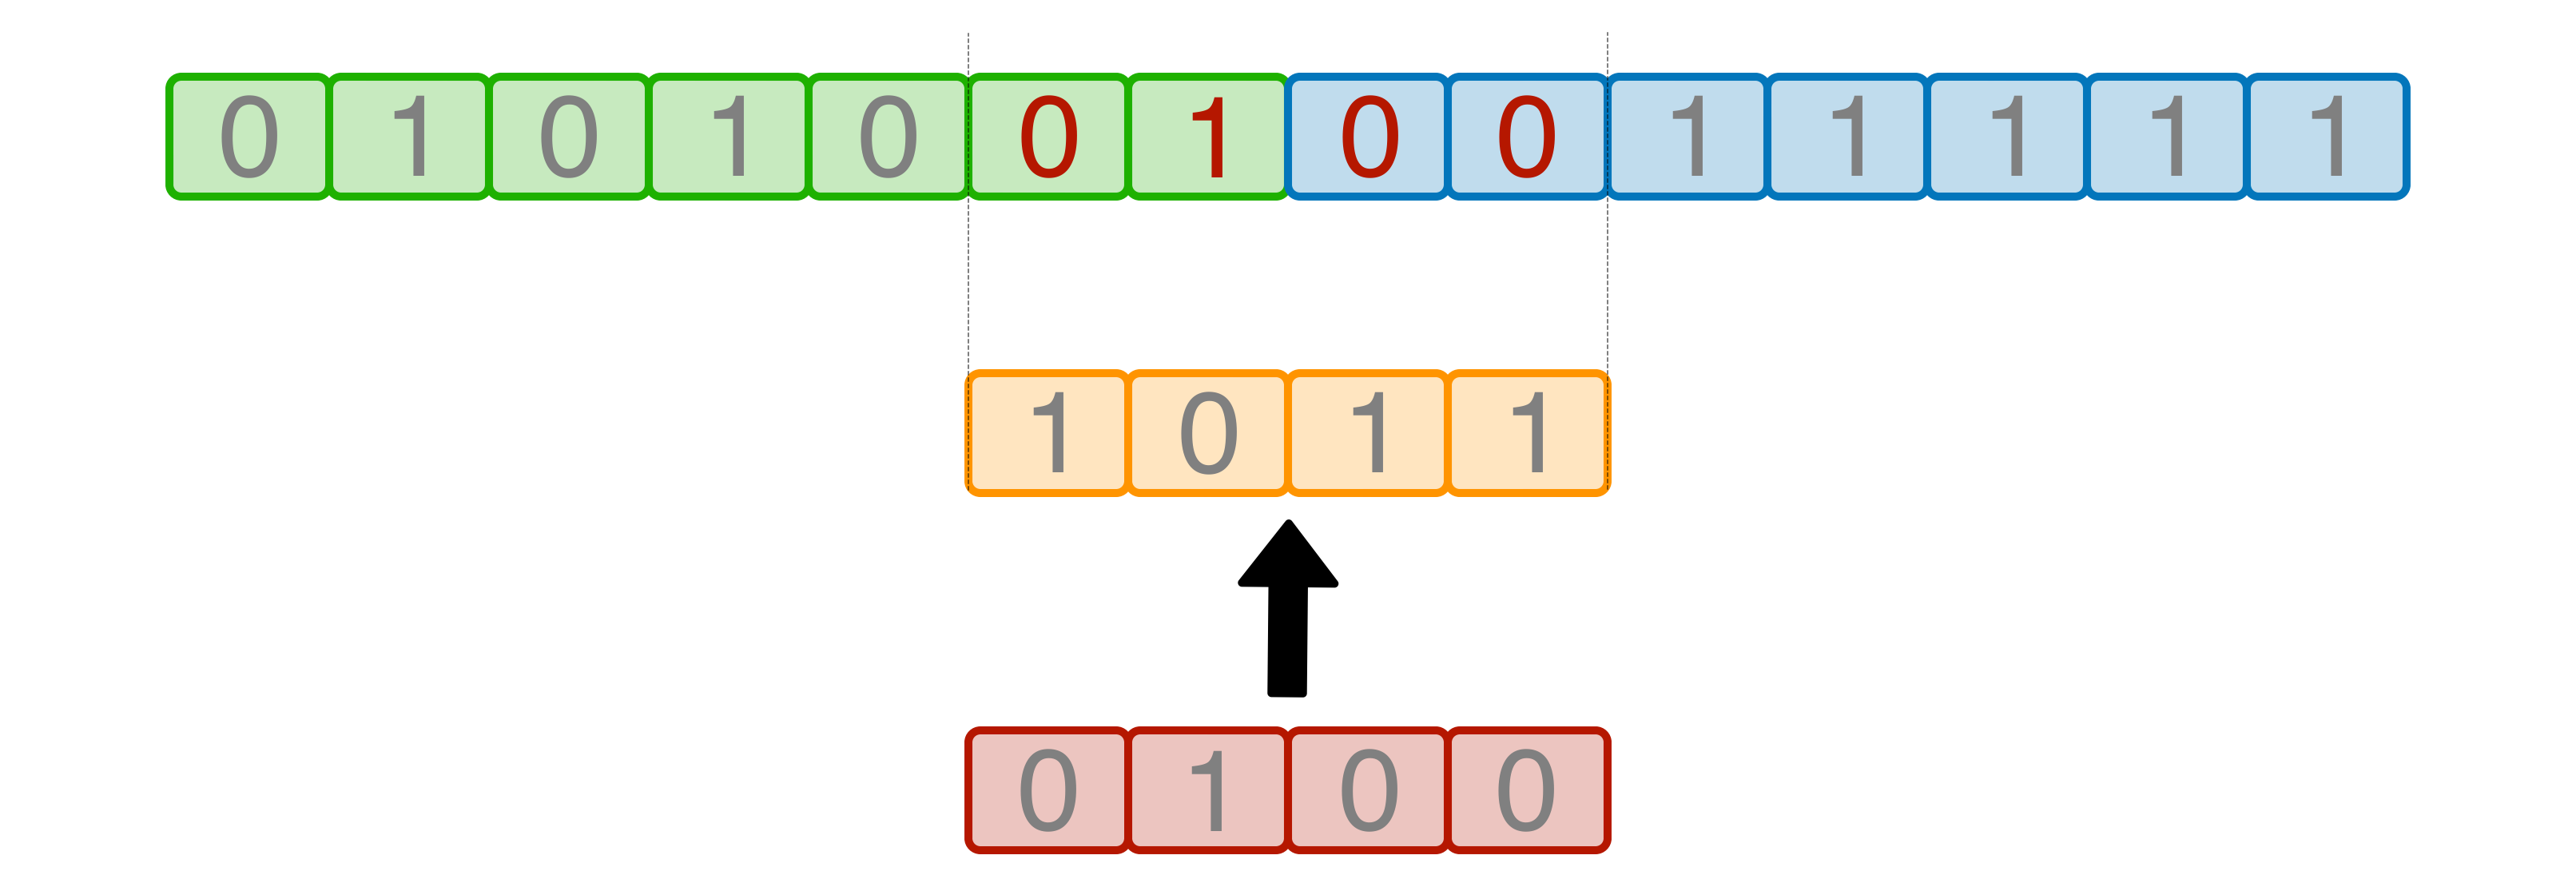
\includegraphics[width=\textwidth]{gfx/DrvConn.png}
    \end{minipage}
    \hfill
    \begin{minipage}{0.49\textwidth}
        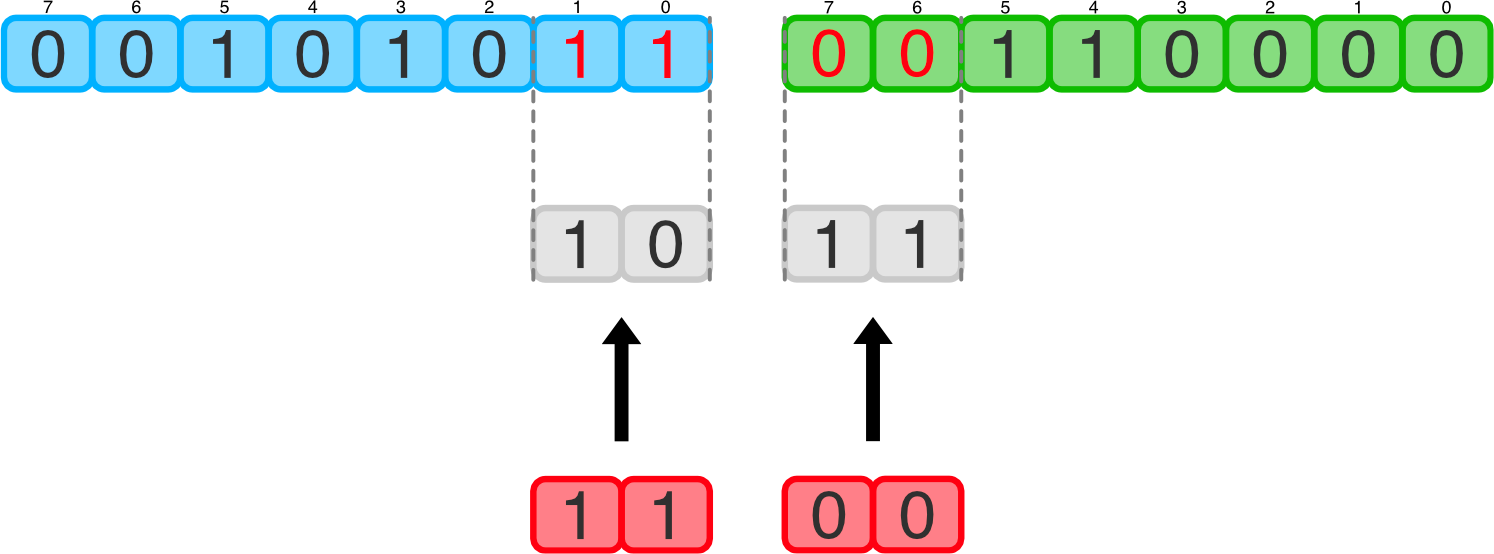
\includegraphics[width=\textwidth]{gfx/DrvSplit.png}
    \end{minipage}
    \caption[Driving a connected signal vs. driving the two origin signals independently.]{Illustration showing a drive to a connected signal (left) vs driving the two origin signals independently (right). The blue and green regions represent the two original signals, while the gray area represent their sub-signals. The red area and values represent the driven value.}
    \label{fig:drvconn}
\end{figure}

To simplify the semantics of those instructions, we decided not to support shifting pointers and signals anymore, and to switch to conventional semantics for signed and unsigned shifts. Here we will require to include the respective new operations in the LLHD dialect, to support the logic types, though this has not been implemented yet. We thus still have the original LLHD shifting operations in our dialect, \texttt{llhd.shr} and \texttt{llhd.shl}, to fully support \texttt{moore}-generated code until the new semantics are fully adopted.

The LLHD shift instruction also enables to dynamically drive only parts of a signal, when the starting index of the slice (or element) is not known at compile-time. We still need to represent such behavior, for which we introduced a dynamic variant for the \textit{extract slice} and \textit{extract field} operations, described below.

\paragraph{Extraction and insertion operations}
LLHD provides extraction (and insertion) operations to extract (resp. insert) elements or slices from integers, arrays, and structs. Furthermore, the extraction operations are also defined on pointers and signals of such types, acting similarly to LLVM's \texttt{getelementptr} instruction and the shift instruction. Namely, when used on signals and pointers, no value is probed (or loaded) from the respective signal (or memory location), instead, a new signal (or pointer) is created, pointing to the desired element (or start of a slice).

Extraction and insertion operations come in two variants: \textit{extract element} and \textit{extract slice}. In our MLIR representation, each of those variants is represented by a different operation. Both take an attribute representing the index of the desired element (or the start of the slice) in the target value. This means they can only work when the start index is known at compile-time. To work around this, \texttt{moore} commonly inserts first a shift, shifting the target value such that the desired index lands at the $0$-th position, and then extracts the desired value with index $0$.

Dynamic extraction, \ie, with a start index not statically known at compile-time, is very common in LLHD. LLHD's convoluted shift semantics are partially a consequence of this. To reduce the complexity of those operations, we introduced new dynamic extraction operations, aimed at eventually replacing those shift-and-extract patterns and the complex shift semantics in general. An example of the new extraction operations can be found in Listing~\ref{listing:extracts}, together with the static versions.

\mlirfile{An example of the extract operations.}{An example showing the syntax of the extract operations. The declarations of the various undefined operands are purposefully left out for readability.}{extracts}

\paragraph{Comparison operations}
MLIR provides a comparison operation for integers in the standard dialect, \texttt{cmpi}, which takes a predicate for the type of comparison to be executed (\eg, equality, or inequality). We use this operation for less-than and greater-than comparisons, but not for the equality instructions. LLHD defines the \textit{equal} and \textit{not-equal} operations on all types, including structured types, where an element-wise comparison is performed. The standard dialect's one, though, is only defined for integers. We thus introduced a \texttt{llhd.eq} operation and a \texttt{llhd.neq} operation to cover the case of structured types comparison.

% 03-simulation.tex

\chapter{Simulation}
\label{ch:sim}

Simulation is an important tool in hardware verification, together with formal verification \cite{YuanLu2001, Kumar1998}. It allows to ensure a design follows the expected behavior, as well as enabling comparison with the behavior of the manufactured circuit \cite{Ashenden1994}.

Furthermore, performing a correct simulation of our LLHD dialect allows us to assert that LLHD is in fact fully representable in MLIR.

We propose a first prototype of a simulator using LLHD's MLIR representation, called \texttt{llhd-sim} (same as the LLHD reference simulator). For this first prototype, we follow a similar approach to the \texttt{LLHD-Blaze} simulator \cite{Schuiki2020}, by leveraging Just-In-Time (\textit{JIT}) code generation, in combination with a MLIR conversion pass from LLHD dialect to the LLVM dialect, to enable the execution of the units, and a sequential event-driven algorithm to carry out a behavioral simulation of the design. With this first research prototype we can successfully simulate real-world designs such as a full \textit{Snitch} \cite{Zaruba2020} processor. A correctness and performance evaluation is provided in Chapter \ref{ch:eval}

%---------------------------------------------------------------------------------------------------

\section{Sequential Event-Driven Simulation}
Event-Driven Simulation algorithms \cite{Ashenden1994} view a physical design as a collection of physical processes. Physical processes then communicate with each other by reacting and generating time-stamped events, carrying the changes that happen to the physical signals during their execution. Each process can modify its local state, but only communicate with other processes through events. This means that process execution during a time-step is independent of all other processes executed during that time-step, where a \textit{time-step} represents a unique instant in simulation time. Correctness of the simulation can thus be guaranteed if a processes acts upon events in non-decreasing time-stamp order. We also note that the order in which events happening at the same time-step are processes is not defined, and is thus not relevant, since all the events in that step are independent of each other.

\begin{listing}[ht]
    \caption{Sequential event-driven simulation algorithm.}
    \label{listing:seqEDS}
    \begin{minted}[
        frame=lines,
        framesep=2mm,
        baselinestretch=1.0,
        bgcolor=lightgray!10,
        fontsize=\footnotesize, linenos
        ]{c}
initialize all logical processes
while event-queue EQ not empty do
    set global simulation time to timestamp of first event in EQ
    pop the first element in EQ and resume destination process
    enqueue any new events scheduled by the process
    \end{minted}
\end{listing}

In a sequential implementation, as shown in Listing \ref{listing:seqEDS}, events are typically collected an ordered queue of events (the \textit{event queue}). Here, events to be processed at later time-steps are stored in ascending time-stamp order. The body of the loop represents a simulation cycle. In each cycle, one event is processed. Since the event-queue is ordered by the time-stamps, this also guarantees the correctness of the algorithm.

%---------------------------------------------------------------------------------------------------

\section{LLHD simulation}
In LLHD, each unit (both entities and processes) represents one physical process. Each process can be sensible to a (sub-) set of all the signals present in the design.

In the case of an entity, its body is executed in its entirety each time one of the entity's owned signals (signals defined in that entity's body) or an input (or output) signal changes.

Processes on the other side can suspend their execution before the end of the body is reached. Furthermore, they can include control-flow loops and potentially run indefinitely. Generally speaking, the only way of completely stopping a process' execution is for it to reach a halt operation, which prevents the process from ever waking up again. A process execution thus usually resumes at the block targeted by the last wait operation that suspended a previous execution, whenever an observed signal changes, or we reach the time of a scheduled wake-up. The only exceptions to this is the first execution, where the process starts at the entry block.

\begin{listing}[ht]
    \caption{Revisited sequential event-driven simulation algorithm used to simulate LLHD.}
    \label{listing:seqLLHD}
    \begin{minted}[
    frame=lines,
    framesep=2mm,
    baselinestretch=1.0,
    bgcolor=lightgray!10,
    fontsize=\footnotesize, linenos
  ]{c}
initialize all logical processes
while event-queue EQ not empty do
    set global simulation time to timestamp of first event in EQ
    pop the first element in EQ
    apply the signal changes scheduled by the event
    wake up all sensitive units
    enqueue any new events scheduled by the units
\end{minted}
\end{listing}

Listing \ref{listing:seqLLHD} revisits the sequential algorithm from Listing \ref{listing:seqEDS} to fit it to our needs. For each cycle, we build a wake-up queue, which lists all the units that require to be executed in that cycle. After updating the global simulation time, the signal changes scheduled in the event are first processed, which also fill \textit{wake-up queue}. All units in the wake-up queue are then executed, and all new events are finally queued in the event-queue. We also note that we generate only one event for each unique instant, and this contains all the signal changes occurring in that instant, instead of having one event for each signal change. This allows us to both reduce the event-queue size and number of unit executions, while still guaranteeing simulation correctness, since all those changes are independent, as previously described.

Following this revisited algorithm, we build a simulator using the structures described in Section \ref{sec:structs} to maintain the simulation state, and JIT compilation to execute LLHD units, as described in Section \ref{sec:execution}.

%-------------------------------------------------------------------------------

\subsection{Simulator Structures}
\label{sec:structs}
To be able to perform a simulation, we first need a means to keep track of the global simulation state and track all the relevant information necessary to proceed through the simulation. To do this we use a series of data structures as basic building blocks of the global simulation state. In this section, we discuss their shape and use.

%---

\subsubsection{Time and Signals}
At the base of the simulator, we have a representation of time and signals.

A time unit can be simply represented by three values, representing real-time, delta step and epsilon step.

For signals on the other hand, we require keeping track of some more information. Each signal can be uniquely identified through its name and owner instance. This enables us to identify signals in cases where their location in the global signal table is unknown. The name in particular is also required to identify the various signals in the generated simulation trace.

Each signal also owns a memory region in the heap, where its value is stored. A pointer to this region is always stored for each signal, together with the size the signal type occupies in memory. We require keeping track of this information for making the signals available to units during unit execution (see Section \ref{sec:execution}), signal changes processing, and trace generation (see Section \ref{sec:trace}).

A signal update always results in a subset of all instances being triggered. To be able to retrieve all of them with ease, without the need of searching each instance for each signal change, we store a list of all sensitive instances here as well. Figure \ref{fig:sig} shows the final shape of the signal structure.

\begin{figure}[ht]
    \centering
    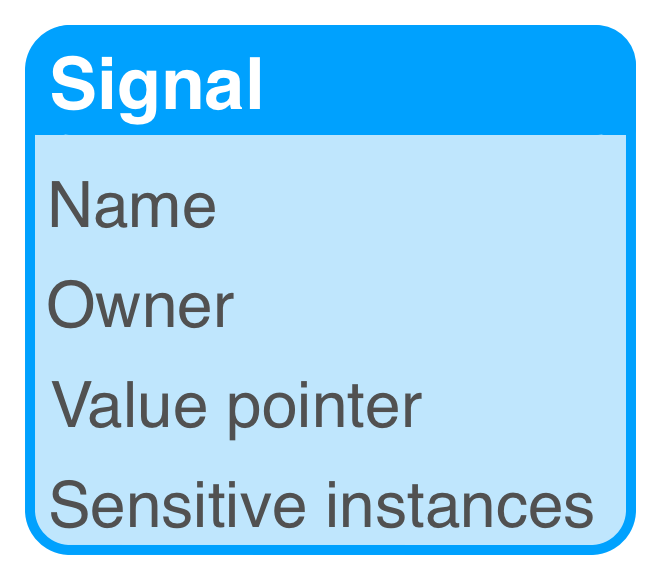
\includegraphics[width=0.4\textwidth]{gfx/Signal.png}
    \caption{<PH> The data structure used to represent a signal in the global simulation state}
    \label{fig:sig}
\end{figure}

%---

\subsubsection{Instances}
Each instance represents a “copy“ of a unit, and different instances of the same unit can coexist, with different input and output signals connected to them.

We thus keep track of various information about instances, starting from their name, base unit and placement in the design hierarchy. The latter is achieved by keeping track of the parent instance, thus building a linked tree of the hierarchy, with the root instance on top. Note though, that this was initially used to generate the hierarchical paths during trace generation, but to avoid regenerating the path each time a signal change is dumped, we store the full hierarchical path as a string in the representation of an instance. It is not yet clear if we will require knowledge of the hierarchy of the design at that granularity, thus we left this in the current implementation.

As mentioned, each instance has a set of signals it is sensible to. Those can be either owned be the instance itself, in case of an entity, or be connected through one of the input or output ports. For each of those signals, we store an entry in a local signal table, which contains the pointer to the signal value, a value representing it's offset in the first byte, and index in the global signal table and instance signal table, in order to make them easily available to units during their execution. The use of this information will be explained in more detail later. Also note, that this does not correspond to the signal representation described above.

Entities and processes also require different local states to be able to correctly execute. In the former case, the only additional local state required during execution is for the reg operation trigger values contained in the entity: to be able to detect a rising or falling edge of the trigger, the current SSA operand's value is not enough, but we always need information about its value in the previous execution.

For processes on the other hand, more information is required: since processes can suspend their execution at any terminator in their body (through a wait operation), we need to keep track of where we need to resume execution. This can be achieved by indexing all the possible resume points, and storing the current index into the state.

Another problem arises with value persistence, namely, since the body is no more fully executed, the process would resume and try access undefined values. We avoid that by storing all required values in the process' local state, a detailed description of how this is achieved can be found in Section \ref{sec:execution}. Finally, process suspension can also restrict the sensitivity of the instance to given subset of the argument signals. This behavior can be represented by storing a flag for each signal in the instance's sensitivity list, indicating if a signal is enabled.

%---

\subsubsection{Events and Event Queue}
An event (or \textit{time-slot}) in our simulator, as we defined at the beginning of this section, contains a list of signal changes rather than only one signal update. If multiple drives to the same signal are scheduled in the same time-step then only the last one in order of execution will be visible in the trace. We recall that this does not affect correctness, as the order updates at the same instant is not defined. Within a slot, we represent this by mapping signals to a list of signal updates, for each signal that has changes scheduled in that slot. Since processes can also have a timed suspension, we also keep a list of processes that are scheduled to wake up in that slot.

With a slot as the building block, we can construct the event-queue as a priority queue ordered by the slot's time. Each slot becomes an entry in the queue, and is placed in the correct order, such that popping the queue is always guaranteed to take the earliest possible event.

%---

\subsubsection{Global Simulation State}
Finally, we can build the global simulation state. Here we store the current simulation time, as well as a global list of signals, the list of instances in the design, and finally the event queue.

To initialize the signal and instance structures, we analyze the input design during a first state initialization step, gathering all the relevant information about the design. The initialization of the signal values and instances local states though, happens in a different step, and is handled by the conversion pass described in the next section.

%-------------------------------------------------------------------------------

\subsection{Unit Execution}
\label{sec:execution}
To be able to perform a simulation, we need a means to emulate the behavior of a circuit. We observe that LLHD shares many similarities with the LLVM IR, and that a mapping from LLHD to LLVM IR is therefore mostly trivial. We can thus define a MLIR conversion pass from our LLHD dialect to the LLVM dialect, and then we can get the various units of a design as callable function pointer, by feeding the converted module to a \textit{Just In Time} (\textit{JIT}) compiler (MLIR's \texttt{ExecutionEngine} in our case). As mentioned in Section \ref{section:mlir}, a conversion pass is mainly composed of a set of patterns that match a given operation, and define a legal conversion for it. Where we require direct interaction with the simulator's state, \eg for spawning events, we make use of a small runtime library, containing functions that can be called by the converted code.

In this section we will describe how we can fully map LLHD to LLVM dialect. We leave out a full description of some of the most trivial conversion, such as most of the bitwise operation, that can be mapped one-to-one to the LLVM dialect in our current implementation.
% Following, we will describe some of the most involving conversions, while the remaining operations have a trivial mapping to LLVM dialect.

%---

\subsubsection{Mapping LLHD Types to LLVM Types}
\label{sec:typeconv}
For integers and tuples we use standard types. The conversions for those types is thus already defined by the standard to LLVM dialect conversion. There, both integers and tuples get converted to equivalent LLVM dialect types.

To map a signal to LLVM dialect, we require keeping track of various important information. First and foremost we need a pointer to the memory region where we store the current signal's value. We also require keeping track of a potential bit-offset into the first byte. To fully represent a sub-signal we would thus need bit-granularity pointers, since integer sub-signals can start at any element (or bit) of the original signal, while memory is generally byte-addressed, so we can represent sub-signals as a tuple containing the pointer to the byte where the sub-signal starts, together with an offset into the first byte, representing where the sub-signal actually starts at a bit-granularity.

Further information we keep track of for signals are the index of the signal in the global signal table, and the index of the signal in the local signal table. The former index is useful to retrieve the signal in occasions such as a drive, without needing to rely on arbitrary assumptions at compile time (such as the order the operations are processed during the conversion). The latter is necessary to determine which signals to enable or disable when a process suspends its execution through a wait instruction.

Signal information can not be hard-coded into the entity mapping, as it's generally not unique, but rather changes depending on which instance of the unit we want to run. We thus need a dynamic way to make each instance's specific signal table available to the entity lowering. For those reasons, we map a signal to a pointer into a struct containing all relevant information described above, and a unit's signal table (containing both the argument signals and the newly defined signals) is then mapped an array of signal structures. This way, each signal becomes a pointer to one of the elements of the argument signal table, and the signal's information can be loaded on-demand where it is needed.

% Furthermore, a signal initialization should only happen once, and not be performed each time the unit is run. We thus defer the signal allocation role to the inst operation, as we will describe later, and leave to a sig operation the only role of retrieving the correct signal. As we will describe in more detail in the next section, we expose signal information through function argument, common to all units (entities and processes alike).

% This information is vital in a correct execution in our current implementation. The value pointer is self-explanatory. The byte offset represents the offset of the signal in the first byte of the pointer. x86 systems use a byte-addressed memory model, meaning that we cannot obtain bit-precision granularity with pointers. This is no problem for normal signals, but becomes a problem in the case of sub-signals, generated from extract and shift operations, where a sub-byte offset into a byte is can occur. For example, shifting a signal right by one bit would result require a pointer with one bit offset into the original signal. This is not representable with just pointer, so we represent it as the same pointer, but with a byte-offset of $1$.

% We require to consider those offsets when probing an integer signal. Thus, the \texttt{llhd.prb} operation can not just be converted to a \texttt{llvm.load} operation, but rather, it requires loading more than the signal's carried value width (we always load one extra byte), right-shift the value by the byte offset, and finally truncate the value to the intended width. We don't require those distinctions when working with structured types (arrays and tuples), as they're already byte-aligned.

% To drive a signal, we use one of function from the runtime library mentioned above. Since the signal update doesn't happen immediately, but after a delay, we cannot just store the new value to the signal pointer. So we store it to a newly stack-allocated pointer first, and pass it, together with its width, to the runtime function. This runtime function, \texttt{drive\_signal}, copies this value to an \texttt{llvm::APInt}, a \texttt{C++} class to represent arbitrary-precision integers, and spawns a new event (or adds the change to an existing event if it already exists).

As mentioned in Chapter \ref{ch:ir}, LLVM arrays offer the flexibility we need for LLHD arrays, and we implemented our own type because we would be limited to LLVM types, and to generally have an easier time working with that type. Though when mapping LLHD to LLVM dialect, since we're mapping all LLHD types to LLVM types, we can now represent LLHD arrays as a one-to-one conversion to LLVM arrays of equivalent types.

We currently map pointers one-to-one to LLVM dialect pointers. This means though, we currently have no way to represent an extract on an integer pointer, whenever the new pointer should be starting within a byte. In the future, we will need to maintain byte-offset information, similar to signals, for example by converting LLHD pointers to LLVM structs containing a pointer and a bit-offset.

%---

\subsubsection{Unit Conversion}
To represent entities and processes, we use LLVM functions with a static and predetermined signature, which replaces the original unit signature. The new signature contains a pointer to the global state and the signal table array described above. A final argument represents the unit's local state. Here entities and processes will receive a pointer to the respective state type which is determined for each unit. More precisely, for entities, the local state will contain the value each reg operation's trigger assumed in its last execution. Processes on the other side require to maintain a local state for all the values that require to be persisted across process suspension, as well as a resume index, and a flag-array containing one entry for each argument signal, indicating if the process is currently sensitive to a given signal.

Since the original signature of the unit is stripped away, the signal operands are now undefined, and those signals reside instead as an element of the new signal table argument. For each of the signals in the signal table, we thus need to replace their uses with a pointer to the correct element in the signal table. For signals that were originally part of the unit's signature, a \texttt{llvm.getelementptr} operation into the signal table argument is inserted at the beginning of the unit's body, while \texttt{llhd.sig} operations can be converted to \texttt{getelementptr} operations at their original location.

To lower entity bodies, we observe that although they are defined to be following the data-flow paradigm, rather than control-flow (meaning the order the instructions appear in doesn't matter, and they should be executed following the \textit{Data-Flow Graph}), LLHD still adheres to the SSA dominance condition (all SSA operands are declared before their use). This means that when no control-flow operations are present, such as branches, the Data-Flow Graph matches the \textit{Control-Flow Graph} (CFG). Also, at the time of implementing our dialect, there was no way to work around the dominance condition in MLIR, and \texttt{llhd.entity} bodies consequently have to adhere to it to be legal, further enforcing our observation. As a consequence, entity bodies don't require to be re-ordered to follow the DFG, and we can in-line them as they are into the converted entity function.

Process bodies require some further processing, namely, we need to generate logic for process suspension and resumption. Although process suspension is per se dictated by the \texttt{llhd.wait} operation, and this step seems more adequate to be part of the wait operation's lowering at first glance, we argue that this operation's effect spans across the whole process. Furthermore, during the execution the process lowering pattern, we have a broader view of the whole process easily available. In fact, a pattern of a MLIR pass usually receives only information about the operation it is matching, and tracking back information about other operations is not always trivial and sometimes requires arbitrary assumptions (\eg that another operation has not been converted).

Enabling process suspension and resumption execution requires two main considerations:
\begin{enumerate}
    \item We require knowing where in the process' body execution has to be resumed. We know that suspension can only happen at a block terminator, while resumption can only be at the beginning of a block. We can thus maintain an index, telling us what is the block we need to resume execution to, and insert a series of new blocks at the beginning of the body. Each of these blocks, we call them \textit{comparison blocks}, compare the index with one of the possible resume indexes, and then conditionally branches to the resume block, in case the index matches, or to the next block otherwise. This mimics the behavior of the LLVM IR \textit{switch} operation, which is unfortunately missing in the MLIR dialect.
    \item We require to restore all the values that the process uses after resumption to the values they had before suspension. In a first naïve and very conservative implementation, we store each value that “escapes“ its defining block in the process' state, and load them from the local state whenever used outside their defining block. Since suspension can only happen at the end of a block, and resumption can only happen at the beginning of a block, this ensures we always have all the values we need available, at the cost of persisting additional values, which would otherwise not require to be persisted. In the future, approaches such as Temporal Region Analysis could be used to determine which values actually require to be persisted and avoid redundant memory accesses.
\end{enumerate}

In Figure \ref{fig:proclow} we illustrate a simple process conversion.

\begin{figure}[ht]
    \centering
    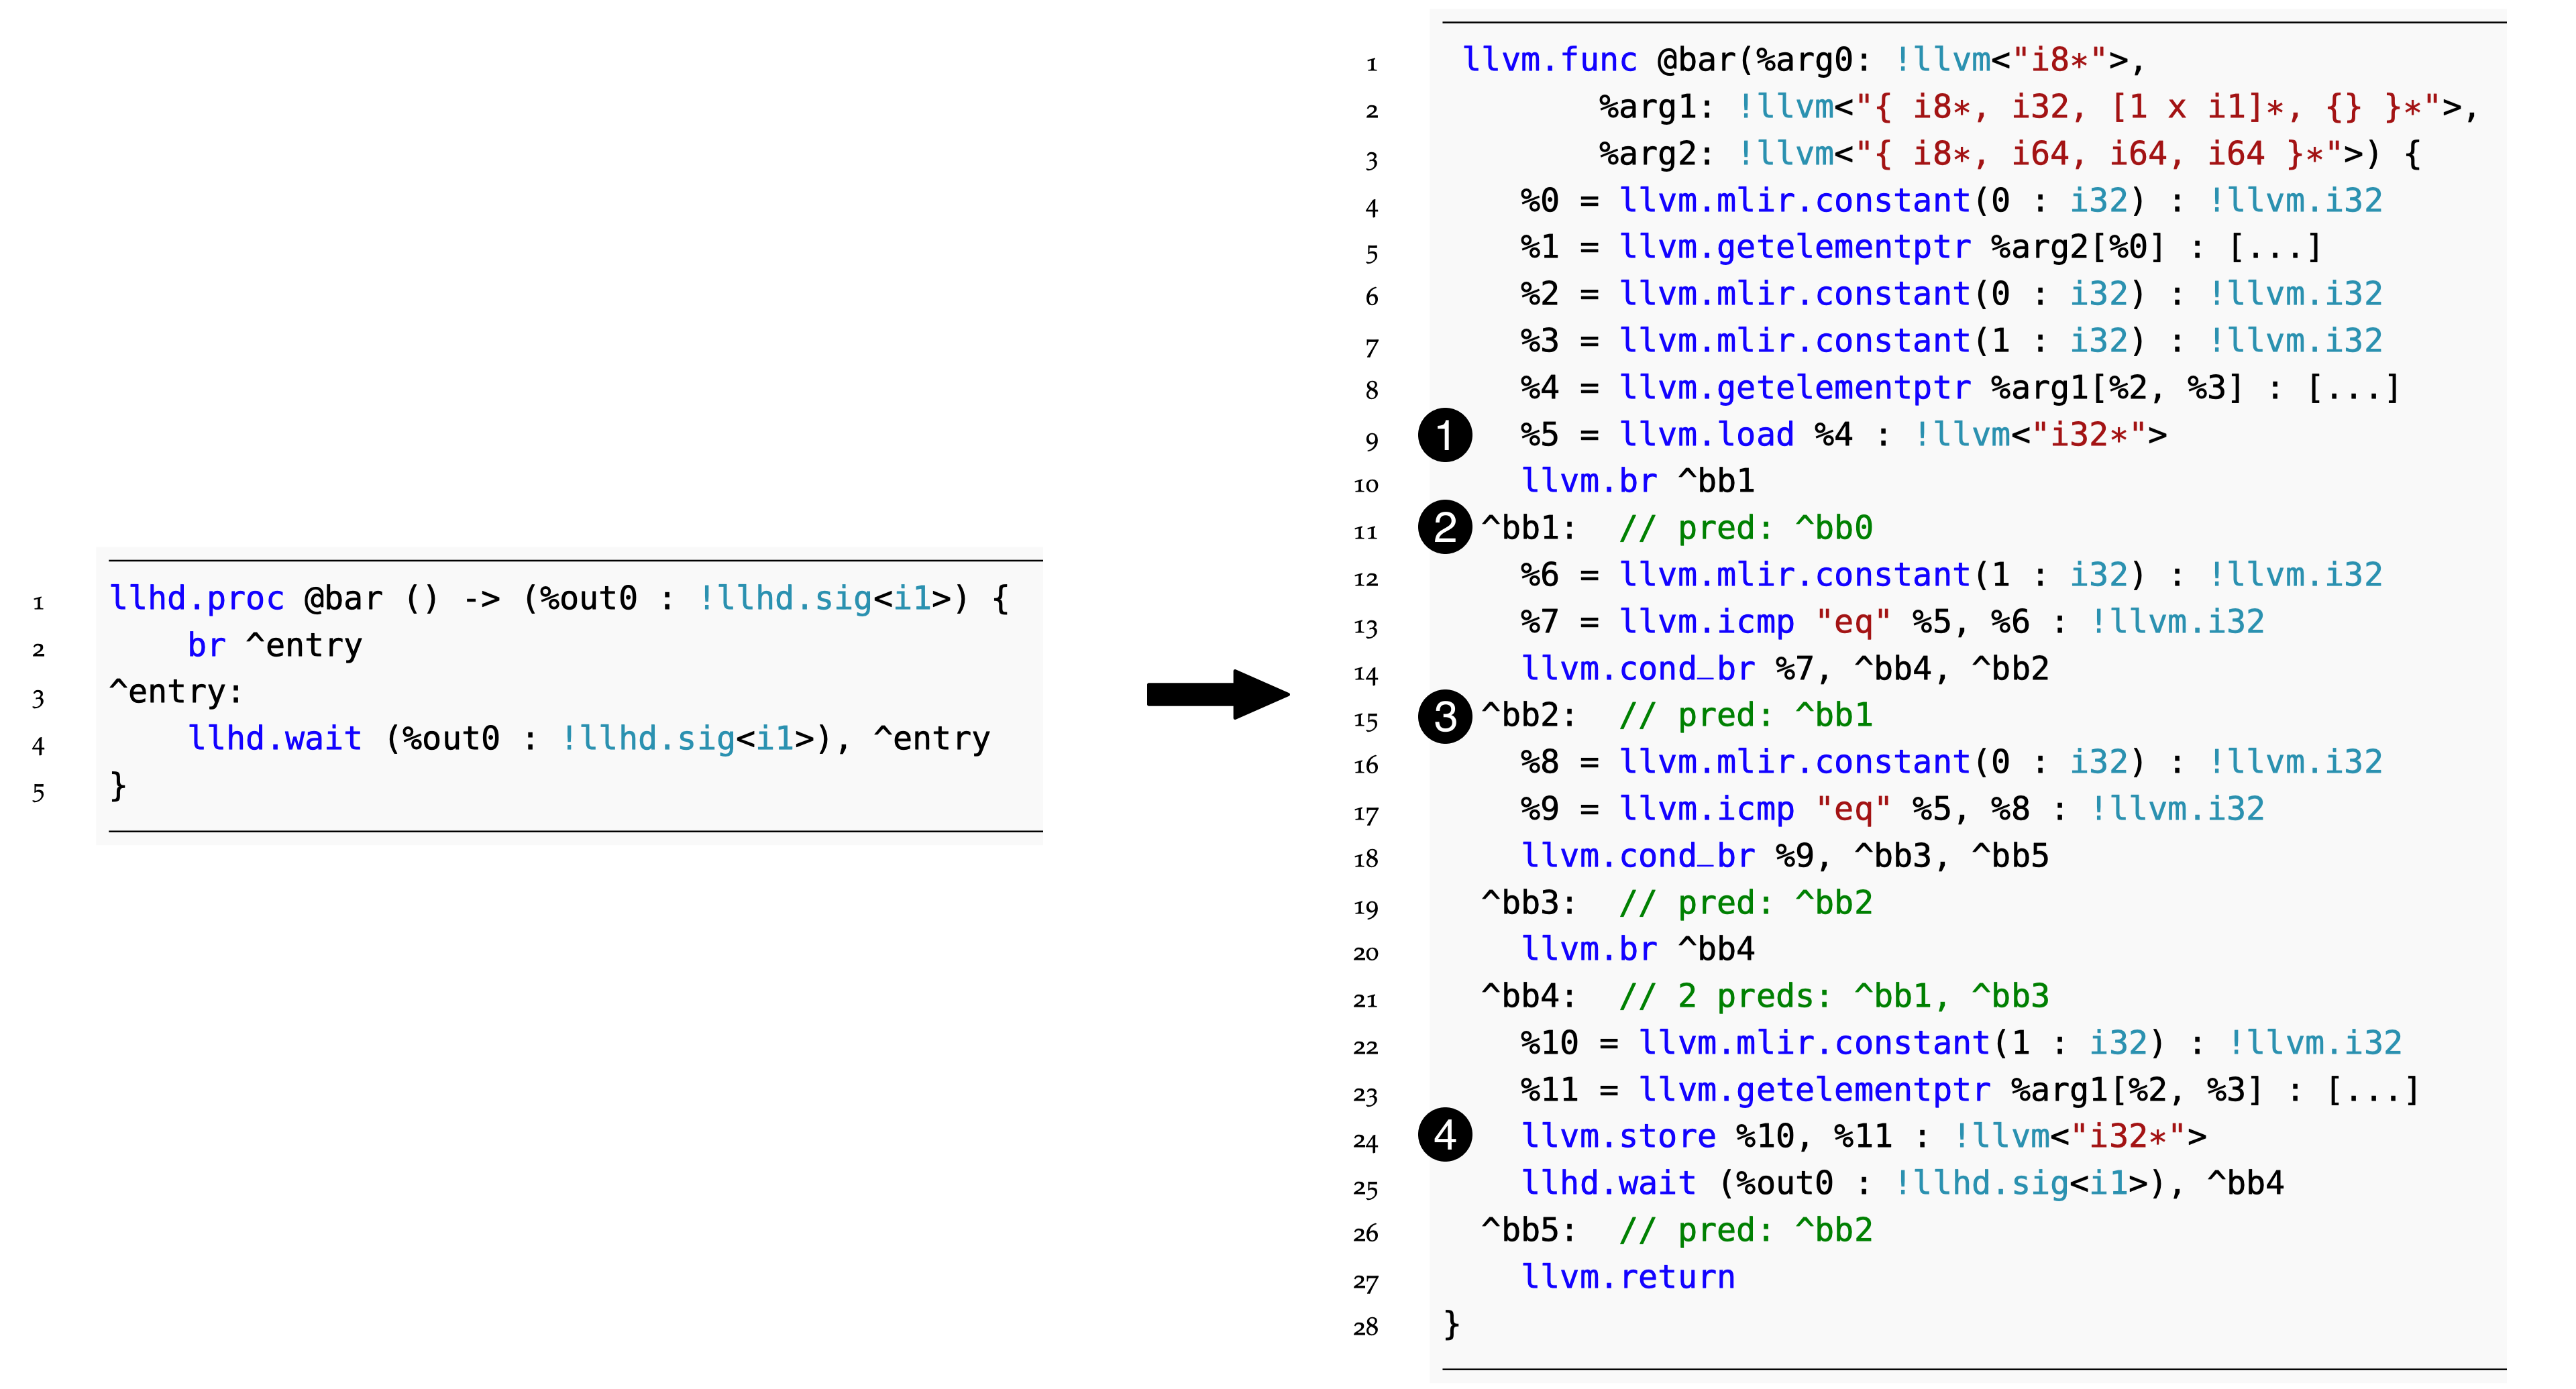
\includegraphics[width=1.1\textwidth]{gfx/ProcConv.png}
    \caption[A simple example of process suspension logic generation.]{A simple example of process suspension logic generation. First, the resume index is loaded from the state (1). We then compare it against the first possible resume index (2). In case the index matches this value, the execution is resumed at \texttt{bb4}, else the index is compared against the second possible index (\ie $0$) in the second comparison block (3). If that is the case, we are executing the process for the first time, and we jump to \texttt{bb3}. Otherwise, we are in an illegal state and interrupt execution. The resume index is finally updated before the wait operation (4).}
    \label{fig:proclow}
\end{figure}

% To enable execution resumption, we first require to store all relevant values before the process is suspended, and load them back after the process is resumed. As a naïve first approach, we use as criteria to find the values that need persistence, whether they escape their defining block, meaning that we will store in the process state all those values that are used at least once outside the block they are defined in, and then replace all uses outside the defining block with the value loaded from the state. This is enough to ensure all required values are made available after process is resumed, since we cannot suspend execution in the middle of a block, but it introduces some level of redundancy in what values we persist in the state, that we accepted for the sake of simplicity in this first implementation. Figure \ref{fig:proclow} shows a simple example of this intermediate conversion.
% Finally, we need a means to resume execution at a given block. This can be done by introducing a series of new basic blocks, that we call \textit{comparison blocks}, to compare the current resume index with all possible resume indexes, and conditionally branch to the correct block. In each of those blocks, the conditional branch terminator jumps to the next block on a false, except of the last comparison block, where the target for a false match is an additional dummy block, that interrupts execution, representing an illegal state.

Finally, since we're using the MLIR standard functions, we can directly use the standard dialect's conversion patterns to convert them to LLVM dialect.

%---

\subsubsection{Instantiation Conversion}
As mentioned above, for each \texttt{llhd.inst} operation, a “copy“ of the unit is instantiated. This means that we require to also initialize a copy of each of the signals declared by the unit, as well as allocating memory for a new copy of the unit's local state. We accomplish this by generating an initialization function through the instantiation conversion.

In more detail, the \texttt{llhd.inst} conversion pattern walks over the target unit once,  generating \texttt{malloc} calls in the initialization function for each of the declared signals. We also note that we currently allocate double the required space for each of the signals. This is to cover the case of shifting signals, where probing a signal could result in accesses outside of the allocated memory region. Once support for the old LLHD shift instruction is removed, as discussed in Chapter \ref{ch:ir}, we should also be able to reduce the space we allocate for signals.

Finally, we also generate \texttt{malloc} calls for the unit's local state and store all the generated pointers in the global state through some runtime function calls.

Important to note is that this approach requires us to guarantee that no other operation has been converted during the initialization function generation. Particularly, in the case of units we lose information about if they represent an entity or a process. Similarly, for signals we lose information about the carried type after the conversion. We thus need to convert the instantiation operations before anything else, by running a first partial conversion, followed by the full conversion. It is not yet clear if it would be worth to have a separate pass for this step, as it would have no use outside this pipeline.

% We also note that this requires all LLHD operation not to be converted, or we would lose some information about the structure of the unit's body, for example a process will not be distinguishable from an entity once converted, since both become \texttt{llvm.func} operations. To ensure this, we lower all the instantiation operations separately in a partial conversion call, before going on with the conversion of the remaining operations.

% \begin{listing}[ht]
%     \caption{proc intermediate example}
%     \inputminted[
%         frame=lines,
%         framesep=2mm,
%         baselinestretch=1.0,
%         bgcolor=lightgray!10,
%         fontsize=\footnotesize, linenos
%     ]{mlir.py:MLIRLexer -x}{examples/proc_lowinit.mlir}
%     \inputminted[
%         frame=lines,
%         framesep=2mm,
%         baselinestretch=1.0,
%         bgcolor=lightgray!10,
%         fontsize=\footnotesize, linenos
%     ]{mlir.py:MLIRLexer -x}{examples/proc_intermediate.mlir}
% \end{listing}

%---

\subsubsection{Extraction conversion}
\label{sec:extrs}
The extraction operations are between the most complex LLHD operations. They can operate on almost any LLHD type, and the semantics of the LLVM dialect mapping varies slightly for almost each of those types. For integers and structured types, the conversion is straight forward: for integers it is enough to shift the value and truncate it to the desired bit-width. For structured types, we can extract each required element and insert it in a newly defined operand with the desired length. As also explained in Section \ref{sec:typeconv}, for integer and signal pointers we require to change their view of the underlying value with a bit-granularity.

Furthermore, the result of an extraction operation on a signal is at all effect a new signal, but aliasing part of another signal instead of actually carrying some value. We will call such signals \textit{sub-signals}. These constructs are useful when only some parts of a signal require to be driven, for example, they enable driving only a single bit of an integer signal, or one element of an array.

Dealing with sub-signals requires us to make the following considerations:
\begin{itemize}
    \item We don't want to treat sub-signals as a special case: making this distinction would considerably increase the complexity of the conversion, because at the LLHD's IR level, there's no distinction between them. This would thus require some analysis to track back the origin of the signal, as well as additional logic for all signal operations.
    \item Sub-signals are local values and do not live outside their unit's scope, as signals do. We thus don't want to store the sub-signals into the global state, as this would increase the complexity in the simulator too.
\end{itemize}

This requires all signals to have a representation that allows sub-signals to coexist along normal signals, to be local only, and to maintain all the required information to be able to perform drives.

Local sub-signals can be represented by stack-allocated memory references, while global signals can live on the heap. A signal struct contains all the information required to deal with both signals and sub-signals. This includes:

\begin{itemize}
    \item The pointer referencing the signal's value. In case of sub-signals, this pointer is obtained by shifting the original signal's pointer to the desired location.
    \item The byte-offset. This enables the bit-granularity of pointers we described before. We also note that for normal signals, the offset will always be $0$, as their pointers are always generated by a \texttt{malloc} call, so the bit-granularity is only required because of sub-signals.
    \item The global signal index. This is necessary to retrieve the signal in the global state when driving. For sub-signals, this matches the original signal's index, so drives can be performed to the correct signal without any further processing.
    \item The instance signal index. This represents the index of the signal in the instance's local signal table, and is used for filtering the signals a process is sensitive to at a given point in time.
\end{itemize}

Extraction on signals, pointers and arrays are also expected to be legal when accessing elements outside the bounds of the referenced memory region, in which case, the base value for the given type is returned (\ie $0$ for a 2-valued type such as bit or \textit{X} for a SystemVerilog logic type). This behavior has currently only been implemented for accessing arrays, by introducing additional boundary-checking logic. It is also partially been mitigated by allocating additional space for storing signals, but no logic to test for the correct behavior is present in this case.

%---

\subsubsection{Probing and Driving Signals}
Due to the requirement of a byte-offset value, as described previously, we cannot probe a signal by just loading the value referenced by the signal pointer. Also, we can have a case where a signal value spans only partially over the last byte of the memory region, due to the variable bit-width of integers.

To probe a signal we thus always load the minimum amount of bytes, required to store the integer type, from the memory region, and an additional byte to cover the case we just described. We then shift the loaded value by the given byte-offset, to ensure the loaded value starts at the correct position, and finally truncate the resulting value to the bit-width dictated by the signal's carried type. Figure \ref{fig:sig} shows an example of this process.

\begin{figure}[ht]
    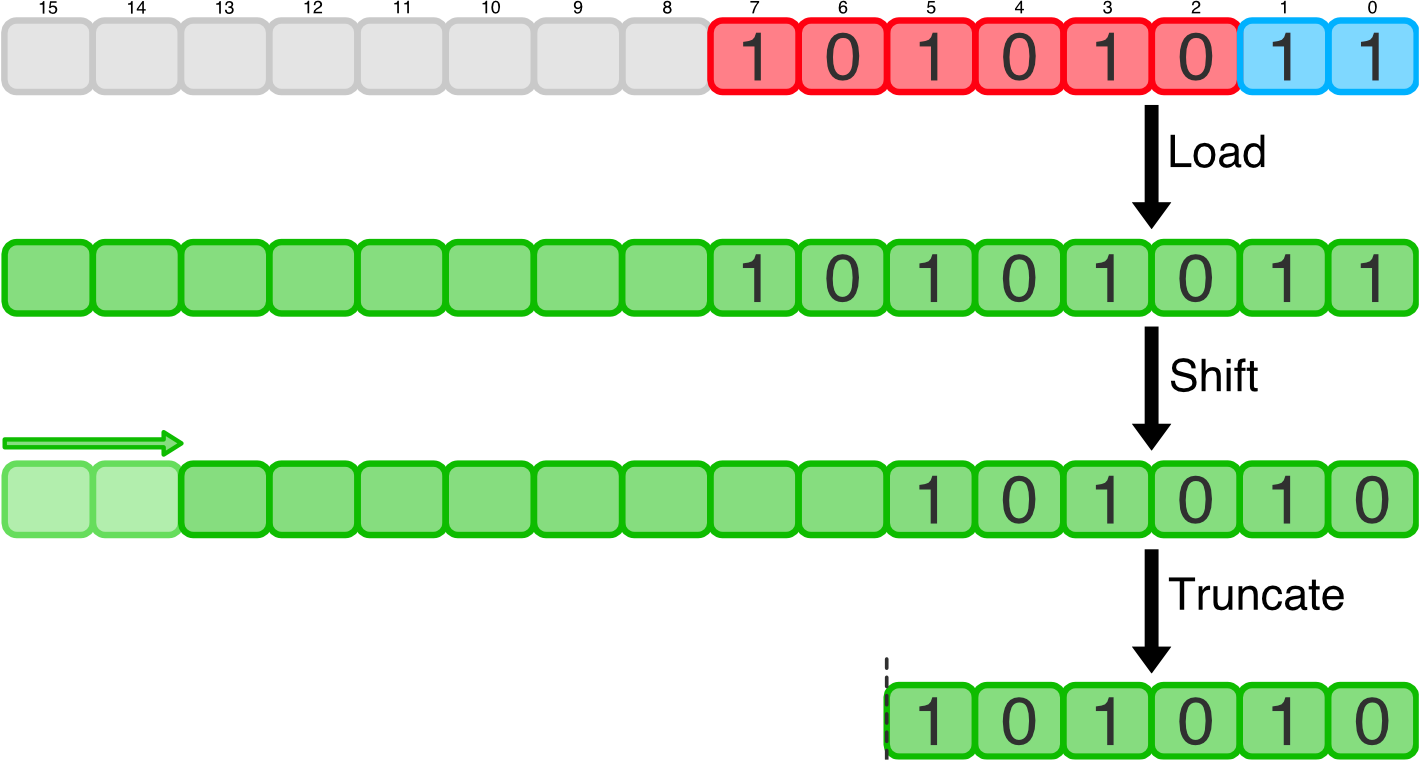
\includegraphics[width=\textwidth]{gfx/Probe.png}
    \caption[<PH> Illustration of the converted probe semantics.]{<PH> Illustration of the converted probe semantics. Here we want to probe an \texttt{i6} sub-signal (red area) of an \texttt{i8} signal (bits $0$
        through $7$). The gray area represents the buffer region allocated for the signal.}
    \label{fig:prb}
\end{figure}

Driving a signal requires us to spawn a new event in the event queue of the simulator, rather than directly update the stored signal value. As mentioned before, we interact with the state through a runtime library, and we do the same here. We use a runtime function, \texttt{drive\_signal}, to take the new value to drive, and spawn a new event after the drive delay, or add the change to an existing event, if one for the given timestamp already exists.

In the case a gating condition is present on the drive, we also generate additional blocks, to conditionally execute or skip the drive based on the gating condition.

A reg operation conditionally drives one value out of a list of triggers and possible values. We can see this operation as a list of comparison blocks, similar to the ones we use for process resumption, leading to a block containing a normal drive operation, which arguments come from the block's arguments. This way we can reuse the drive operation conversion pattern and avoid some redundancy in the pass implementation.

%---

% \subsubsection{others?}


%-------------------------------------------------------------------------------

\subsection{Simulation Trace}
\label{sec:trace}
The simulation trace dump is the main output of a simulation. It lists all changes that occurred on the signals during the simulation. Traditionally, a simulator will work with a trace format similar to \textit{VCD}, the \textit{Variable Change Dump} format, which is also part of the SystemVerilog standard \cite{SV2018}. This format can then be used to visualize waveforms in programs such as \textit{GTKWave} \cite{gtkwave}, but has the downside of not being human-readable by itself, and automated comparison is not trivial (though utilities such as \textit{vcddiff} \cite{vcddiff} exist).

We propose a textual trace dump format, which is both human-readable without the aid of additional software, and easy to compare through widely available tools such as the \textit{diff} command-line tool.


In this textual representation, we use the following syntax:
\mint[showspaces, fontsize=\footnotesize]{c}|<timestamp>  <full-signal-hierarchical-path>  <value>|
\noindent The first element is the full timestamp, reporting the exact time, including delta and epsilon steps separated by one blank space. Next, we report a slash-separated (/) full hierarchical path of the updated signal.
% where we first print the timestamp of the value change, listing the real-time, delta step and epsilon values separated by one space. Next we can find a slash-separated (/) full hierarchical path of the signal, and finally the value the signal assumes at that time-step. The three elements of the entry are separated by two white spaces.
Finally, we print the new value in hexadecimal format, with prefixed by \texttt{0x}, and $0$-padded to the nearest byte. Reason for this is mainly to keep a compact and coherent format throughout the whole trace. But this comes at the cost of not being able to distinguish, for example, an \texttt{i1} signal from an \texttt{i8} signal by purely looking at the trace.

For structured-type signals, we transpose the signal value dump by generating one trace entry for each element of the signal, and appending the respective index to the hierarchical path.

A single signal generates one entry for each instance it is connected to, with the respective hierarchical path. Here we also note that our current implementation, we cannot retrieve the port names in the unit signatures, and we thus have  to use the original name of the signal for all the hierarchical paths of the connected instances, rather than the port names.

A signal generates an entry in the trace only if a drive causes an actual change to the signal value. If a drive occurs, which does not actually change the signal value, it generates no entry in the trace.

Within the same time-step, we define the order for the entries to follow the lexicographical order by the full hierarchical paths. This allows a more normalized and well-formed comparison between traces.

Listing \ref{listing:toggle_trace} shows an example of trace for the first $10$ns of simulation of Listing \ref{listing:mlir_toggle}. Note that all the real-time values are listed in picoseconds. This is because we currently have assigned a static granularity of $1$ps for the simulator and don't perform any further formatting for the time values.

\begin{listing}[ht]
    \caption[An example of \texttt{llhd-sim}'s textual trace.]{An example of the trace generated by simulating the design in Listing \ref{listing:mlir_toggle} for the first $10$ns of execution.}
    \label{listing:toggle_trace}
    \inputminted[
        frame=lines,
        framesep=2mm,
        baselinestretch=1.0,
        bgcolor=lightgray!10,
        fontsize=\footnotesize, linenos
    ]{c}{examples/trace_toggle.txt}
\end{listing}

One of the main downsides of this textual representation of the signal dump is its size. In fact, when simulating full designs, this easily reaches multiple Gigabytes in size, which makes human inspection hard, as files of such size cannot be easily loaded in a text editor. Also, as the amount of signals in the design grows, the information gets too dense for an effective human inspection.

For those reasons, we also propose some variations of this format, that can also be further explored in the future.

\begin{enumerate}
    \item Limit the traced signals to only the ones at the top level of the design. Those are usually the signals owned by the simulated test-bench, and are often the ones of most interest for human inspection. The rationale for this is that the tested circuit can be seen as a “black-box“, and we can infer its correctness by the correctness of its results (the top-level signals).
    \item Merge all sub-steps into their real-time-step, such that only the final state of each signal is present for each time-step. This brings the trace closer to a typical VCD trace, where time sub-steps are not listed. Here we also group all signal changes that occur at the same time-step under only one timestamp, as shown in Listing \ref{listing:merged-syntax}. This allows to identify time-steps more easily when visually inspecting the trace.
    \item Trace only the top-level signals and merge all time sub-steps. This effectively merges the concepts introduced in variations 1. and 2., to further ease visual inspection.
    \item Filter out default-named helper signals. \texttt{moore} often introduces new helper signals during compilation to fully represent the original design. These will not have a name representative of the signal, but are rather given an SSA ID as any other value in the IR. In non-LLHD simulators though, those signals are not represented, as they're not part of the original design. Filtering them out enables us to perform a comparison against SystemVerilog simulators.
\end{enumerate}

% A first variation just limits the traced signals to only the ones at the top level of the design. Those are usually the signals owned by the test-bench that is being simulated, and often the ones of most interest when human interaction is necessary.

% A further variation merges all time sub-steps into their real-time step, as shown in Listing \ref{listing:merged-syntax}. Here we list the timestamp of the current time-step only once, followed by all changes for that step. This brings the trace closer to a typical VCD trace, where only real-time step are represented. This also cuts down on the dump size. Here as for the full trace representation, we can restrict the traced format to only the top level. We can finally filter out all helper signals that are created during the compilation of a design to LLHD (those signals will have a standardized name, in our case \textit{sigN}, where \textit{N} is an integer number).

\begin{listing}[ht]
    \caption{The syntax of the merged textual dump format.}
    \label{listing:merged-syntax}
    \centering
    \begin{minipage}{0.6\textwidth}
        \begin{minted}[fontsize=\footnotesize, showspaces]{c}
<timestamp>
  <full-signal-hierarchical-path>  <value>
  <full-signal-hierarchical-path>  <value>
  ...
            \end{minted}
    \end{minipage}
\end{listing}

We also provide a starting point for a modular tracing infrastructure, with the goal of making it easier to add more formats in the future, such as VCD, to also enable a standard format.


%04-evaluation.tex
\chapter{Evaluation}
\label{ch:eval}

In this chapter, we evaluate the correctness and the performance of our MLIR-based simulator using the same test set used in the LLHD paper~\cite{Schuiki2020}, including a full \textit{Snitch} processor core~\cite{Zaruba2020}. We use \texttt{moore} version $0.6.0$ as the reference compiler to get the SystemVerilog test set in LLHD (with no additional flags active during compilation), paired with Martin Erhart's MLIR writer, to convert the original LLHD syntax to the MLIR syntax. The only manual modification applied to the compiled designs is removing some drives, erroneously inserted by \texttt{moore}, and that would otherwise break the simulation by resetting the affected signal to its default value (\eg, $0$ for integers) after a $0$-time delay. This occurred in the \textit{CDC (Gray)}, \textit{Graycode}, \textit{RR Arbiter}, and \textit{Snitch} examples.

We note that the version of \texttt{moore} we're using doesn't correspond to the latest available version, but it is the most tested, and we can guarantee that the LLHD output it generates is well-formed. When using the latest version ($0.10.0$ at the time of writing), we noticed some discrepancies that could be either due to edge-cases not covered in our simulator or bugs introduced in \texttt{moore} after some major refactorings. We note that in \texttt{moore} version $0.11.0$, released after we generated our evaluation, those discrepancies seem to have been lifted, though a more accurate inspection would be required. All the examples of the test set, as well as the scripts used to generate the evaluations, can also be found on our public testing GitHub repo\footnote{\url{github.com/rodonisi/llhd-extras}}.

%---------------------------------------------------------------------------------------------------

\section{Simulator Correctness}
\label{sec:correctness}
We test for correctness by comparing the trace generated by our simulator for the top-level signals (using the variant 4. of the trace format, described in Section~\ref{sec:trace}) against the one generated by Xilinx's Vivado's simulator~\cite{vivado}, once again only keeping the top-level signals of the design (\ie, the test-bench signals).

To obtain a reliable comparison, we wrote a simple python script to translate the VCD trace generated by Vivado to our textual format (using the \textit{vcdvcd}~\cite{vcdvcd} python module to parse the input VCD file). We then proceed by generating a diff (using the \texttt{diff} command-line tool) of the full trace generated by Vivado, against the full trace we obtain with our simulator.

We remark that since we cannot currently save the port names for the various instance arguments, a comparison of the traces below the top-level becomes a non-trivial task. For the top-level though, where all the signal names are dictated by the original signal names, rather than the port names, we can trivially perform a comparison. Furthermore, by treating the underlying circuit as a “black box“ and observing its output signals, we can still infer the correctness of our simulation, as those signals depend on the correct behavior of the circuit.

We observe that by using LLHD, we are simulating slightly different designs from the original SystemVerilog implementations, due to the lack of a logical type in the current state of LLHD, which is vastly used in SystemVerilog designs. We thus expect slight variations in the simulation traces, but only in cases where a logic type takes either a “don't care“ value (\textit{X}) or a high-impedance value (\textit{Z}). An example can be seen in Listing~\ref{listing:diff-lfsr}.

\begin{listing}
  \lstset{
    escapeinside=||,
    basicstyle=\footnotesize\ttfamily,
    stepnumber=1
  }
  \begin{minipage}{0.45\textwidth}
    \begin{lstlisting}
0ps
  |\textcolor{red}{lfsr\_16bit\_tb/clk\_i  x}|
  |\textcolor{red}{lfsr\_16bit\_tb/en\_i  x}|
  |\textcolor{red}{lfsr\_16bit\_tb/out\_o  x}|
  lfsr_16bit_tb/rst_ni  0x01
1000ps
  lfsr_16bit_tb/out_o  0x0001
  lfsr_16bit_tb/rst_ni  0x00
2000ps
  lfsr_16bit_tb/rst_ni  0x01
...
        \end{lstlisting}
  \end{minipage}
  \hfill
  \begin{minipage}{0.45\textwidth}
    \begin{lstlisting}
0ps
  |\textcolor{ForestGreen}{lfsr\_16bit\_tb/clk\_i  0x00}|
  |\textcolor{ForestGreen}{lfsr\_16bit\_tb/en\_i  0x00}|
  |\textcolor{ForestGreen}{lfsr\_16bit\_tb/out\_o  0x0000}|
  lfsr_16bit_tb/rst_ni  0x01
1000ps
  lfsr_16bit_tb/out_o  0x0001
  lfsr_16bit_tb/rst_ni  0x00
2000ps
  lfsr_16bit_tb/rst_ni  0x01
...
        \end{lstlisting}
  \end{minipage}
  \caption[Side-by-side zoom-in of the LFSR example's diff.]{Side-by-side zoom-in of the LFSR example's diff. Here we can see the case where a \texttt{X} value in Vivado's trace (left) is not reflected in our trace (right), as it cannot currently be represented in LLHD. Note that this excerpt contains all the differences for this example.}
  \label{listing:diff-lfsr}
\end{listing}

A further case where we expect differences is where we don't observe a change due to a previous \texttt{X} or \texttt{Z} value. Listing~\ref{listing:diff-lzc} shows an example where the change at $1000ps$ for signal \textit{cnt\_o} is not reflected in our trace, as the signal is already on that value (at line $3$ of our trace).


\begin{listing}
  \lstset{
    escapeinside=||,
    basicstyle=\footnotesize\ttfamily,
    stepnumber=1
  }
  \begin{minipage}{0.45\textwidth}
    \begin{lstlisting}
0ps
  |\textcolor{red}{lzc\_tb/clk\_i  x}|
  |\textcolor{red}{lzc\_tb/cnt\_o  x}|
  |\textcolor{red}{lzc\_tb/empty\_o  x}|
  |\textcolor{red}{lzc\_tb/in\_i  x}|
  lzc_tb/rst_ni  0x01
1000ps
  |\textcolor{red}{lzc\_tb/cnt\_o  0x0f}|
  lzc_tb/empty_o  0x00
  lzc_tb/in_i  0x0001
  lzc_tb/rst_ni  0x00
2000ps
  lzc_tb/rst_ni  0x01
...
        \end{lstlisting}
  \end{minipage}
  \hfill
  \begin{minipage}{0.45\textwidth}
    \begin{lstlisting}
0ps
  |\textcolor{ForestGreen}{lzc\_tb/clk\_i  0x00}|
  |\textcolor{ForestGreen}{lzc\_tb/cnt\_o  0x0f}|
  |\textcolor{ForestGreen}{lzc\_tb/empty\_o  0x01}|
  |\textcolor{ForestGreen}{lzc\_tb/in\_i  0x0000}|
  lzc_tb/rst_ni  0x01
1000ps

  lzc_tb/empty_o  0x00
  lzc_tb/in_i  0x0001
  lzc_tb/rst_ni  0x00
2000ps
  lzc_tb/rst_ni  0x01
...
        \end{lstlisting}
  \end{minipage}
  \caption[Side-by-side zoom-in of the LZC example's diff.]{Side-by-side zoom-in of the LZC example's diff. Here we can see the case where an update from an \texttt{X} value to some other value is not reflected in our trace, if the signal is already carrying the new value in the LLHD model. Note that this excerpt contains all the differences for this example.}
  \label{listing:diff-lzc}
\end{listing}

The only exception not falling under those cases is in the \textit{Stream Delayer} example, where we can see a mismatch in the value initialization not caused by \texttt{X} values, as shown in Listing~\ref{listing:diff-sd}. By inspecting our full trace, we observe that we initialize those signals to the correct values, but they are driven at a time sub-step of the initial real-time step ($0$ps). We presume that Vivado is merging the initial time sub-steps into the next step, rather than the $0$ps step, as we do. We believe our approach to be correct, since treating the initial step as a special case makes the simulation trace less consistent. An additional toggle to enable this behavior, though, could be added to minimize the discrepancies between the simulation traces if what we believe to be Vivado's approach results in being a common practice in well-established simulators.

\begin{listing}
  \lstset{
    escapeinside=||,
    basicstyle=\footnotesize\ttfamily,
    stepnumber=1
  }
  \begin{minipage}{0.45\textwidth}
    \begin{lstlisting}
0ps
  stream_delay_tb/clk_i  x
  [...]
  |\textcolor{red}{stream\_delay\_tb/ready\_i  0x00}|
  |\textcolor{red}{stream\_delay\_tb/ready\_o  0x00}|
  stream_delay_tb/rst_ni  0x01
  stream_delay_tb/valid_i  0x01
  |\textcolor{red}{stream\_delay\_tb/valid\_o  0x00}|
1000ps
  |\textcolor{red}{stream\_delay\_tb/ready\_i  0x01}|
  |\textcolor{red}{stream\_delay\_tb/ready\_o  0x01}|
  stream_delay_tb/rst_ni  0x00
  |\textcolor{red}{stream\_delay\_tb/valid\_o  0x01}|
2000ps
  stream_delay_tb/rst_ni  0x01
...
        \end{lstlisting}
  \end{minipage}
  \hfill
  \begin{minipage}{0.45\textwidth}
    \begin{lstlisting}
0ps
  stream_delay_tb/clk_i  0x00
  [...]
  |\textcolor{ForestGreen}{stream\_delay\_tb/ready\_i  0x01}|
  |\textcolor{ForestGreen}{stream\_delay\_tb/ready\_o  0x01}|
  stream_delay_tb/rst_ni  0x01
  stream_delay_tb/valid_i  0x01
  |\textcolor{ForestGreen}{stream\_delay\_tb/valid\_o  0x01}|
1000ps


  stream_delay_tb/rst_ni  0x00

2000ps
  stream_delay_tb/rst_ni  0x01
...
        \end{lstlisting}
  \end{minipage}
  \caption[Side-by-side zoom-in of the Stream Delayer example's diff.]{Side-by-side zoom-in of the Stream Delayer example's diff. Here we can see the case where we have an initialization mismatch. Some signal changes have been omitted and replaced by a [...] designation for the sake of readability. Note that this excerpt contains all the differences for this example.}
  \label{listing:diff-sd}
\end{listing}

Considering those cases as exceptions, we can assert that we are generating equivalent (though not equal) simulation traces to Vivado's simulator for our test set. Most notably, for the \textit{Graycode} example, we can generate a $100\%$ matching trace. The \textit{Snitch} processor on the other side is the most complex example, and the one with most differences, but all of them fall under the cases described above. A full listing of the raw \texttt{diff}-generated differentials for all traces can be found in Appendix~\ref{app:diffs}.

%---------------------------------------------------------------------------------------------------

\section{Performance Evaluation}
We evaluate the performance of our simulator by taking the median value over $10$ different runs for each design, as an indication of its average runtime that is not too sensitive to outliers. Also, when we mention average slow-downs/speed-ups, we use the geometric mean as the metric.

We disable the trace generation during performance evaluation. The rationale is that we want to measure the performance of the actual simulation, without the bias introduced by trace processing and possible I/O bounds. For example, the processing required to generate the trace format used in Section~\ref{sec:correctness} sometimes requires alone more than $3$ times the time of the actual simulation in the current implementation. We also consider that a user might not require generating a signal trace dump but might rather be more interested in testing whether a test-bench can simulate without errors or triggering assertions, though we note that such features are not yet implemented in LLHD.

All the reported run-times have been generated by running our simulator in release mode on a Linux machine equipped with an i5 $750$ processor running at $2.67Ghz$, and $8GB$ of RAM. Each series of reports is also generated after a fresh restart.

\begin{table}[ht]
  \centering
  \resizebox{\linewidth}{!}{%
    \begin{tabular}{lcccc}
      \toprule
      \textbf{Design} & \begin{tabular}[c]{@{}l@{}}\textbf{MLIR-based}\\\textbf{Simulator [s]*}\end{tabular} & \begin{tabular}[c]{@{}l@{}}\textbf{LLHD Reference }\\\textbf{Simulator [s]*}\end{tabular} & \textbf{LLHD Blaze}~ \textbf{[s]} & \textbf{Vivado [s]} \\
      \toprule
      CDC (Gray)      & 421.80                    & 4894.94                   & 16.55                             & 12.00               \\
      CDC (strobe)    & 622.75                    & 5132.95                   & 16.10                             & 16.00               \\
      FIFO Queue      & 140.22                    & 2324.60                   & 11.77                             & 5.00                \\
      FIR Filter      & 746.35                    & 14807.50                  & 17.97                             & 33.00               \\
      Graycode        & 222.60                    & 14628.93                  & 9.78                              & 23.00               \\
      LFSR            & 636.52                    & 7080.40                   & 25.20                             & 37.00               \\
      LZC             & 155.63                    & 31207.36                  & 5.86                              & 8.00                \\
      RR Arbiter      & 1062.82                   & 84072.45                  & 17.55                             & 75.50               \\
      Snitch          & 382.53                    & 6721.92                   & 48.53                             & 4.81 **             \\
      Stream Delayer  & 139.44                    & 1136.31                   & 8.72                              & 2.84 **             \\
      \bottomrule
    \end{tabular}
  }

  \caption[Comparison of simulation timings for our first simulator prototype.]{Comparison of the time required to simulate the design of our test set on various simulators. All time values are reported in seconds and obtained by summing the \textit{user} and \textit{system} values reported by the \textit{time} command-line utility, or, in Vivado's case, the \textit{elapsed} value reported on simulation completition. \\ * Due to the amount of time required by the LLHD reference simulator, the timings are reported for only one run. \\ ** Due to Vivado not reporting the simulation time after the completition for this case, we fell back to using the “\mintinline{Shell}{time {run all}}“ command. This command otherwise made Vivado often crash for longer simulations, which is why we only use it as a fall-back.}
  \label{tab:timings_compare}
\end{table}

Table~\ref{tab:timings_compare} lists the median timings we obtain with our first prototype of the simulator that can run all the examples from our test set. As a reference, we compare the performance we obtain against the LLHD reference simulator\footnote{Run with no additional flags.}, the LLHD Blaze simulator\footnote{Run with no additional flags.}, and the Vivado simulator\footnote{Always running a fresh simulation through the \mintinline{Shell}{run all} TCL command from the Vivado IDE.}. A full and raw listing of the timing results used to generate this evaluation can be found in Appendix~\ref{app:timings}.

We observe that our simulator is nowhere near obtaining competitive performance when compared against both a commercial simulator and LLHD Blaze (which implements a very similar approach to ours). In particular, our performance is on average $26$ times slower than Vivado's simulator.

In table \ref{tab:time_detail0} we explore a more detailed view of the time spent in various stages of the simulation. Once again the listed values are averaged over multiple executions of the simulator, and full listings for each example can be found in Appendix \ref{app:timings}.

\begin{table}[ht]
  \centering
  \resizebox{\linewidth}{!}{%
    \begin{tabular}{lcccccc}
      \toprule
      \textbf{Design} & \textbf{Total [s]} & \begin{tabular}[c]{@{}l@{}}\textbf{Init}\\\textbf{phase}\end{tabular} & \begin{tabular}[c]{@{}l@{}}\textbf{Allocation}\\\textbf{phase}\end{tabular} & \begin{tabular}[c]{@{}l@{}}\textbf{Signals}\\\textbf{update}\end{tabular} & \begin{tabular}[c]{@{}l@{}}\textbf{Instances}\\\textbf{execution}\end{tabular} & \textbf{Remainder} \\
      \toprule
      CDC (Gray)      & 421.80             & 0\%                       & 0\%                        & 12.80\%                    & 71.48\%                    & 15.72\%            \\
      CDC (strobe)    & 622.75             & 0\%                       & 0\%                        & 10.36\%                    & 75.15\%                    & 14.49\%            \\
      FIFO Queue      & 140.22             & 0\%                       & 0\%                        & 12.12\%                    & 72.39\%                    & 15.49\%            \\
      FIR Filter      & 746.35             & 0\%                       & 0\%                        & 10.05\%                    & 77.98\%                    & 11.97\%            \\
      Graycode        & 222.60             & 0\%                       & 0\%                        & 7.64\%                     & 81.99\%                    & 10.38\%            \\
      LFSR            & 636.52             & 0\%                       & 0\%                        & 10.05\%                    & 79.81\%                    & 10.14\%            \\
      LZC             & 155.63             & 0\%                       & 0\%                        & 10.92\%                    & 76.78\%                    & 12.29\%            \\
      RR Arbiter      & 1062.82            & 0\%                       & 0\%                        & 13.08\%                    & 67.18\%                    & 19.74\%            \\
      Snitch          & 382.53             & 0\%                       & 0\%                        & 11.76\%                    & 67.05\%                    & 20.92\%            \\
      Stream Delayer  & 139.44             & 0\%                       & 0\%                        & 10.04\%                    & 73.15\%                    & 16.81\%            \\
      \bottomrule
    \end{tabular}
  }
  \caption[Detailed performance evaluation of the MLIR-based simulator]{Detailed performance evaluation of the MLIR-based simulator. The \textit{Total} column indicates the total time required to simulate the design from start to end, as reported by the \texttt{time} command-line tool. The remaining columns report the overall percentage of the time spent in that simulation phase. The \textit{Init phase} column includes initializing the state structures, converting the LLHD module to the LLVM dialect, and initializing the JIT compiler. The \textit{Allocation phase} includes executing the generated initialization function. The \textit{Signals update} column includes processing and applying the scheduled updates. The \textit{Remainder} metric reports the percentage of time spent in stages we do not track, including constructing and destroying the simulator, iterating over, and popping the event queue.}
  \label{tab:time_detail0}
\end{table}

We recognize our first prototype prioritized correctness over performance, and as such many of the used data structures and approaches are far from being optimal. Though, we can see an interesting result in the initialization times, where we see the negligible impact of MLIR applying the LLHD-to-LLVM conversion pass (part of the \textit{init phase} metric), as well as the execution of the generated initialization function (\textit{allocation phase} metric). In both cases, the total time required rounds down to $0\%$ of the total simulation time during the formatting of the results. We also see that a great majority of the required simulation time resides in the execution of the various instances. Due to time constraints, we were not able to bring major changes targeted at improving performance, but we observe that some performance optimizations include some low-hanging fruits.

By inspecting the simulator execution with a profiling tool, \texttt{perf}, we get a clearer picture of where we are losing performance. We see that most of the time is spent allocating and deallocating memory for the simulator queue and state-keeping structures. Also, we note that the execution of our lowered LLHD code takes a negligible amount of time (generally around $1$-$2\%$).

Given the profiling results, we applied the following changes, achieving the timing results listed in Table \ref{tab:time_detail1}:

\begin{enumerate}
  \item An overall cleanup of the code and replacement of basic data structures with more efficient implementations, \eg, using LLVM \texttt{SmallVector} instead of standard vectors (where fit).
  \item Initially, we were executing the units through the JIT engine's \texttt{invoke} function. Looking up the compiled function pointers through the JIT compiler turns out to be very expensive, so we switched to storing the compiled function pointers in the instance structures, making them readily available when needed.
  \item We used to map instances to the respective structures by name, requiring us to perform lots of string allocations and comparisons when iterating over the wakeup queue. We thus switched to an integer indexing, more similar to what we were already doing with signals, dramatically cutting down on strings usage.
  \item We observe that the number of events present at the same time in the event queue is fairly small, usually between $2$ and $6$. Given this, we can change the event queue to be a simple, unsorted vector, where we search for the earliest slot in each cycle instead of sorting the queue for each drive. Furthermore, this allows us to reuse the already allocated slots instead of popping and destroying them, significantly cutting down the allocation/deallocation times. We applied the same approach to the slot change buffers, replacing the signal-to-changes map structure with a vector of index-change pairs, and reusing the buffers instead of allocating new ones each time. This also required slightly reworking the signal processing phase, to ensure no additional trace entries and instance wakeups get triggered.
  \item Initially, we used to search through the whole event queue for an existing slot with the given timestamp, for each drive. We avoid redundant iteration over the queue when performing a drive, by:
        \begin{enumerate}
          \item Keeping track of the index of the current earliest event (the \textit{top} of the queue), such that multiple drives to the “next event“ can be directly added to the correct slot without any searching. This could happen, for example, when all bits of a signal are driven independently with the same delay.
          \item If a drive has a timestamp earlier than the current top of the queue, it cannot be part of an existing slot, otherwise it would be the top of the queue. In this case, we directly create a new slot and update the current top index.
          \item If a drive has a timestamp later than the current top, a slot for that event could already be present in the queue. In this case, we need to search the queue for an existing slot and create a new slot if none is found.
        \end{enumerate}
\end{enumerate}

\begin{table}[ht]
  \centering
  \resizebox{\linewidth}{!}{%
    \begin{tabular}{lcccccc}
      \toprule
      \textbf{Design} & \textbf{Total [s]} & \begin{tabular}[c]{@{}l@{}}\textbf{Init}\\\textbf{phase}\end{tabular} & \begin{tabular}[c]{@{}l@{}}\textbf{Allocation}\\\textbf{phase}\end{tabular} & \begin{tabular}[c]{@{}l@{}}\textbf{Signals}\\\textbf{update}\end{tabular} & \begin{tabular}[c]{@{}l@{}}\textbf{Instances}\\\textbf{execution}\end{tabular} & \textbf{Remainder} \\
      \toprule
      CDC (Gray)      & 36.15              & 0\%                        & 0\%                        & 27.66\%                    & 47.02\%                    & 25.32\%            \\
      CDC (strobe)    & 44.65              & 0\%                        & 0\%                        & 29.11\%                    & 51.51\%                    & 19.37\%            \\
      FIFO Queue      & 11.65              & 0\%                        & 0\%                        & 25.76\%                    & 42.93\%                    & 31.31\%            \\
      FIR Filter      & 72.96              & 0\%                        & 0\%                        & 23.30\%                    & 53.46\%                    & 23.24\%            \\
      Graycode        & 19.24              & 0\%                        & 0\%                        & 20.79\%                    & 57.18\%                    & 22.02\%            \\
      LFSR            & 36.87              & 0\%                        & 0\%                        & 21.70\%                    & 46.11\%                    & 32.19\%            \\
      LZC             & 33.04              & 0\%                        & 0\%                        & 18.16\%                    & 54.48\%                    & 27.36\%            \\
      RR Arbiter      & 199.22             & 0\%                        & 0\%                        & 23.84\%                    & 51.70\%                    & 24.46\%            \\
      Snitch          & 66.11              & 0\%                        & 0\%                        & 21.18\%                    & 46.89\%                    & 31.93\%            \\
      Stream Delayer  & 11.59              & 0\%                        & 0\%                        & 25.89\%                    & 43.15\%                    & 30.96\%            \\
      \bottomrule
    \end{tabular}
  }
  \caption[Detailed performance evaluation of the optimized MLIR-based simulator.]{Detailed performance evaluation of the optimized MLIR-based simulator. For the specification of the reported values please refer to the description of Table \ref{tab:time_detail0}.}
  \label{tab:time_detail1}
\end{table}

We see a significant performance improvement with the changes we applied. Also, given the faster simulation speeds we can obtain, we now observe our timing method introduces significant overhead, as high as $40\%$ in the worst case, due to the millions of calls into the \textit{C++} \texttt{std::chrono} library. These overheads where of negligible impact on our first, slower implementation. Tracking the simulation timing at this granularity is an optional feature, mostly targeted at debugging the simulator and not of general interest in a simulation. We thus provide a final timing report in Table~\ref{tab:timings_compare1}, where we do not use any additional flags other than the required \textit{root} entity specification, and disabling the trace generation. Here we also report the timings of the reference simulators as in Table \ref{tab:timings_compare}, to make it easier for the reader to compare the new timings against the reference simulators.

\begin{table}[ht]
  \centering
  \resizebox{\linewidth}{!}{%
    \begin{tabular}{lcccc}
      \toprule
      \textbf{Design} & \begin{tabular}[c]{@{}l@{}}\textbf{MLIR-based}\\\textbf{Simulator [s]*}\end{tabular} & \begin{tabular}[c]{@{}l@{}}\textbf{LLHD Reference }\\\textbf{Simulator [s]*}\end{tabular} & \textbf{LLHD Blaze}~ \textbf{[s]} & \textbf{Vivado [s]} \\
      \toprule
      CDC (Gray)      & 32.84                      & 4894.94                    & 16.55                             & 12.00               \\
      CDC (strobe)    & 39.52                      & 5132.95                    & 16.10                             & 16.00               \\
      FIFO Queue      & 10.19                      & 2324.60                    & 11.77                             & 5.00                \\
      FIR Filter      & 63.76                      & 14807.50                   & 17.97                             & 33.00               \\
      Graycode        & 16.53                      & 14628.93                   & 9.78                              & 23.00               \\
      LFSR            & 26.34                      & 7080.40                    & 25.20                             & 37.00               \\
      LZC             & 31.25                      & 31207.36                   & 5.86                              & 8.00                \\
      RR Arbiter      & 190.17                     & 84072.45                   & 17.55                             & 75.50               \\
      Snitch          & 64.10                      & 6721.92                    & 48.53                             & 4.81                \\
      Stream Delayer  & 10.52                      & 1136.31                    & 8.72                              & 2.84                \\
      \bottomrule
    \end{tabular}
  }
  \caption[Performance comparison with the optimized MLIR-based simulator.]{Performance comparison with the optimized MLIR-based simulator. The values for the reference simulators are reported as in Figure \ref{tab:timings_compare}.}
  \label{tab:timings_compare1}
\end{table}

We observe that we can now surpass the performance of Vivado's simulator in two cases and LLHD-Blaze's performance in one case. We though notice that our simulator still does not scale as well as Vivado on more complex examples, \eg, our simulator runs $13.3$ times slower than Vivado for the \textit{Snitch} example, compared to the \textit{Graycode} and \textit{LFSR} examples, which both run $1.4$ times faster.

Profiling of the execution shows a great majority of the time is still used creating new events ($\sim$$40\%$) and processing the events ($\sim$$25\%$), while the execution of JIT-compiled instances' themselves still takes a relatively small amount of the total execution ($\sim$$10\%$). We are confident that further optimization of the current implementation could bring this sequential approach to truly competitive performance.

%05-conclusion.tex

\chapter{Conclusion}
With this thesis, we showed that LLHD is fully representable in MLIR (and that our representation is correct) by defining an LLHD dialect and correctly simulating various real-world designs represented in it.
Furthermore, our first implementation of the MLIR-based simulator already comes close to competitive performance. In particular, our simulator manages to surpass a well-established commercial simulator for some test cases, running up to $1.5$ times faster and otherwise only $3.2$ times slower on average. This while being a very young and poorly optimized sequential implementation.
We also showed that the performance losses in our implementation mainly reside in the runtime library and simulator engine, and not in the execution of the lowered LLHD code, making the simulator a good optimization target with high speed-up potential. The small set of optimization we could implement already shows the massive performance speed-up potential present in our simulator. We are confident that further exploration of LLHD-based simulation could enable a new and open-source standard in HDL simulation and verification.

%---------------------------------------------------------------------------------------------------

\section{Related Work}
Various open-source HDL simulators exist on the market, but, to our knowledge, none has support for the SystemVerilog standard as vast as LLHD, or does not support SystemVerilog or VHDL at all. Here we list some of the most popular and well-documented open-source alternatives available.

%-------------------------------------------------------------------------------

\subsection{Verilator}
\textit{Verilator} \cite{verilator} is a popular open-source simulator. It profits from high simulation speeds by compiling SystemVerilog designs into single- or multi-threaded \textit{C++} code, though, mainly synthesizable constructs are accepted. This means that SystemVerilog test-benches cannot be simulated using Verilator as they generally contain unsynthesizable constructs. Instead, the user is expected to write a \textit{C++/SystemC} wrapper around the design under test, (re-)implementing the test-bench. An important distinction that sets Verilator apart from our approach is that Verilator does not have any support for explicit delays, often throwing an error if one is encountered, or otherwise ignoring it.

% \section{Lifting}
% The Lifting \cite{Bosio2008} offers both behavioral and fault simulation, though it is more focused on the latter.

%-------------------------------------------------------------------------------

\subsection{SystemC and Cascade}
\textit{SystemC} \cite{systemc} and \textit{Cascade} \cite{Grossman2013}  bothe define a \textit{C++} library used to model hardware designs. The \textit{C++} constructs can then be used as simulation interfaces, and usually be compiled into an executable performing the simulation.

These approaches, though, do not interface with SystemVerilog or VHDL, but rather expect the designs to be directly implemented through the \textit{C++} constructs. For example, SystemC is often considered as a standalone HDL (though it is \textit{C++}) and even takes a spot in Wikipedia's list of HDLs\footnote{\url{https://en.wikipedia.org/wiki/Hardware_description_language\#Examples_of_HDLs}}.

Cascade also takes a cycle-based simulation approach, in contrast to both our approach and SystemC's. This means that simulation state updates are no longer processed on an event-basis, where the time granularity is defined by the events themselves, but rather on fixed clock cycles. Furthermore, Cascade offers Verilog co-simulation, but this is mainly to support Verilog test-benches, rather than entire Verilog designs.

%-------------------------------------------------------------------------------

\subsection{Icarus Verilog and OSS CVC}
\textit{Icarus Verilog} \cite{icarus} and the \textit{OSS CVC} Verilog compiler \cite{Meyer2016}, to our knowledge, are the two open-source simulation toolchains that most closely resemble our simulation approach.

Icarus Verilog is an open-source implementation of Verilog, mainly focusing on simulation, but also providing support for synthesis. Different from LLHD, though, it focuses on the IEEE Std 1364-2005 Verilog standard \cite{V2006}, with only limited support for the SystemVerilog standard. Most notably, it does not accept any of the examples from our test set. It is otherwise very similar to LLHD's workflow: the input design is first compiled to an intermediate representation, called \textit{vpp}, which can be used for either simulation (through the \textit{vpp} tool) or synthesis.

OSS CVC, on the other hand, compiles Verilog designs directly to x86 machine code and then uses an event-driven approach to simulate the input design. As for Icarus Verilog though, it is only limited to the IEEE Std 1364-2005 Verilog standard, precluding the use of the higher-level SystemVerilog extensions.

%---------------------------------------------------------------------------------------------------

\section{Future Work}
We think our first implementation opens up many interesting research questions that could be explored in the future, including:

\begin{itemize}
  \item Though initially planned for this thesis, we did not manage to explore what speed-ups we could obtain through a multi-threaded simulation approach. Considering that a significant amount of time in our simulation is spent in creating events, we think adopting a simple  \textit{Centralized-Queue} algorithm \cite{Ashenden1994} could already bring significant performance improvements, by splitting that phase over multiple threads.
  \item We did not explore what optimizations and performance improvements other MLIR dialects and transformations could enable, but rather directly lower from LLHD to the LLVM dialect, only optimizing the generated LLVM IR code through the provided “O“ flags. Especially with the rise of the CIRCT project, and other hardware-targeted dialects, it will pose an interesting question of what performance improvements they could bring to LLHD simulation.
  \item Introducing static analysis of the input design could potentially bring significant performance improvements. For example, the input design could be analyzed to preemptively allocate the memory buffers necessary to store the various signal updates in the event queue, reducing the costs of dynamic memory allocation. Further analysis could potentially completely avoid the execution of parts of the input design that have no visible effects on the execution. \Eg, consider two processes $A$ and $B$. If $B$'s signal updates always obscure $A$'s updates, then $A$ does not affect the overall behavior of the design, and its execution can be avoided.
  \item Both the LLHD dialect and LLVM dialect mapping are not complete. \Eg, introducing support for logic types would enable us to generate $100\%$ matching traces when compared against commercial simulators.
        % \item We provided only a limited comparison of our performance results, only comparing it against one commercial simulator. This choice was mainly due to the missing availability of other commercial tools on our testing machine and time constraints. More complete benchmarking and comparison of the current and future implementations of our simulator against a broader range of commercial simulators could give us a clearer picture of the potential of this HDL simulation approach.
\end{itemize}





\cleardoublepage % Empty page before the start of the next part

%----------------------------------------------------------------------------------------
%	THESIS CONTENT - APPENDICES
%----------------------------------------------------------------------------------------

\appendix

% \part{Appendix} % New part of the thesis for the appendix

\chapter{Diff Listings}
\label{app:diffs}

This appendix contains the full listing of the differences obtain when running the \texttt{diff} utility on the trace generated through Vivado's simulator (on the left, lines starting with “\texttt{<}“) against the trace generated with our MLIR-based simulator (on the right, lines starting with “\texttt{>}“). Note that a listing for the \textit{Graycode} example is not provided, as no diff is generated for that example. Also, due to a large amount of variable “don't care“ values (\texttt{x}) present in the Snitch's trace, we only list the diff for the first $50$ns for that example, but we note that all the remaining changes follow the same pattern as the ones we show, where the differences are all due to the signal \texttt{data\_qdata\_o} receiving \texttt{x} payloads.

\begin{listing}[H]
    \inputminted[
        frame=lines,
        framesep=2mm,
        baselinestretch=1.0,
        % bgcolor=lightgray!10,
        fontsize=\footnotesize, linenos
    ]{c}{diffs/diff-cdc_fifo_gray_tb.txt}
    \caption{Full \texttt{diff} listing for the CDC (Gray) example.}
\end{listing}

\begin{listing}[H]
    \inputminted[
        frame=lines,
        framesep=2mm,
        baselinestretch=1.0,
        % bgcolor=lightgray!10,
        fontsize=\footnotesize, linenos
    ]{c}{diffs/diff-cdc_2phase_tb.txt}
    \caption{Full \texttt{diff} listing for the CDC (strobe) example.}
\end{listing}

\begin{listing}[H]
    \inputminted[
        frame=lines,
        framesep=2mm,
        baselinestretch=1.0,
        % bgcolor=lightgray!10,
        fontsize=\footnotesize, linenos
    ]{c}{diffs/diff-fifo_v3_tb.txt}
    \caption{Full \texttt{diff} listing for the FIFO Queue example.}
\end{listing}

\begin{listing}[H]
    \inputminted[
        frame=lines,
        framesep=2mm,
        baselinestretch=1.0,
        % bgcolor=lightgray!10,
        fontsize=\footnotesize, linenos
    ]{c}{diffs/diff-fir_tb.txt}
    \caption{Full \texttt{diff} listing for the FIR example.}
\end{listing}

\begin{listing}[H]
    \inputminted[
        frame=lines,
        framesep=2mm,
        baselinestretch=1.0,
        % bgcolor=lightgray!10,
        fontsize=\footnotesize, linenos
    ]{c}{diffs/diff-lfsr_16bit_tb.txt}
    \caption{Full \texttt{diff} listing for the LFSR example.}
\end{listing}

\begin{listing}[H]
    \inputminted[
        frame=lines,
        framesep=2mm,
        baselinestretch=1.0,
        % bgcolor=lightgray!10,
        fontsize=\footnotesize, linenos
    ]{c}{diffs/diff-lzc_tb.txt}
    \caption{Full \texttt{diff} listing for the LZC example.}
\end{listing}

\begin{listing}[H]
    \inputminted[
        frame=lines,
        framesep=2mm,
        baselinestretch=1.0,
        % bgcolor=lightgray!10,
        fontsize=\footnotesize, linenos
    ]{c}{diffs/diff-rr_arb_tree_tb.txt}
    \caption{Full \texttt{diff} listing for the RR Arbiter example.}
\end{listing}


\begin{listing}[H]
    \inputminted[
        frame=lines,
        framesep=2mm,
        baselinestretch=1.0,
        % bgcolor=lightgray!10,
        fontsize=\footnotesize, linenos
    ]{c}{diffs/diff-snitch_tb.txt}
    \caption[Full \texttt{diff} listing for the Snitch example.]{Full \texttt{diff} listing for the Snitch example. Note that due to the amount of variable don't care (\texttt{x} values, we only report the differences for the first $50$ns of simulation for this example. We also note that the remaining differences follow the pattern shown in this listing, and all differ either because of an \texttt{x} value, or are a consequence of one of those values.}
\end{listing}

\begin{listing}[H]
    \inputminted[
        frame=lines,
        framesep=2mm,
        baselinestretch=1.0,
        % bgcolor=lightgray!10,
        fontsize=\footnotesize, linenos
    ]{c}{diffs/diff-stream_delay_tb.txt}
    \caption{Full \texttt{diff} listing for the Stream Delayer example.}
\end{listing} % Appendix A
\chapter{Timing Tables}
\label{app:timings}
This appendix contains the raw timing results, which averages are reported in Chapter~\ref{ch:eval}. For our MLIR-based simulator, we also report detailed timings for the various stages of the simulation, for each example and both the first prototype and the (slightly optimized) second prototype.

\section{Reference Simulators Timings}

\begin{table}[ht]
    \centering
    \begin{tabular}{ll}
        \toprule
        \textbf{Design} & \textbf{1} \\
        \toprule
        CDC (Gray)      & 4894.94    \\
        CDC (strobe)    & 5132.95    \\
        FIFO Queue      & 2324.60    \\
        FIR Filter      & 14807.50   \\
        Graycode        & 14628.93   \\
        LFSR            & 7080.40    \\
        LZC             & 31207.36   \\
        RR Arbiter      & 84072.45   \\
        Snitch          & 6721.92    \\
        Stream Delayer  & 1136.31    \\
        \bottomrule
    \end{tabular}
    \caption{Raw timings table for LLHD-Sim.}
\end{table}

\begin{table}[h]
    \centering

    \resizebox{\linewidth}{!}{%
        \begin{tabular}{lllllllllll}
            \toprule
            \textbf{Design}  & \textbf{1} & \textbf{2} & \textbf{3} & \textbf{4} & \textbf{5} & \textbf{6} & \textbf{7} & \textbf{8} & \textbf{9} & \textbf{10} \\
            \toprule
            CDC (Gray)       & 12         & 12         & 12         & 12         & 12         & 12         & 12         & 12         & 12         & 12          \\
            CDC (strobe)     & 16         & 16         & 16         & 16         & 16         & 16         & 16         & 16         & 16         & 17          \\
            FIFO Queue       & 5          & 6          & 5          & 6          & 5          & 5          & 6          & 5          & 5          & 5           \\
            FIR Filter       & 33         & 33         & 33         & 33         & 34         & 33         & 33         & 33         & 33         & 33          \\
            Graycode         & 23         & 23         & 23         & 23         & 23         & 23         & 23         & 23         & 23         & 23          \\
            LFSR             & 37         & 37         & 37         & 38         & 38         & 37         & 37         & 37         & 37         & 37          \\
            LZC              & 8          & 8          & 8          & 8          & 8          & 8          & 8          & 8          & 8          & 8           \\
            RR Arbiter       & 76         & 76         & 76         & 76         & 75         & 76         & 75         & 75         & 75         & 75          \\
            Snitch *         & 4.81       & 4.83       & 4.81       & 4.79       & 4.77       & 4.81       & 4.76       & 4.81       & 4.81       & 4.76        \\
            Stream Delayer * & 2.95       & 2.86       & 2.83       & 2.82       & 2.82       & 2.84       & 2.83       & 2.85       & 2.87       & 2.84        \\
            \bottomrule
        \end{tabular}
    }
    \caption{Raw timings table for Vivado's simulator. \\ * The timings for the \textit{Snitch} and \textit{Stream Delayer} examples have been measured using the \textit{TCL time} command, due to Vivado not reporting the simulation times for those cases. Using the same command for the remainder of the examples would also make Vivado crash on our testing machine, so we kept the default times reported on simulation completition.}
\end{table}

\begin{table}[h]
    \centering
    \resizebox{\linewidth}{!}{%
        \begin{tabular}{lllllllllll}
            \toprule
            \textbf{Design} & \textbf{1} & \textbf{2} & \textbf{3} & \textbf{4} & \textbf{5} & \textbf{6} & \textbf{7} & \textbf{8} & \textbf{9} & \textbf{10} \\
            \toprule
            CDC (Gray)      & 16.37      & 16.80      & 16.43      & 16.51      & 16.75      & 16.71      & 16.59      & 16.31      & 16.56      & 16.53       \\
            CDC (strobe)    & 16.27      & 15.98      & 16.24      & 16.68      & 15.85      & 16.04      & 16.15      & 16.18      & 15.97      & 15.91       \\
            FIFO Queue      & 11.82      & 11.86      & 11.79      & 11.75      & 11.68      & 11.88      & 11.70      & 11.75      & 11.69      & 11.79       \\
            FIR Filter      & 17.81      & 18.12      & 17.76      & 17.91      & 18.03      & 17.97      & 18.23      & 17.97      & 17.97      & 18.19       \\
            Graycode        & 9.85       & 9.75       & 9.74       & 9.80       & 9.81       & 9.74       & 9.70       & 9.80       & 9.95       & 9.75        \\
            LFSR            & 25.18      & 25.12      & 25.56      & 25.16      & 25.32      & 24.34      & 25.22      & 25.75      & 25.10      & 25.24       \\
            LZC             & 5.85       & 5.91       & 5.85       & 5.80       & 5.83       & 5.92       & 5.87       & 5.92       & 5.84       & 5.88        \\
            RR Arbiter      & 17.64      & 17.70      & 17.82      & 17.66      & 17.53      & 17.51      & 17.39      & 17.39      & 17.57      & 17.31       \\
            Snitch          & 49.08      & 48.52      & 48.47      & 48.39      & 48.55      & 48.66      & 48.16      & 48.76      & 48.33      & 48.53       \\
            Stream Delayer  & 8.74       & 8.70       & 8.64       & 8.65       & 8.69       & 8.91       & 8.85       & 8.69       & 8.80       & 8.74        \\
            \bottomrule
        \end{tabular}
    }
    \caption{Raw timings table for the LLHD Blaze simulator.}
\end{table}

%---------------------------------------------------------------------------------------------------

\clearpage
\section{MLIR-Based Simulator Timings}
\subsection{First Prototype}

\begin{table}[h]
    \centering
    \resizebox{\linewidth}{!}{%
        \begin{tabular}{cccccc}
            \toprule
            \textbf{Total [s]} & \begin{tabular}[c]{@{}l@{}}\textbf{Engine}\\\textbf{init [s]}\end{tabular} & \begin{tabular}[c]{@{}l@{}}\textbf{Allocation}\\\textbf{phase [s]}\end{tabular} & \begin{tabular}[c]{@{}l@{}}\textbf{Signals}\\\textbf{update [s]}\end{tabular} & \begin{tabular}[c]{@{}l@{}}\textbf{Instances}\\\textbf{execution [s]}\end{tabular} & \textbf{Remainder [s]} \\
            \toprule
            420.74             & 0                         & 0                         & 54                        & 301                       & 65.74                  \\
            423.88             & 0                         & 0                         & 54                        & 302                       & 67.88                  \\
            418.7              & 0                         & 0                         & 54                        & 301                       & 63.70                  \\
            415.07             & 0                         & 0                         & 55                        & 296                       & 64.07                  \\
            422.53             & 0                         & 0                         & 55                        & 302                       & 65.53                  \\
            421.12             & 0                         & 0                         & 54                        & 301                       & 66.12                  \\
            423.83             & 0                         & 0                         & 54                        & 304                       & 65.83                  \\
            435.63             & 0                         & 0                         & 57                        & 310                       & 68.63                  \\
            422.47             & 0                         & 0                         & 54                        & 303                       & 65.47                  \\
            415.54             & 0                         & 0                         & 54                        & 296                       & 65.54                  \\
            \bottomrule
        \end{tabular}
    }
    \caption{Detailed timings reports for the CDC (Gray) example.}
\end{table}

\begin{table}[h]
    \centering
    \resizebox{\linewidth}{!}{%
        \begin{tabular}{cccccc}
            \toprule
            \textbf{Total [s]} & \begin{tabular}[c]{@{}l@{}}\textbf{Engine}\\\textbf{init [s]}\end{tabular} & \begin{tabular}[c]{@{}l@{}}\textbf{Allocation}\\\textbf{phase [s]}\end{tabular} & \begin{tabular}[c]{@{}l@{}}\textbf{Signals}\\\textbf{~[s]}\end{tabular} & \begin{tabular}[c]{@{}l@{}}\textbf{Instances}\\\textbf{execution [s]}\end{tabular} & \textbf{Remainder [s]} \\
            \toprule
            614.45             & 0                         & 0                         & 64                         & 465                        & 85.45                  \\
            626.65             & 0                         & 0                         & 66                         & 473                        & 87.65                  \\
            624.26             & 0                         & 0                         & 64                         & 472                        & 88.26                  \\
            621.23             & 0                         & 0                         & 65                         & 469                        & 87.23                  \\
            635.09             & 0                         & 0                         & 65                         & 481                        & 89.09                  \\
            612.59             & 0                         & 0                         & 64                         & 461                        & 87.59                  \\
            617.6              & 0                         & 0                         & 64                         & 467                        & 86.6                   \\
            631.92             & 0                         & 0                         & 66                         & 462                        & 103.92                 \\
            627.38             & 0                         & 0                         & 66                         & 472                        & 89.38                  \\
            619.48             & 0                         & 0                         & 63                         & 467                        & 89.48                  \\
            \bottomrule
        \end{tabular}
    }
    \caption{Detailed timings reports for the CDC (strobe) example.}
\end{table}


\begin{table}[h]
    \centering
    \resizebox{\linewidth}{!}{%
        \begin{tabular}{cccccc}
            \toprule
            \textbf{Total [s]} & \begin{tabular}[c]{@{}l@{}}\textbf{Engine}\\\textbf{init [s]}\end{tabular} & \begin{tabular}[c]{@{}l@{}}\textbf{Allocation}\\\textbf{phase [s]}\end{tabular} & \begin{tabular}[c]{@{}l@{}}\textbf{Signals}\\\textbf{update [s]}\end{tabular} & \begin{tabular}[c]{@{}l@{}}\textbf{Instances}\\\textbf{execution [s]}\end{tabular} & \textbf{Remainder [s]} \\
            \toprule
            139.88             & 0                          & 0                          & 17                         & 102                        & 20.88                  \\
            140.56             & 0                          & 0                          & 18                         & 101                        & 21.56                  \\
            142.13             & 0                          & 0                          & 17                         & 102                        & 23.13                  \\
            143.1              & 0                          & 0                          & 17                         & 104                        & 22.1                   \\
            142.38             & 0                          & 0                          & 18                         & 103                        & 21.38                  \\
            138.80             & 0                          & 0                          & 17                         & 101                        & 20.8                   \\
            139.62             & 0                          & 0                          & 17                         & 101                        & 21.62                  \\
            139.78             & 0                          & 0                          & 17                         & 101                        & 21.78                  \\
            138.23             & 0                          & 0                          & 17                         & 100                        & 21.23                  \\
            142.86             & 0                          & 0                          & 17                         & 104                        & 21.86                  \\
            \bottomrule
        \end{tabular}
    }
    \caption{Detailed timings reports for the FIFO Queue example.}
\end{table}



\begin{table}[h]
    \centering
    \resizebox{\linewidth}{!}{%
        \begin{tabular}{cccccc}
            \toprule
            \textbf{Total [s]} & \begin{tabular}[c]{@{}l@{}}\textbf{Engine}\\\textbf{init [s]}\end{tabular} & \begin{tabular}[c]{@{}l@{}}\textbf{Allocation}\\\textbf{phase [s]}\end{tabular} & \begin{tabular}[c]{@{}l@{}}\textbf{Signals}\\\textbf{update [s]}\end{tabular} & \begin{tabular}[c]{@{}l@{}}\textbf{Instances}\\\textbf{execution [s]}\end{tabular} & \textbf{Remainder [s]} \\
            \toprule
            741.17             & 0                          & 0                          & 74                         & 580                        & 87.17                  \\
            732.21             & 0                          & 0                          & 74                         & 572                        & 86.21                  \\
            749.58             & 0                          & 0                          & 75                         & 586                        & 88.58                  \\
            745.88             & 0                          & 0                          & 76                         & 579                        & 90.88                  \\
            740.16             & 0                          & 0                          & 77                         & 573                        & 90.16                  \\
            749.58             & 0                          & 0                          & 75                         & 585                        & 89.58                  \\
            762.01             & 0                          & 0                          & 77                         & 590                        & 95.01                  \\
            751.13             & 0                          & 0                          & 74                         & 587                        & 90.13                  \\
            737.87             & 0                          & 0                          & 75                         & 577                        & 85.87                  \\
            746.82             & 0                          & 0                          & 75                         & 584                        & 87.82                  \\
            \bottomrule
        \end{tabular}
    }
    \caption{Detailed timings reports for the FIR Filter example.}
\end{table}





\begin{table}[h]
    \centering
    \resizebox{\linewidth}{!}{%
        \begin{tabular}{cccccc}
            \toprule
            \textbf{Total [s]} & \begin{tabular}[c]{@{}l@{}}\textbf{Engine}\\\textbf{init [s]}\end{tabular} & \begin{tabular}[c]{@{}l@{}}\textbf{Allocation}\\\textbf{phase [s]}\end{tabular} & \begin{tabular}[c]{@{}l@{}}\textbf{Signals}\\\textbf{update [s]}\end{tabular} & \begin{tabular}[c]{@{}l@{}}\textbf{Instances}\\\textbf{execution [s]}\end{tabular} & \textbf{Remainder [s]} \\
            \toprule
            219.14             & 0                          & 0                          & 18                         & 180                        & 21.14                  \\
            222.07             & 0                          & 0                          & 17                         & 182                        & 23.07                  \\
            230.06             & 0                          & 0                          & 18                         & 189                        & 23.06                  \\
            219.23             & 0                          & 0                          & 17                         & 180                        & 22.23                  \\
            228.13             & 0                          & 0                          & 18                         & 188                        & 22.13                  \\
            223.5              & 0                          & 0                          & 17                         & 184                        & 22.5                   \\
            217.36             & 0                          & 0                          & 17                         & 179                        & 21.36                  \\
            223.13             & 0                          & 0                          & 17                         & 183                        & 23.13                  \\
            219.17             & 0                          & 0                          & 17                         & 181                        & 21.17                  \\
            235.28             & 0                          & 0                          & 19                         & 194                        & 22.28                  \\
            \bottomrule
        \end{tabular}
    }
    \caption{Detailed timings reports for the Graycode example.}
\end{table}



\begin{table}[h]
    \centering
    \resizebox{\linewidth}{!}{%
        \begin{tabular}{cccccc}
            \toprule
            \textbf{Total [s]} & \begin{tabular}[c]{@{}l@{}}\textbf{Engine}\\\textbf{init [s]}\end{tabular} & \begin{tabular}[c]{@{}l@{}}\textbf{Allocation}\\\textbf{phase [s]}\end{tabular} & \begin{tabular}[c]{@{}l@{}}\textbf{Signals}\\\textbf{update [s]}\end{tabular} & \begin{tabular}[c]{@{}l@{}}\textbf{Instances}\\\textbf{execution [s]}\end{tabular} & \textbf{Remainder [s]} \\
            \toprule
            634.86             & 0                          & 0                          & 65                         & 505                        & 64.86                  \\
            618.19             & 0                          & 0                          & 64                         & 492                        & 62.19                  \\
            665.85             & 0                          & 0                          & 65                         & 531                        & 69.85                  \\
            619.92             & 0                          & 0                          & 63                         & 494                        & 62.92                  \\
            630.34             & 0                          & 0                          & 63                         & 506                        & 61.34                  \\
            637.21             & 0                          & 0                          & 63                         & 506                        & 68.21                  \\
            636.13             & 0                          & 0                          & 63                         & 510                        & 63.13                  \\
            636.9              & 0                          & 0                          & 65                         & 510                        & 61.9                   \\
            647.45             & 0                          & 0                          & 64                         & 519                        & 64.45                  \\
            638.32             & 0                          & 0                          & 64                         & 510                        & 64.32                  \\
            \bottomrule
        \end{tabular}
    }
    \caption{Detailed timings reports for the LFSR example.}
\end{table}



\begin{table}[h]
    \centering
    \resizebox{\linewidth}{!}{%
        \begin{tabular}{cccccc}
            \toprule
            \textbf{Total [s]} & \begin{tabular}[c]{@{}l@{}}\textbf{Engine}\\\textbf{init [s]}\end{tabular} & \begin{tabular}[c]{@{}l@{}}\textbf{Allocation}\\\textbf{phase [s]}\end{tabular} & \begin{tabular}[c]{@{}l@{}}\textbf{Signals}\\\textbf{update [s]}\end{tabular} & \begin{tabular}[c]{@{}l@{}}\textbf{Instances}\\\textbf{execution [s]}\end{tabular} & \textbf{Remainder [s]} \\
            \toprule
            159.22             & 0                          & 0                          & 17                         & 122                        & 20.22                  \\
            155.85             & 0                          & 0                          & 17                         & 120                        & 18.85                  \\
            154.66             & 0                          & 0                          & 17                         & 119                        & 18.66                  \\
            155.41             & 0                          & 0                          & 17                         & 119                        & 19.41                  \\
            159.05             & 0                          & 0                          & 17                         & 123                        & 19.05                  \\
            153.89             & 0                          & 0                          & 17                         & 118                        & 18.89                  \\
            156.5              & 0                          & 0                          & 17                         & 121                        & 18.5                   \\
            154.99             & 0                          & 0                          & 17                         & 119                        & 18.99                  \\
            162.3              & 0                          & 0                          & 18                         & 124                        & 20.3                   \\
            154.65             & 0                          & 0                          & 17                         & 119                        & 18.65                  \\
            \bottomrule
        \end{tabular}
    }
    \caption{Detailed timings reports for the LZC example.}
\end{table}



\begin{table}[h]
    \centering
    \resizebox{\linewidth}{!}{%
        \begin{tabular}{cccccc}
            \toprule
            \textbf{Total [s]} & \begin{tabular}[c]{@{}l@{}}\textbf{Engine}\\\textbf{init [s]}\end{tabular} & \begin{tabular}[c]{@{}l@{}}\textbf{Allocation}\\\textbf{phase [s]}\end{tabular} & \begin{tabular}[c]{@{}l@{}}\textbf{Signals}\\\textbf{update [s]}\end{tabular} & \begin{tabular}[c]{@{}l@{}}\textbf{Instances}\\\textbf{execution [s]}\end{tabular} & \textbf{Remainder [s]} \\
            \toprule
            1061.87            & 0                          & 0                          & 140                        & 712                        & 209.87                 \\
            1063.77            & 0                          & 0                          & 136                        & 714                        & 213.77                 \\
            1059.57            & 0                          & 0                          & 138                        & 710                        & 211.57                 \\
            1069.74            & 0                          & 0                          & 142                        & 719                        & 208.74                 \\
            1070.7             & 0                          & 0                          & 141                        & 720                        & 209.7                  \\
            1079.82            & 0                          & 0                          & 146                        & 724                        & 209.82                 \\
            1046.44            & 0                          & 0                          & 148                        & 701                        & 197.44                 \\
            1079.72            & 0                          & 0                          & 138                        & 733                        & 208.72                 \\
            1058.79            & 0                          & 0                          & 137                        & 712                        & 209.79                 \\
            1061.63            & 0                          & 0                          & 136                        & 714                        & 211.63                 \\
            \bottomrule
        \end{tabular}
    }
    \caption{Detailed timings reports for the RR Arbiter example.}
\end{table}

\begin{table}[h]
    \centering
    \resizebox{\linewidth}{!}{%
        \begin{tabular}{cccccc}
            \toprule
            \textbf{Total [s]} & \begin{tabular}[c]{@{}l@{}}\textbf{Engine}\\\textbf{init [s]}\end{tabular} & \begin{tabular}[c]{@{}l@{}}\textbf{Allocation}\\\textbf{phase [s]}\end{tabular} & \begin{tabular}[c]{@{}l@{}}\textbf{Signals}\\\textbf{update [s]}\end{tabular} & \begin{tabular}[c]{@{}l@{}}\textbf{Instances}\\\textbf{execution [s]}\end{tabular} & \textbf{Remainder [s]} \\
            \toprule
            386.18             & 0                          & 1                          & 45                         & 260                        & 80.18                  \\
            381.35             & 0                          & 1                          & 45                         & 255                        & 80.35                  \\
            376.37             & 0                          & 1                          & 45                         & 252                        & 78.37                  \\
            380.9              & 0                          & 1                          & 44                         & 256                        & 79.9                   \\
            383.11             & 0                          & 1                          & 45                         & 256                        & 81.11                  \\
            381.94             & 0                          & 1                          & 44                         & 257                        & 79.94                  \\
            379.97             & 0                          & 1                          & 45                         & 255                        & 78.97                  \\
            389.69             & 0                          & 1                          & 45                         & 263                        & 80.69                  \\
            389.48             & 0                          & 1                          & 46                         & 265                        & 77.48                  \\
            393.39             & 0                          & 1                          & 45                         & 267                        & 80.39                  \\
            \bottomrule
        \end{tabular}
    }
    \caption{Detailed timings reports for the Snitch example.}
\end{table}

\begin{table}[h]
    \centering
    \resizebox{\linewidth}{!}{%
        \begin{tabular}{cccccc}
            \toprule
            \textbf{Total [s]} & \begin{tabular}[c]{@{}l@{}}\textbf{Engine}\\\textbf{init [s]}\end{tabular} & \begin{tabular}[c]{@{}l@{}}\textbf{Allocation}\\\textbf{phase [s]}\end{tabular} & \begin{tabular}[c]{@{}l@{}}\textbf{Signals}\\\textbf{update [s]}\end{tabular} & \begin{tabular}[c]{@{}l@{}}\textbf{Instances}\\\textbf{execution [s]}\end{tabular} & \textbf{Remainder [s]} \\
            \toprule
            138.83             & 0                          & 0                          & 14                         & 102                        & 22.83                  \\
            140.04             & 0                          & 0                          & 14                         & 103                        & 23.04                  \\
            136.16             & 0                          & 0                          & 14                         & 99                         & 23.16                  \\
            140.04             & 0                          & 0                          & 15                         & 102                        & 23.04                  \\
            136.54             & 0                          & 0                          & 14                         & 100                        & 22.54                  \\
            137.88             & 0                          & 0                          & 14                         & 101                        & 22.88                  \\
            147.46             & 0                          & 0                          & 16                         & 107                        & 24.46                  \\
            140.28             & 0                          & 0                          & 15                         & 103                        & 22.28                  \\
            138.48             & 0                          & 0                          & 14                         & 101                        & 23.48                  \\
            141.49             & 0                          & 0                          & 15                         & 103                        & 23.49                  \\
            \bottomrule
        \end{tabular}
    }
    \caption{Detailed timings report for the Stream Delayer example.}
\end{table}

%-------------------------------------------------------------------------------

\clearpage
\subsection{Optimized Prototype}

\begin{table}[h]
    \centering
    \resizebox{\linewidth}{!}{%
        \begin{tabular}{cccccc}
            \toprule
            \textbf{Total [s]} & \textbf{Init phase [s]} & \begin{tabular}[c]{@{}l@{}}\textbf{Allocation}\\\textbf{phase [s]}\end{tabular} & \begin{tabular}[c]{@{}l@{}}\textbf{Signals}\\\textbf{update [s]}\end{tabular} & \begin{tabular}[c]{@{}l@{}}\textbf{Instances}\\\textbf{execution [s]}\end{tabular} & \textbf{Remainder [s]} \\
            \toprule
            36.26              & 0                       & 0                          & 10                         & 17                         & 9.26                   \\
            36.11              & 0                       & 0                          & 10                         & 17                         & 9.11                   \\
            36.31              & 0                       & 0                          & 10                         & 17                         & 9.31                   \\
            36.1               & 0                       & 0                          & 10                         & 17                         & 9.1                    \\
            35.77              & 0                       & 0                          & 10                         & 17                         & 8.77                   \\
            36                 & 0                       & 0                          & 10                         & 17                         & 9                      \\
            36.08              & 0                       & 0                          & 10                         & 17                         & 9.08                   \\
            36.29              & 0                       & 0                          & 10                         & 17                         & 9.29                   \\
            36.27              & 0                       & 0                          & 10                         & 17                         & 9.27                   \\
            36.34              & 0                       & 0                          & 10                         & 17                         & 9.34                   \\
            \bottomrule
        \end{tabular}
    }
    \caption{Detailed timings report for the CDC (Gray) example on the optimized MLIR-based simulator.}
\end{table}

\begin{table}[h]
    \centering
    \resizebox{\linewidth}{!}{%
        \begin{tabular}{cccccc}
            \toprule
            \textbf{Total [s]} & \textbf{Init phase [s]} & \begin{tabular}[c]{@{}l@{}}\textbf{Allocation}\\\textbf{phase [s]}\end{tabular} & \begin{tabular}[c]{@{}l@{}}\textbf{Signals}\\\textbf{update [s]}\end{tabular} & \begin{tabular}[c]{@{}l@{}}\textbf{Instances}\\\textbf{execution [s]}\end{tabular} & \textbf{Remainder [s]} \\
            \toprule
            45.19              & 0                       & 0                          & 13                         & 23                         & 9.19                   \\
            44.63              & 0                       & 0                          & 13                         & 23                         & 8.63                   \\
            45.00              & 0                       & 0                          & 13                         & 23                         & 9                      \\
            44.15              & 0                       & 0                          & 13                         & 23                         & 8.15                   \\
            44.96              & 0                       & 0                          & 13                         & 23                         & 8.96                   \\
            44.21              & 0                       & 0                          & 13                         & 23                         & 8.21                   \\
            44.13              & 0                       & 0                          & 13                         & 23                         & 8.13                   \\
            44.68              & 0                       & 0                          & 13                         & 23                         & 8.68                   \\
            44.91              & 0                       & 0                          & 13                         & 23                         & 8.91                   \\
            45.13              & 0                       & 0                          & 13                         & 23                         & 9.13                   \\
            \bottomrule
        \end{tabular}
    }
    \caption{Detailed timings report for the CDC (strobe) example on the optimized MLIR-based simulator.}
\end{table}


\begin{table}[h]
    \centering
    \resizebox{\linewidth}{!}{%
        \begin{tabular}{cccccc}
            \toprule
            \textbf{Total [s]} & \textbf{Init phase [s]} & \begin{tabular}[c]{@{}l@{}}\textbf{Allocation}\\\textbf{phase [s]}\end{tabular} & \begin{tabular}[c]{@{}l@{}}\textbf{Signals}\\\textbf{update [s]}\end{tabular} & \begin{tabular}[c]{@{}l@{}}\textbf{Instances}\\\textbf{execution [s]}\end{tabular} & \textbf{Remainder [s]} \\
            \toprule
            11.59              & 0                       & 0                          & 3                          & 5                          & 3.59                   \\
            11.54              & 0                       & 0                          & 3                          & 5                          & 3.54                   \\
            11.54              & 0                       & 0                          & 3                          & 5                          & 3.54                   \\
            11.57              & 0                       & 0                          & 3                          & 5                          & 3.57                   \\
            11.65              & 0                       & 0                          & 3                          & 5                          & 3.65                   \\
            11.69              & 0                       & 0                          & 3                          & 5                          & 3.69                   \\
            11.58              & 0                       & 0                          & 3                          & 5                          & 3.58                   \\
            11.77              & 0                       & 0                          & 3                          & 5                          & 3.77                   \\
            11.64              & 0                       & 0                          & 3                          & 5                          & 3.64                   \\
            11.89              & 0                       & 0                          & 3                          & 5                          & 3.89                   \\
            \bottomrule
        \end{tabular}
    }
    \caption{Detailed timings report for the FIFO Queue example on the optimized MLIR-based simulator.}
\end{table}

\begin{table}[h]
    \centering
    \resizebox{\linewidth}{!}{%
        \begin{tabular}{cccccc}
            \toprule
            \textbf{Total [s]} & \textbf{Init phase [s]} & \begin{tabular}[c]{@{}l@{}}\textbf{Allocation}\\\textbf{phase [s]}\end{tabular} & \begin{tabular}[c]{@{}l@{}}\textbf{Signals}\\\textbf{update [s]}\end{tabular} & \begin{tabular}[c]{@{}l@{}}\textbf{Instances}\\\textbf{execution [s]}\end{tabular} & \textbf{Remainder [s]} \\
            \toprule
            73.17              & 0                       & 0                          & 17                         & 39                         & 17.17                  \\
            72.42              & 0                       & 0                          & 17                         & 39                         & 16.42                  \\
            72.78              & 0                       & 0                          & 17                         & 39                         & 16.78                  \\
            72.83              & 0                       & 0                          & 17                         & 39                         & 16.83                  \\
            72.39              & 0                       & 0                          & 17                         & 39                         & 16.39                  \\
            72.75              & 0                       & 0                          & 17                         & 39                         & 16.75                  \\
            74.42              & 0                       & 0                          & 18                         & 39                         & 17.42                  \\
            74.02              & 0                       & 0                          & 18                         & 39                         & 17.02                  \\
            72.56              & 0                       & 0                          & 17                         & 39                         & 16.56                  \\
            72.23              & 0                       & 0                          & 17                         & 39                         & 16.23                  \\
            \bottomrule
        \end{tabular}
    }
    \caption{Detailed timings report for the FIR Filter example on the optimized MLIR-based simulator.}
\end{table}

\begin{table}[h]
    \centering
    \resizebox{\linewidth}{!}{%
        \begin{tabular}{cccccc}
            \toprule
            \textbf{Total [s]} & \textbf{Init phase [s]} & \begin{tabular}[c]{@{}l@{}}\textbf{Allocation}\\\textbf{phase [s]}\end{tabular} & \begin{tabular}[c]{@{}l@{}}\textbf{Signals}\\\textbf{update [s]}\end{tabular} & \begin{tabular}[c]{@{}l@{}}\textbf{Instances}\\\textbf{execution [s]}\end{tabular} & \textbf{Remainder [s]} \\
            \toprule
            19.19              & 0                       & 0                          & 4                          & 11                         & 4.19                   \\
            19.48              & 0                       & 0                          & 4                          & 11                         & 4.48                   \\
            19.13              & 0                       & 0                          & 4                          & 11                         & 4.13                   \\
            19.27              & 0                       & 0                          & 4                          & 11                         & 4.27                   \\
            19.25              & 0                       & 0                          & 4                          & 11                         & 4.25                   \\
            19.22              & 0                       & 0                          & 4                          & 11                         & 4.22                   \\
            19.18              & 0                       & 0                          & 4                          & 11                         & 4.18                   \\
            19.36              & 0                       & 0                          & 4                          & 11                         & 4.36                   \\
            19.06              & 0                       & 0                          & 4                          & 11                         & 4.06                   \\
            19.22              & 0                       & 0                          & 4                          & 11                         & 4.22                   \\
            \bottomrule
        \end{tabular}
    }
    \caption{Detailed timings report for the Graycode example on the optimized MLIR-based simulator.}
\end{table}

\begin{table}[h]
    \centering
    \resizebox{\linewidth}{!}{%
        \begin{tabular}{cccccc}
            \toprule
            \textbf{Total [s]} & \begin{tabular}[c]{@{}l@{}}\textbf{Init}\\\textbf{phase [s]}\end{tabular} & \begin{tabular}[c]{@{}l@{}}\textbf{Allocation}\\\textbf{phase [s]}\end{tabular} & \begin{tabular}[c]{@{}l@{}}\textbf{Signals}\\\textbf{update [s]}\end{tabular} & \begin{tabular}[c]{@{}l@{}}\textbf{Instances}\\\textbf{execution [s]}\end{tabular} & \textbf{Remainder [s]} \\
            \toprule
            36.65              & 0                          & 0                          & 8                          & 17                         & 11.65                  \\
            36.77              & 0                          & 0                          & 8                          & 17                         & 11.77                  \\
            36.72              & 0                          & 0                          & 9                          & 17                         & 10.72                  \\
            36.91              & 0                          & 0                          & 8                          & 17                         & 11.91                  \\
            37.11              & 0                          & 0                          & 8                          & 17                         & 12.11                  \\
            36.19              & 0                          & 0                          & 8                          & 17                         & 11.19                  \\
            36.98              & 0                          & 0                          & 8                          & 17                         & 11.98                  \\
            37.51              & 0                          & 0                          & 8                          & 17                         & 12.51                  \\
            36.24              & 0                          & 0                          & 8                          & 16                         & 12.24                  \\
            37.61              & 0                          & 0                          & 9                          & 17                         & 11.61                  \\
            \bottomrule
        \end{tabular}
    }
    \caption{Detailed timings report for the LFSR example on the optimized MLIR-based simulator.}
\end{table}

\begin{table}[h]
    \centering
    \resizebox{\linewidth}{!}{%
        \begin{tabular}{cccccc}
            \toprule
            \textbf{Total [s]} & \begin{tabular}[c]{@{}l@{}}\textbf{Init}\\\textbf{phase [s]}\end{tabular} & \begin{tabular}[c]{@{}l@{}}\textbf{Allocation}\\\textbf{phase [s]}\end{tabular} & \begin{tabular}[c]{@{}l@{}}\textbf{Signals}\\\textbf{update [s]}\end{tabular} & \begin{tabular}[c]{@{}l@{}}\textbf{Instances}\\\textbf{execution [s]}\end{tabular} & \textbf{Remainder [s]} \\
            \toprule
            33.33              & 0                          & 0                          & 6                          & 18                         & 9.33                   \\
            33.04              & 0                          & 0                          & 6                          & 18                         & 9.04                   \\
            33.01              & 0                          & 0                          & 6                          & 18                         & 9.01                   \\
            33                 & 0                          & 0                          & 6                          & 18                         & 9                      \\
            32.9               & 0                          & 0                          & 6                          & 18                         & 8.9                    \\
            32.9               & 0                          & 0                          & 6                          & 18                         & 8.9                    \\
            32.93              & 0                          & 0                          & 6                          & 18                         & 8.93                   \\
            33.11              & 0                          & 0                          & 6                          & 18                         & 9.11                   \\
            33.12              & 0                          & 0                          & 6                          & 18                         & 9.12                   \\
            33.04              & 0                          & 0                          & 6                          & 18                         & 9.04                   \\
            \bottomrule
        \end{tabular}
    }
    \caption{Detailed timings report for the LZC example on the optimized MLIR-based simulator.}
\end{table}

\begin{table}[h]
    \centering
    \resizebox{\linewidth}{!}{%
        \begin{tabular}{cccccc}
            \toprule
            \textbf{Total [s]} & \begin{tabular}[c]{@{}l@{}}\textbf{Init}\\\textbf{phase [s]}\end{tabular} & \begin{tabular}[c]{@{}l@{}}\textbf{Allocation}\\\textbf{phase [s]}\end{tabular} & \begin{tabular}[c]{@{}l@{}}\textbf{Signals}\\\textbf{update [s]}\end{tabular} & \begin{tabular}[c]{@{}l@{}}\textbf{Instances}\\\textbf{execution [s]}\end{tabular} & \textbf{Remainder [s]} \\
            \toprule
            197.91             & 0                          & 0                          & 47                         & 103                        & 47.91                  \\
            202.87             & 0                          & 0                          & 50                         & 104                        & 48.87                  \\
            197.46             & 0                          & 0                          & 47                         & 103                        & 47.46                  \\
            198.62             & 0                          & 0                          & 47                         & 103                        & 48.62                  \\
            199.06             & 0                          & 0                          & 48                         & 103                        & 48.06                  \\
            198.28             & 0                          & 0                          & 47                         & 103                        & 48.28                  \\
            198.97             & 0                          & 0                          & 48                         & 103                        & 47.97                  \\
            199.36             & 0                          & 0                          & 48                         & 103                        & 48.36                  \\
            200.68             & 0                          & 0                          & 50                         & 103                        & 47.68                  \\
            198.99             & 0                          & 0                          & 47                         & 103                        & 48.99                  \\
            \bottomrule
        \end{tabular}
    }
    \caption{Detailed timings report for the RR Arbiter example on the optimized MLIR-based simulator.}
\end{table}

\begin{table}[h]
    \centering
    \resizebox{\linewidth}{!}{%
        \begin{tabular}{cccccc}
            \toprule
            \textbf{Total [s]} & \textbf{Init phase [s]} & \begin{tabular}[c]{@{}l@{}}\textbf{Allocation}\\\textbf{phase [s]}\end{tabular} & \begin{tabular}[c]{@{}l@{}}\textbf{Signals}\\\textbf{update [s]}\end{tabular} & \begin{tabular}[c]{@{}l@{}}\textbf{Instances}\\\textbf{execution [s]}\end{tabular} & \textbf{Remainder [s]} \\
            \toprule
            66.02              & 0                       & 0                          & 14                         & 31                         & 21.02                  \\
            65.98              & 0                       & 0                          & 14                         & 31                         & 20.98                  \\
            66.4               & 0                       & 0                          & 15                         & 31                         & 20.4                   \\
            65.83              & 0                       & 0                          & 14                         & 31                         & 20.83                  \\
            66.33              & 0                       & 0                          & 14                         & 31                         & 21.33                  \\
            65.96              & 0                       & 0                          & 14                         & 31                         & 20.96                  \\
            65.79              & 0                       & 0                          & 14                         & 31                         & 20.79                  \\
            65.33              & 0                       & 0                          & 14                         & 31                         & 20.33                  \\
            65.73              & 0                       & 0                          & 14                         & 31                         & 20.73                  \\
            67.74              & 0                       & 0                          & 15                         & 31                         & 21.74                  \\
            \bottomrule
        \end{tabular}
    }
    \caption{Detailed timings report for the Snitch example on the optimized MLIR-based simulator.}
\end{table}

\begin{table}[h]
    \centering
    \resizebox{\linewidth}{!}{%
        \begin{tabular}{cccccc}
            \toprule
            \textbf{Total [s]} & \textbf{Init phase [s]} & \begin{tabular}[c]{@{}l@{}}\textbf{Allocation}\\\textbf{phase [s]}\end{tabular} & \begin{tabular}[c]{@{}l@{}}\textbf{Signals}\\\textbf{update [s]}\end{tabular} & \begin{tabular}[c]{@{}l@{}}\textbf{Instances}\\\textbf{execution [s]}\end{tabular} & \textbf{Remainder [s]} \\
            \toprule
            11.61              & 0                       & 0                          & 3                          & 5                          & 3.61                   \\
            11.51              & 0                       & 0                          & 3                          & 5                          & 3.51                   \\
            11.58              & 0                       & 0                          & 3                          & 5                          & 3.58                   \\
            11.69              & 0                       & 0                          & 3                          & 5                          & 3.69                   \\
            11.68              & 0                       & 0                          & 3                          & 5                          & 3.68                   \\
            11.59              & 0                       & 0                          & 3                          & 5                          & 3.59                   \\
            11.61              & 0                       & 0                          & 3                          & 5                          & 3.61                   \\
            11.47              & 0                       & 0                          & 3                          & 5                          & 3.47                   \\
            11.64              & 0                       & 0                          & 3                          & 5                          & 3.64                   \\
            11.5               & 0                       & 0                          & 3                          & 5                          & 3.5                    \\
            \bottomrule
        \end{tabular}
    }
    \caption{Detailed timings report for the Stream Delayer example on the optimized MLIR-based simulator.}
\end{table}

\begin{table}[h]
    \centering
    \resizebox{\linewidth}{!}{%
        \begin{tabular}{lllllllllll}
            \toprule
            \textbf{Design} & \textbf{1} & \textbf{2} & \textbf{3} & \textbf{4} & \textbf{5} & \textbf{6} & \textbf{7} & \textbf{8} & \textbf{9} & \textbf{10} \\
            \toprule
            CDC (Gray)      & 32.49      & 32.79      & 33.29      & 32.88      & 33.64      & 32.75      & 32.59      & 33.23      & 32.62      & 33.40       \\
            CDC (Strobe)    & 39.34      & 39.10      & 40.01      & 40.23      & 39.70      & 39.14      & 39.86      & 38.89      & 39.31      & 40.86       \\
            FIFO Queue      & 10.23      & 10.19      & 10.25      & 10.22      & 10.21      & 10.16      & 10.09      & 10.17      & 10.18      & 10.18       \\
            FIR Filter      & 63.76      & 64.75      & 63.76      & 62.86      & 63.39      & 63.32      & 63.65      & 63.78      & 64.00      & 64.51       \\
            Graycode        & 16.68      & 16.67      & 16.48      & 16.47      & 16.72      & 16.49      & 16.45      & 16.50      & 16.55      & 18.94       \\
            LFSR            & 26.24      & 26.22      & 26.59      & 26.61      & 26.42      & 27.23      & 26.87      & 25.97      & 26.08      & 26.26       \\
            LZC             & 31.00      & 31.25      & 31.41      & 31.24      & 31.19      & 31.54      & 31.49      & 31.01      & 31.35      & 31.13       \\
            RR Arbiter      & 190.25     & 192.97     & 189.85     & 190.12     & 190.22     & 189.80     & 189.68     & 195.77     & 190.01     & 193.48      \\
            Snitch          & 64.04      & 64.53      & 64.33      & 64.01      & 64.10      & 64.65      & 63.99      & 64.10      & 63.81      & 64.42       \\
            Stream Delayer  & 10.52      & 10.52      & 10.41      & 10.66      & 10.54      & 10.51      & 10.77      & 10.55      & 10.45      & 10.41       \\
            \bottomrule
        \end{tabular}
    }
    \caption{Full timing report for the optimized MLIR-based simulator with no additional flags enabled.}
\end{table} % Appendix B - empty template

%----------------------------------------------------------------------------------------
%	POST-CONTENT THESIS PAGES
%----------------------------------------------------------------------------------------

\cleardoublepage% Bibliography

\label{app:bibliography} % Reference the bibliography elsewhere with \autoref{app:bibliography}

\manualmark % Work-around to have small caps also here in the headline
\markboth{\spacedlowsmallcaps{\bibname}}{\spacedlowsmallcaps{\bibname}} % Work-around to have small caps also
%\phantomsection
\refstepcounter{dummy}

\addtocontents{toc}{\protect\vspace{\beforebibskip}} % Place the bibliography slightly below the rest of the document content in the table of contents
\addcontentsline{toc}{chapter}{\tocEntry{\bibname}}

\printbibliography % Bibliography


% \cleardoublepage\chapter*{Appendix}
aaa % Appendix

% \cleardoublepage% Declaration

\refstepcounter{dummy}
\pdfbookmark[0]{Declaration}{declaration} % Bookmark name visible in a PDF viewer

\chapter*{Declaration} % Declaration section text

\thispagestyle{empty}

Put your declaration here.
\bigskip
 
\noindent\textit{\myLocation, \myTime}

\smallskip

\begin{flushright}
\begin{tabular}{m{5cm}}
\\ \hline
\centering\myName \\
\end{tabular}
\end{flushright}
 % Declaration
\cleardoublepage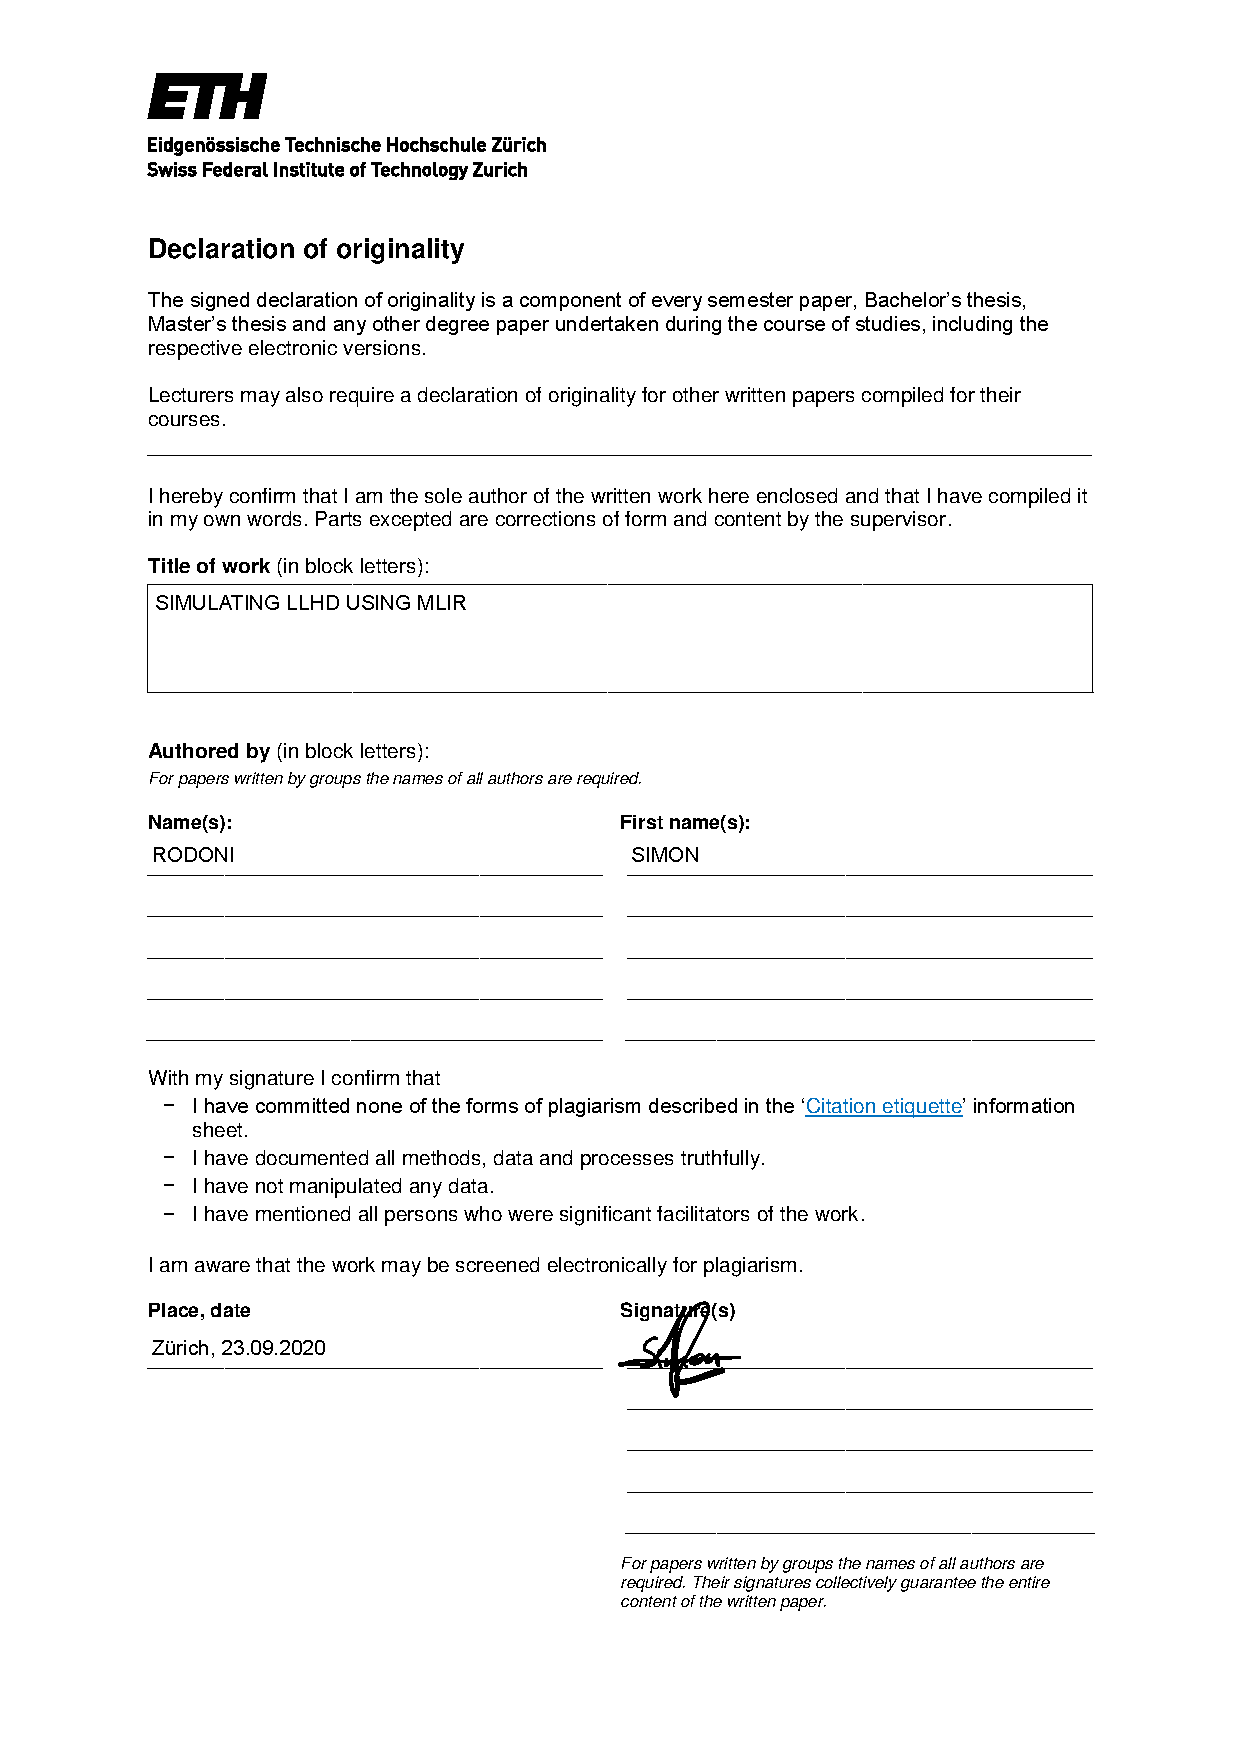
\includepdf[pages={-}]{FrontBackMatter/declaration-originality.pdf}
%----------------------------------------------------------------------------------------

\end{document}
